% ONINU study notes -- generated by _work/pipeline/build_tex.py from markdown.
% Compile with:  latexmk -xelatex optimalno.tex   (lualatex also works)
\documentclass[11pt,a4paper,parskip=half,headsepline,numbers=noenddot]{scrartcl}

% ---------------------------------------------------------------- page layout
\usepackage[a4paper,left=2cm,right=2cm,top=2.4cm,bottom=2.2cm,headheight=15pt,headsep=0.5cm]{geometry}

% ---------------------------------------------------------------- math
\usepackage{amsmath,amssymb}
\usepackage{mathtools}
\usepackage{libertinust1math}  % Libertinus math, matches the text font
\usepackage{bm}

% ---------------------------------------------------------------- fonts and language
\usepackage[no-math]{fontspec}  % no-math: keep the Type1 math fonts set up above
\IfFontExistsTF{LibertinusSerif-Regular.otf}{%
  \setmainfont{LibertinusSerif}[Extension=.otf, UprightFont=*-Regular, BoldFont=*-Bold,
    ItalicFont=*-Italic, BoldItalicFont=*-BoldItalic]
  \setsansfont{LibertinusSans}[Extension=.otf, UprightFont=*-Regular, BoldFont=*-Bold,
    ItalicFont=*-Italic, BoldItalicFont=*-Bold]
}{% fallback: TeX Gyre Pagella / Heros
  \setmainfont{texgyrepagella}[Extension=.otf, UprightFont=*-regular, BoldFont=*-bold,
    ItalicFont=*-italic, BoldItalicFont=*-bolditalic]
  \setsansfont{texgyreheros}[Extension=.otf, UprightFont=*-regular, BoldFont=*-bold,
    ItalicFont=*-italic, BoldItalicFont=*-bolditalic]
}
\setmonofont{lmmono10-regular.otf}[Scale=0.95]
\usepackage[serbian,shorthands=off]{babel}  % Serbian (Latin): Sadržaj, Slika, Tabela
\usepackage{microtype}
\setlength{\emergencystretch}{3em}
% a few Unicode characters that may be typed inside math
\usepackage{newunicodechar}
\newunicodechar{°}{\ifmmode^{\circ}\else\textdegree\fi}
\newunicodechar{≤}{\ensuremath{\leq}}
\newunicodechar{≥}{\ensuremath{\geq}}
\newunicodechar{≠}{\ensuremath{\neq}}
\newunicodechar{≈}{\ensuremath{\approx}}
\newunicodechar{∞}{\ensuremath{\infty}}
\newunicodechar{→}{\ensuremath{\rightarrow}}
\newunicodechar{⇒}{\ensuremath{\Rightarrow}}
\newunicodechar{±}{\ensuremath{\pm}}
\newunicodechar{×}{\ensuremath{\times}}
\newunicodechar{·}{\ensuremath{\cdot}}
\newunicodechar{−}{\ensuremath{-}}
\newunicodechar{ᵀ}{\ensuremath{^{\mathsf{T}}}}

% ---------------------------------------------------------------- colors, boxes
\usepackage{xcolor}
\definecolor{kljucnaC}{HTML}{1F5FA8}
\definecolor{zastoC}{HTML}{2E7D32}
\definecolor{ispitC}{HTML}{C2530A}
\definecolor{izvorC}{HTML}{6B6B6B}
\definecolor{linkC}{HTML}{1A4480}
\usepackage[most]{tcolorbox}
\tcbset{oninu/.style={enhanced, breakable, colback=#1!5, colframe=#1, colbacktitle=#1!14,
    coltitle=#1!75!black, fonttitle=\sffamily\bfseries, boxrule=0.5pt, leftrule=2.5pt,
    arc=1.5pt, left=6pt, right=6pt, top=3pt, bottom=4pt, toptitle=2pt, bottomtitle=2pt,
    before skip=8pt, after skip=10pt, parbox=false}}
% \begin{kljucna}[optional subtitle] ... \end{kljucna}   (same for zasto, ispit)
\newcommand*{\oninutitle}[2]{#1\ifx\relax#2\relax\else: #2\fi}
\newtcolorbox{kljucna}[1][]{oninu=kljucnaC, title={\oninutitle{Ključna ideja}{#1}}}
\newtcolorbox{zasto}[1][]{oninu=zastoC, title={\oninutitle{Zašto?}{#1}}}
\newtcolorbox{ispit}[1][]{oninu=ispitC, title={\oninutitle{Na ispitu}{#1}}}
% Source tag, e.g. \izvor{Khalil 13.2} -> [Khalil 13.2] in small grey type
\DeclareRobustCommand{\izvor}[1]{{\small\color{izvorC}[#1]}}

% ---------------------------------------------------------------- lists, quotes, code
\usepackage{enumitem}
\setlist{itemsep=1pt, topsep=3pt, parsep=1pt}
\providecommand{\tightlist}{}
\renewenvironment{quote}
  {\begin{tcolorbox}[enhanced, breakable, frame hidden, colback=black!4,
    borderline west={2pt}{0pt}{black!30}, sharp corners, left=8pt, before skip=6pt, after skip=8pt]\itshape}
  {\end{tcolorbox}}
\makeatletter
\def\verbatim@font{\small\ttfamily}
\makeatother

% ---------------------------------------------------------------- tables
\usepackage{longtable,booktabs,array,calc}
\newcounter{none}  % pandoc: unnumbered tables
\setlength{\LTpre}{6pt}
\setlength{\LTpost}{6pt}
\renewcommand{\arraystretch}{1.15}

% ---------------------------------------------------------------- figures
\usepackage{graphicx}
\usepackage{float}
\floatplacement{figure}{!htbp}
\usepackage[font=small, labelfont=bf, labelsep=period, format=hang, skip=4pt]{caption}
\makeatletter
\newsavebox\pandoc@box
\newcommand*\pandocbounded[1]{% scale an image to fit the text block
  \sbox\pandoc@box{#1}%
  \Gscale@div\@tempa{\textheight}{\dimexpr\ht\pandoc@box+\dp\pandoc@box\relax}%
  \Gscale@div\@tempb{\linewidth}{\wd\pandoc@box}%
  \ifdim\@tempb\p@<\@tempa\p@\let\@tempa\@tempb\fi
  \ifdim\@tempa\p@<\p@\scalebox{\@tempa}{\usebox\pandoc@box}%
  \else\usebox{\pandoc@box}\fi}
\makeatother

% ---------------------------------------------------------------- shortcuts (optional in the notes)
\providecommand{\R}{\mathbb{R}}
\providecommand{\abs}[1]{\left\lvert #1\right\rvert}
\providecommand{\norm}[1]{\left\lVert #1\right\rVert}
\providecommand{\sgn}{\operatorname{sign}}
\providecommand{\sat}{\operatorname{sat}}
\providecommand{\tr}{\operatorname{tr}}
\providecommand{\rank}{\operatorname{rank}}
\providecommand{\diag}{\operatorname{diag}}
\providecommand{\argmin}{\operatorname*{arg\,min}}
\providecommand{\argmax}{\operatorname*{arg\,max}}

% ---------------------------------------------------------------- headings, header/footer
\setkomafont{disposition}{\sffamily\bfseries\color{kljucnaC!70!black}}
\setkomafont{title}{\sffamily\bfseries\color{kljucnaC!70!black}}
\setcounter{secnumdepth}{0}
\setcounter{tocdepth}{2}
\usepackage{scrlayer-scrpage}
\clearpairofpagestyles
\ihead{\small\sffamily Optimalno upravljanje}
\ohead{\small\sffamily\pagemark}
\pagestyle{scrheadings}

% ---------------------------------------------------------------- links
\usepackage[hyperfootnotes=false]{hyperref}
\hypersetup{colorlinks=true, linkcolor=linkC, urlcolor=linkC, citecolor=linkC,
  pdftitle={Optimalno upravljanje}, pdflang={sr-Latn}, bookmarksnumbered=true, bookmarksopen=true}
\pdfstringdefDisableCommands{\def\izvor#1{}}
\usepackage{bookmark}
\urlstyle{same}

\title{Optimalno upravljanje (Jeličić)}
\subtitle{Beleške za ispit --- prof. Zoran Jeličić (12 pitanja)}
\author{}
\date{\today}

\begin{document}

\maketitle
\thispagestyle{plain.scrheadings}
\tableofcontents
\clearpage

\section{Kako koristiti ove beleške}

\subsection{Format ispita}

Ispit iz optimalnog upravljanja je \textbf{usmeni}, iz \textbf{fiksne liste od 12 pitanja}. Lista je ista kao lista domaćih zadataka, pa je svako pitanje ovde obrađeno kao posebna celina, redom i sa zvaničnim naslovom.

Pitanja su tri vrste:

\begin{itemize}
\item \textbf{Teorijska izvođenja} (pitanja 1--5, 9--11): treba izvesti uslove optimalnosti na tabli, bez preskakanja koraka.
\item \textbf{Računski zadaci} (pitanja 6--8): treba znati postavku, Hamiltonijan, kanonske jednačine, granične uslove i rezultat sa brojevima.
\item \textbf{Simulacije} (pitanje 12): treba znati tri primera LQR sa prezentacije i objasniti grafike.
\end{itemize}

Profesor je na predavanjima više puta rekao da mu je \textbf{numeričko rešenje važnije od analitičkog} i da za zadatke sa ograničenim upravljanjem „ne postoje opšta pravila, samo iskustvo''. Zato uz računske zadatke uvek ide i numerička provera.

\begin{ispit}[{uslovi za ispit}]
\begin{itemize}
\item Profesor: „Ko želi da dođe kod mene na ispit, mora da zna teoriju i \textbf{mora da ima uređene sve domaće}„ \izvor{P14 snimak, 51. min}. Pitanja 6--8 i 12 su upravo ti domaći.
\item MATLAB rešenja domaćih profesor ne daje; na ispitu se brani svoje rešenje.
\item Literatura za HJB: knjiga prof. Vujanovića (izvođenje sa predavanja) ili knjiga Rapajić--Jeličić (tamo je i višedimenzionalni slučaj); „meni je svejedno'' \izvor{P14 snimak, 1. i 51. min}.
\end{itemize}
\end{ispit}

\subsection{Kako je napravljeno svako pitanje}

Svako pitanje (odeljci 1--12) ima isti raspored:

\begin{enumerate}
\def\labelenumi{\arabic{enumi}.}
\item \textbf{Odgovor u 60 sekundi}: 5--8 rečenica koje se mogu reći naglas odmah po izvlačenju pitanja. To je „kostur'' odgovora.
\item \textbf{Ideja}: intuicija u 2--4 rečenice.
\item \textbf{Postavka i izvođenje}: korak po korak, onako kako treba pisati na tabli.
\item \textbf{Primer}: mali zadatak sa brojevima, proveren numerički (skripta \texttt{skripte/\allowbreak{}numerika.py}, rezultati u \texttt{skripte/\allowbreak{}izvestaj\_\allowbreak{}numerike.txt}).
\item \textbf{Ispitna napomena}: šta obavezno reći i gde se najčešće greši.
\end{enumerate}

Zajednički alat (Hamiltonijan, kanonske jednačine i tabela graničnih uslova) je izdvojen u odeljak „Zajednički alat''. Pitanja se na njega pozivaju umesto da ponavljaju ta izvođenja, a svako pitanje zadržava svoj „odgovor u 60 sekundi'' i korake koji su specifični za njega, pa može da se ispriča samostalno.

\subsection{Zavisnosti između pitanja}

\begin{figure}
\centering
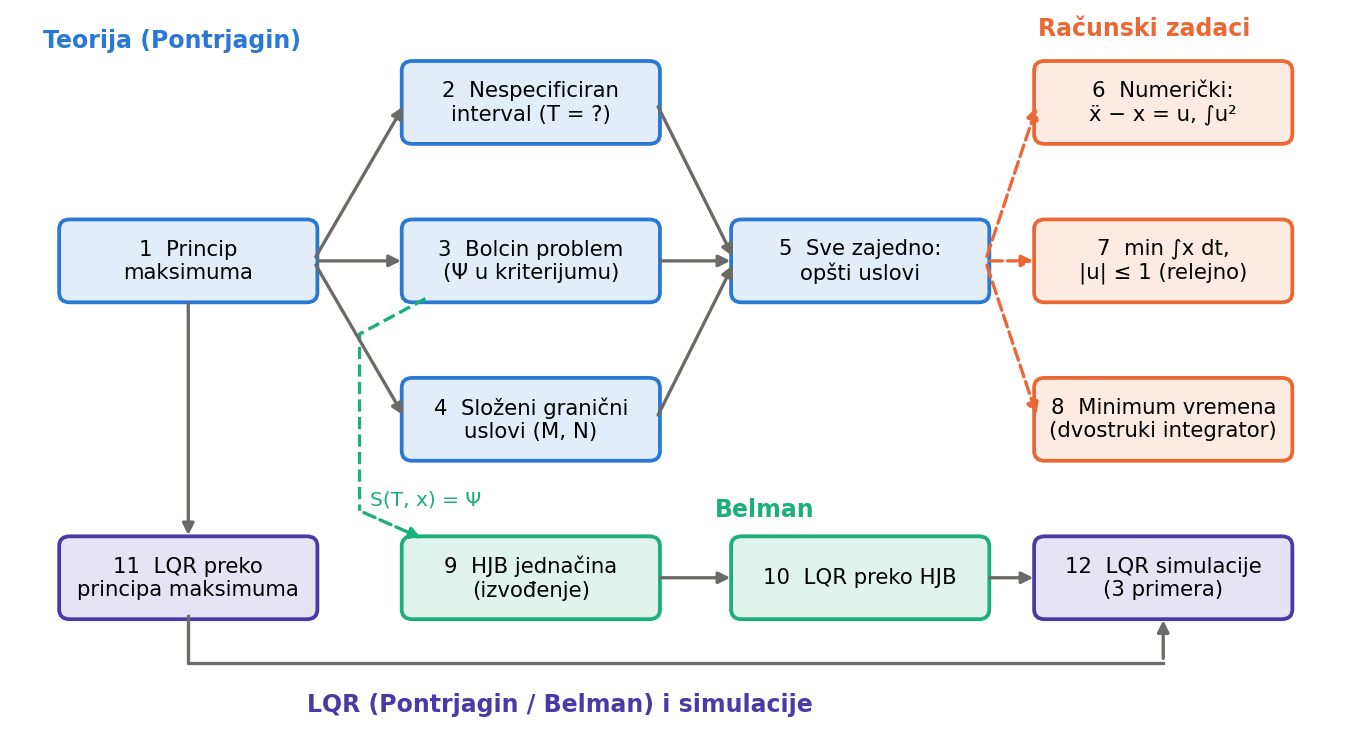
\includegraphics[width=0.9\linewidth,height=\textheight,keepaspectratio,alt={Zavisnosti između 12 ispitnih pitanja. Pitanje 1 je osnova za sve ostalo. Pitanja 2, 3 i 4 dodaju po jedno uopštenje, a pitanje 5 ih spaja. Računski zadaci 6--8 koriste uslove iz 1--5. Belmanova grana (9 → 10) i Pontrjaginova grana (1 → 11) daju istu Rikatijevu jednačinu, koja se koristi u simulacijama (12).}]{figures/f00_zavisnosti.png}
\caption{Zavisnosti između 12 ispitnih pitanja. Pitanje 1 je osnova za sve ostalo. Pitanja 2, 3 i 4 dodaju po jedno uopštenje, a pitanje 5 ih spaja. Računski zadaci 6--8 koriste uslove iz 1--5. Belmanova grana (9 → 10) i Pontrjaginova grana (1 → 11) daju istu Rikatijevu jednačinu, koja se koristi u simulacijama (12).}
\end{figure}

Preporučen redosled učenja:

\begin{enumerate}
\def\labelenumi{\arabic{enumi}.}
\item Odeljak „Zajednički alat'', pa pitanje 1. Bez izvođenja iz pitanja 1 ne može se odgovoriti ni na jedno drugo teorijsko pitanje.
\item Pitanja 2, 3, 4, pa 5. Pitanje 5 je samo zbir prethodna tri: ko zna 2, 3 i 4, zna i 5.
\item Pitanja 7 i 8 (ograničeno upravljanje, relejno rešenje), pa 6 (numerika).
\item Pitanja 9, 10, 11, pa 12.
\end{enumerate}

\subsection{Oznake i konvencija znaka}

\begin{itemize}
\item \(x_i\), \(i = 1, \dots, n\) su promenljive stanja, \(u_k\), \(k = 1, \dots, m\) su upravljanja, a \(p_i\) su pridružene (adjungovane) promenljive, tj. Lagranževi množitelji.
\item Kriterijum optimalnosti (KO) je \(I = \int_0^T F\,dt\) i \textbf{minimizuje se}. Hamiltonijan je \(H = F + \sum p_i f_i\), a optimalno upravljanje \textbf{minimizuje} \(H\).
\item Profesor koristi upravo ovu konvenciju {[}OptControl2022 sl. 4: \(\min_u H\){]}. Ime „princip maksimuma'' je istorijsko: Pontrjagin je pisao \(H = -F + \sum p_i f_i\) i tražio maksimum. Obe konvencije daju isto upravljanje, razlika je samo u znaku \(p\).
\item Izvori se citiraju u zagradama: \izvor{OptControl2022 sl. 7} je slajd profesorove prezentacije.
\end{itemize}

\section{Zajednički alat}

Ovaj odeljak skuplja ono što se koristi u skoro svakom pitanju. Na ispitu ga ne treba pričati posebno: delovi se ubacuju u odgovor tamo gde zatrebaju.

\subsection{Pontrjagin i Belman: dve teorije}

\begin{longtable}[]{@{}
  >{\raggedright\arraybackslash}p{(\linewidth - 4\tabcolsep) * \real{0.1253}}
  >{\raggedright\arraybackslash}p{(\linewidth - 4\tabcolsep) * \real{0.4328}}
  >{\raggedright\arraybackslash}p{(\linewidth - 4\tabcolsep) * \real{0.4419}}@{}}
\caption{Poređenje dve teorije \izvor{OptControl2022 sl. 3--5}}\tabularnewline
\toprule\noalign{}
\begin{minipage}[b]{\linewidth}\raggedright
\end{minipage} & \begin{minipage}[b]{\linewidth}\raggedright
Pontrjagin (1958)
\end{minipage} & \begin{minipage}[b]{\linewidth}\raggedright
Belman (1957)
\end{minipage} \\
\midrule\noalign{}
\endfirsthead
\toprule\noalign{}
\begin{minipage}[b]{\linewidth}\raggedright
\end{minipage} & \begin{minipage}[b]{\linewidth}\raggedright
Pontrjagin (1958)
\end{minipage} & \begin{minipage}[b]{\linewidth}\raggedright
Belman (1957)
\end{minipage} \\
\midrule\noalign{}
\endhead
\bottomrule\noalign{}
\endlastfoot
Alat & varijacioni račun, Lagranževi množitelji \(p_i\) & dinamičko programiranje, funkcija \(S(t, x)\) \\
Jednačine & \(2n\) običnih diferencijalnih jednačina & jedna parcijalna diferencijalna jednačina (HJB) \\
Rešenje & \(u^* = u^*(t)\), \textbf{otvorena sprega} & \(u^* = \Theta(t, x)\), \textbf{zatvorena sprega} \\
Teškoća & dvotačkasti granični problem & parcijalna jednačina po \(t\) i \(x\) \\
\end{longtable}

Profesor ističe da za \textbf{linearni sistem sa kvadratnim kriterijumom} (LQR) obe teorije daju rešenje u zatvorenoj sprezi i istu Rikatijevu jednačinu (pitanja 10 i 11).

\subsection{Problem optimalnog upravljanja}

Sistem je opisan sa \(n\) diferencijalnih jednačina prvog reda:

\[\dot x_i = f_i(t, x_1, \dots, x_n, u_1, \dots, u_m), \qquad i = 1, \dots, n, \qquad x_i(0) = \alpha_i .\]

Traži se upravljanje \(u_k(t)\), \(k = 1, \dots, m\), koje minimizuje kriterijum optimalnosti

\[I = \Psi\big[T, x_i(T)\big] + \int_0^T F(t, x_i, u_k)\,dt .\]

Prema obliku kriterijuma, problem se zove:

\begin{itemize}
\item \textbf{Lagranžov}: samo integral (\(\Psi = 0\)),
\item \textbf{Majerov}: samo \(\Psi\), tj. vrednost na kraju (npr. \(\max z(T)\) u primeru sa robotima na Marsu),
\item \textbf{Bolcin}: i \(\Psi\) i integral (pitanje 3).
\end{itemize}

\subsection{Hamiltonijan i kanonske jednačine}

Hamiltonova funkcija (Hamiltonijan) je

\[H(t, x_i, u_k, p_i) = F(t, x_i, u_k) + \sum_{i=1}^{n} p_i(t)\, f_i(t, x_i, u_k) .\]

Potrebni uslovi optimalnosti (izvedeni u pitanju 1) su:

\[\dot x_i = \frac{\partial H}{\partial p_i} = f_i, \qquad \dot p_i = -\frac{\partial H}{\partial x_i}, \qquad i = 1, \dots, n\]

\[\frac{\partial H}{\partial u_k} = 0, \qquad k = 1, \dots, m \qquad (\text{ako } u \text{ nije ograničeno}).\]

Prve dve grupe se zovu \textbf{kanonske jednačine}: to je \(2n\) diferencijalnih jednačina. Treća grupa je \(m\) algebarskih jednačina iz kojih se izražava \(u_k\) preko \(x\) i \(p\).

Ako je upravljanje \textbf{ograničeno}, \(u_{min} \le u \le u_{max}\), uslov \(\partial H/\partial u = 0\) se zamenjuje opštijim: \(u^*\) je ono dozvoljeno \(u\) koje daje \textbf{najmanji} \(H\). Kada je \(H\) linearan po \(u\), \(H = H_0(x, p) + h(x, p)\,u\), to daje \textbf{relejno} (bang-bang) upravljanje:

\[u^* = \begin{cases} u_{min}, & h > 0 \\ u_{max}, & h < 0 \end{cases}\]

Proizvod \(h\,u\) treba da bude što negativniji, pa \(u\) ide na granicu suprotnog znaka od \(h\) (za maksimizaciju obrnuto). Profesorova slika: tražimo minimum proizvoda dva broja \(a\cdot b\); ako je \(a > 0\), \(b\) mora biti najmanje moguće, a ako je \(a < 0\), najveće moguće. „I to je cela mudrost'' \izvor{P11 snimak, 64. min}. Dokaz ovog pravila je težak i ne traži se; profesor ga radi kroz primere, uz poređenje sa statičkom optimizacijom (kad ne može \(\partial H/\partial u = 0\), rešenje je na granici).

Oznaka: na predavanju o ograničenom upravljanju profesor koeficijent \(h\) uz \(u\) zove \textbf{\(H^*\)} („svi članovi pored upravljanja''). Kod HJB (pitanja 9--10) \(H^*\) znači nešto drugo: Hamiltonijan u koji je uvršteno optimalno \(u\). Na ispitu reći koje značenje se koristi.

\begin{itemize}
\item Broj prekidanja zavisi od toga koliko puta \(h\) menja znak. Ako je \(h\) monotona, prekidanje je najviše jedno. Ako nije (npr. sinusna), prekidanja ima više. Profesor: „Ja ću se truditi da rešavam samo monotone'' \izvor{snimak 25.11, 29. min}.
\item „Tri pomoći'' za izbor strategije: zdrav razum (stabilan ili nestabilan sistem), granični uslov za \(p\) (npr. \(p(T) = 0\) govori šta je na kraju) i vrednost \(p(0)\). „Ne postoji opšte pravilo, svaki problem je za sebe'' \izvor{snimak 25.11, 1. i 14. min}.
\item Ako je \(h \equiv 0\) na nekom intervalu, upravljanje tu nije na granici (singularni luk). Profesor: „teoretski da, praktično ne'', a u zadacima sa ispita se ne javlja \izvor{P11 snimak, 83.--86. min}. Češće je stepeničasto (prošireno relejno) upravljanje, kod minimuma goriva (Dodatak).
\end{itemize}

\subsection{Brojanje uslova}

Dvotačkasti granični problem ima \(2n\) diferencijalnih jednačina, pa traži \(2n\) graničnih uslova. Ako je \(T\) nepoznato, traži se još jedan uslov. Svaki dodatni Lagranžev množitelj (\(\mu_\beta\), \(\lambda_\alpha\)) donosi po jednu nepoznatu, ali i po jednu jednačinu (samo ograničenje \(N_\beta = 0\) ili \(M_\alpha = 0\)). Pravilo za proveru: \textbf{broj nepoznatih mora biti jednak broju jednačina}.

\subsection{Tabela graničnih uslova}

Svi granični uslovi potiču iz istog člana prve varijacije: onog koji je „van integrala'' (pitanja 1--5). Na početku je uvek \(x_i(0) = \alpha_i\), pa je \(\delta x_i(0) = 0\), osim u slučaju složenih uslova na početku.

\begin{longtable}[]{@{}
  >{\raggedright\arraybackslash}p{(\linewidth - 4\tabcolsep) * \real{0.3077}}
  >{\raggedright\arraybackslash}p{(\linewidth - 4\tabcolsep) * \real{0.3077}}
  >{\centering\arraybackslash}p{(\linewidth - 4\tabcolsep) * \real{0.3846}}@{}}
\caption{Granični uslovi (uslovi transverzalnosti); \(\mu^T\partial N/\partial x\) je skraćeno za \(\sum_\beta\mu_\beta\,\partial N_\beta/\partial x_i\) \izvor{OptControl2022 sl. 9}}\tabularnewline
\toprule\noalign{}
\begin{minipage}[b]{\linewidth}\raggedright
Situacija na kraju
\end{minipage} & \begin{minipage}[b]{\linewidth}\raggedright
Uslov
\end{minipage} & \begin{minipage}[b]{\linewidth}\centering
Pitanje
\end{minipage} \\
\midrule\noalign{}
\endfirsthead
\toprule\noalign{}
\begin{minipage}[b]{\linewidth}\raggedright
Situacija na kraju
\end{minipage} & \begin{minipage}[b]{\linewidth}\raggedright
Uslov
\end{minipage} & \begin{minipage}[b]{\linewidth}\centering
Pitanje
\end{minipage} \\
\midrule\noalign{}
\endhead
\bottomrule\noalign{}
\endlastfoot
\(x_i(T) = \beta_i\) zadato & \(x_i(T) = \beta_i\), a \(p_i(T)\) je nepoznato & 1, 6, 8 \\
\(x_i(T)\) slobodno & \(p_i(T) = 0\) (prirodni granični uslov) & 1, 7 \\
Bolca, \(x_i(T)\) slobodno & \(p_i(T) = \partial\Psi/\partial x_i(T)\) & 3 \\
kraj na mnogostrukosti \(N_\beta = 0\), \(\beta = 1, \dots, r\) & \(N = 0\) i \(p(T) = \partial\Psi/\partial x + \mu^T\partial N/\partial x\) (u \(T\)) & 4, 5 \\
početak na mnogostrukosti \(M_\alpha = 0\) & \(M = 0\) i \(p(0) = \partial\Psi/\partial x + \lambda^T\partial M/\partial x\) (u 0) & 4 \\
\(T\) nepoznato (opšti slučaj) & \(H(T) + \partial\Psi/\partial T + \mu^T\partial N/\partial T = 0\) & 5 \\
\(T\) nepoznato, \(\Psi\) i \(N\) ne zavise od \(T\) & \(H(T) = 0\) & 2, 8 \\
\(T\) nepoznato i sistem autonoman & \(H(t) \equiv 0\) na celoj putanji & 2, 8 \\
\end{longtable}

\begin{kljucna}
Jedno pravilo pokriva celu tabelu: \textbf{za svaku veličinu koja je slobodna} (neko \(x_i(T)\), ili \(T\)), njen koeficijent u prvoj varijaciji mora biti nula. Zadate veličine daju sam uslov (\(x_i(T) = \beta_i\)), a slobodne daju uslov za \(p\) ili za \(H\).
\end{kljucna}

\subsection{\texorpdfstring{Osobina \(H = \text{const}\)}{Osobina H = \textbackslash text\{const\}}}

Duž optimalne putanje je

\[\frac{dH}{dt} = \sum_i \frac{\partial H}{\partial x_i}\dot x_i + \sum_i \frac{\partial H}{\partial p_i}\dot p_i + \sum_k \frac{\partial H}{\partial u_k}\dot u_k + \frac{\partial H}{\partial t} .\]

Kad se ubace kanonske jednačine, prve dve sume su \(\sum_i \big(-\dot p_i \dot x_i + \dot x_i \dot p_i\big) = 0\). Treća suma je nula jer je \(\partial H/\partial u_k = 0\) (kod relejnog upravljanja je \(\dot u = 0\) svuda osim u trenucima prekidanja, a u trenutku prekidanja je \(h = 0\), pa skok \(u\) ne menja \(H = H_0 + h\,u\)). Ostaje

\[\frac{dH}{dt} = \frac{\partial H}{\partial t} .\]

Ako \(F\) i \(f_i\) ne zavise eksplicitno od \(t\) (autonoman sistem), onda je \textbf{\(H = \text{const}\)} duž optimalne putanje \izvor{OptControl2022 sl. 10}. Ovo se koristi kao \textbf{provera rešenja}: izračuna se \(H(t)\) i proveri da li je konstantan.

\section{1. Optimalno upravljanje, princip maksimuma}

\begin{kljucna}[{Odgovor u 60 sekundi}]
\begin{enumerate}
\def\labelenumi{\arabic{enumi}.}
\item Sistem \(\dot x_i = f_i(t, x, u)\), \(x_i(0) = \alpha_i\), traži se \(u(t)\) koje minimizuje \(I = \int_0^T F\,dt\); \(T\) je poznato.
\item Dinamika se u kriterijum uvodi Lagranževim množiteljima \(p_i(t)\): \(\bar I = \int_0^T \big[F - \sum p_i(\dot x_i - f_i)\big]dt\).
\item Uvodi se Hamiltonijan \(H = F + \sum p_i f_i\), pa je \(\bar I = \int_0^T \big[H - \sum p_i \dot x_i\big]dt\).
\item Potreban uslov je \(\delta \bar I = 0\). Član \(p_i\,\delta\dot x_i\) se parcijalno integrali.
\item Svaki koeficijent uz \(\delta x_i\), \(\delta p_i\), \(\delta u_k\) mora biti nula: \(\dot x_i = \partial H/\partial p_i\), \(\dot p_i = -\partial H/\partial x_i\), \(\partial H/\partial u_k = 0\).
\item Član van integrala daje granični uslov: \(x_i(0) = \alpha_i\) i, ako je kraj slobodan, \(p_i(T) = 0\).
\item Dobija se dvotačkasti granični problem; rešenje je \(u^*(t)\), u otvorenoj sprezi. Za autonoman sistem \(H = \text{const}\).
\end{enumerate}
\end{kljucna}

\subsection{Ideja}

Tražimo funkciju \(u(t)\), a ne broj, pa je ovo problem varijacionog računa. Sistem je ograničenje koje mora da važi u svakom trenutku, pa se u kriterijum uvodi sa Lagranževim množiteljem koji je \textbf{funkcija vremena}, \(p_i(t)\). Tako problem sa ograničenjem postaje problem bez ograničenja, a uslov optimalnosti je da je prva varijacija proširenog kriterijuma jednaka nuli, isto kao što je kod funkcije uslov da je prvi izvod nula.

\subsection{Postavka}

\[\dot x_i = f_i(t, x_i, u_k), \qquad i = 1, \dots, n, \qquad k = 1, \dots, m, \qquad 0 \le t \le T\]

\[x_i(0) = \alpha_i \quad (\text{poznato}), \qquad T \text{ poznato}\]

\[I = \int_0^T F(t, x_i, u_k)\,dt \;\to\; \min\]

Upravljanje za sada nije ograničeno. \izvor{OptControl2022 sl. 7}

\subsection{Izvođenje}

\textbf{Korak 1: prošireni kriterijum.} Ograničenje \(\dot x_i - f_i = 0\) se množi sa \(p_i(t)\) i oduzima od podintegralne funkcije. Pošto je zagrada nula na svakoj dopustivoj putanji, vrednost kriterijuma se ne menja:

\[\bar I = \int_0^T \Big\{ F(t, x_i, u_k) - \sum_{i=1}^n p_i(t)\big[\dot x_i - f_i(t, x_i, u_k)\big] \Big\} dt .\]

\begin{zasto}
Zašto \(p_i(t)\), a ne konstanta? Ograničenje \(\dot x_i = f_i\) važi u svakom trenutku, tj. to je beskonačno mnogo ograničenja (po jedno za svako \(t\)), pa svako dobija svoj množitelj. Znak ispred zagrade je stvar izbora: sa „\(-\)„ se dobija \(H = F + \sum p_i f_i\); sa „\(+\)„ bi se samo promenio znak \(p\).
\end{zasto}

\textbf{Korak 2: Hamiltonijan.} Grupišu se članovi koji ne sadrže \(\dot x_i\):

\[H(t, x_i, u_k, p_i) \overset{def}{=} F(t, x_i, u_k) + \sum_{i=1}^n p_i(t)\, f_i(t, x_i, u_k)\]

\[\bar I = \int_0^T \Big[ H(t, x_i, u_k, p_i) - \sum_{i=1}^n p_i \dot x_i \Big] dt .\]

\textbf{Korak 3: prva varijacija.} \(T\) je poznato, pa se varira samo podintegralna funkcija. Variraju se \(x_i\), \(p_i\) i \(u_k\) (i \(\dot x_i\), kao posledica \(\delta x_i\)):

\[\delta \bar I = \int_0^T \Big\{ \sum_{i=1}^n \Big[ \frac{\partial H}{\partial x_i}\delta x_i + \frac{\partial H}{\partial p_i}\delta p_i - \dot x_i\,\delta p_i - p_i\,\delta \dot x_i \Big] + \sum_{k=1}^m \frac{\partial H}{\partial u_k}\delta u_k \Big\} dt .\]

\textbf{Korak 4: parcijalna integracija.} Član \(p_i\,\delta\dot x_i\) sadrži varijaciju izvoda, pa se prebacuje na \(\delta x_i\). Iz pravila za izvod proizvoda:

\[\frac{d}{dt}\big(p_i\,\delta x_i\big) = \dot p_i\,\delta x_i + p_i\,\delta\dot x_i \quad\Rightarrow\quad -p_i\,\delta\dot x_i = \dot p_i\,\delta x_i - \frac{d}{dt}\big(p_i\,\delta x_i\big) .\]

Integral od \(\frac{d}{dt}(p_i\delta x_i)\) je \(p_i\delta x_i\big|_0^T\), pa je

\[\delta \bar I = -\sum_{i=1}^n p_i\,\delta x_i\Big|_0^T + \int_0^T \Big\{ \sum_{i=1}^n \Big[ \Big(\frac{\partial H}{\partial x_i} + \dot p_i\Big)\delta x_i + \Big(\frac{\partial H}{\partial p_i} - \dot x_i\Big)\delta p_i \Big] + \sum_{k=1}^m \frac{\partial H}{\partial u_k}\delta u_k \Big\} dt = 0 .\]

\textbf{Korak 5: uslovi pod integralom.} Varijacije \(\delta x_i\), \(\delta p_i\), \(\delta u_k\) su proizvoljne funkcije. Integral je nula za svaki njihov izbor samo ako je svaki koeficijent nula:

\[\dot x_i = \frac{\partial H}{\partial p_i} = f_i(t, x_i, u_k), \qquad \dot p_i = -\frac{\partial H}{\partial x_i} = -\frac{\partial F}{\partial x_i} - \sum_{j=1}^n p_j\frac{\partial f_j}{\partial x_i}, \qquad \frac{\partial H}{\partial u_k} = 0 .\]

\begin{zasto}
Strogo gledano, \(\delta x_i\) nije nezavisno od \(\delta u_k\): promena upravljanja menja putanju. Zato se redosled argumenta čita ovako: \(p_i(t)\) još nije određeno, pa ga \textbf{biramo} tako da koeficijent uz \(\delta x_i\) bude nula (\(\dot p_i = -\partial H/\partial x_i\)). Tada ostaje samo član sa \(\delta u_k\), a \(\delta u_k\) jeste proizvoljno, pa mora biti \(\partial H/\partial u_k = 0\).
\end{zasto}

Prva jednačina je sam sistem: uvođenje \(p_i\) ga nije promenilo. Druga je jednačina za \(p_i\) (profesor je zove „generalisani impuls''). Treća daje \(u_k\) kao funkciju \(x\) i \(p\).

\textbf{Korak 6: uslov van integrala.} Ostaje

\[-\sum_{i=1}^n p_i\,\delta x_i\Big|_0^T = -\sum_{i=1}^n p_i(T)\,\delta x_i(T) + \sum_{i=1}^n p_i(0)\,\delta x_i(0) = 0 .\]

\begin{itemize}
\item Na početku je \(x_i(0) = \alpha_i\) zadato, pa je \(\delta x_i(0) = 0\) i drugi član nestaje.
\item Ako je \(x_i(T)\) \textbf{slobodno}, \(\delta x_i(T)\) je proizvoljno, pa mora biti \(p_i(T) = 0\). To je \textbf{prirodni granični uslov}: nije zadat, nego ga je dala sama optimizacija.
\item Ako je \(x_i(T) = \beta_i\) \textbf{zadato}, onda je \(\delta x_i(T) = 0\), član nestaje, a \(p_i(T)\) ostaje nepoznato. Umesto uslova \(p_i(T) = 0\) koristi se \(x_i(T) = \beta_i\).
\end{itemize}

\begin{kljucna}
\textbf{Dvotačkasti granični problem} (Two Point Boundary Value Problem) \izvor{OptControl2022 sl. 4, 9}:

\[\dot x_i = \frac{\partial H}{\partial p_i}, \quad \dot p_i = -\frac{\partial H}{\partial x_i}, \quad \frac{\partial H}{\partial u_k} = 0, \quad x_i(0) = \alpha_i, \quad p_i(T) = 0 .\]

Rešenje je \(u_k^* = u_k^*(t)\): upravljanje u \textbf{otvorenoj sprezi}.
\end{kljucna}

\textbf{Zašto je problem težak.} Za \(x\) su uslovi zadati na početku, a za \(p\) na kraju. Zato se sistem od \(2n\) jednačina ne može jednostavno integraliti ni unapred ni unazad. Numerički se rešava iterativno (FBSM, pitanje 6).

\textbf{Korak 7: dovoljan uslov.} \(\partial H/\partial u = 0\) daje stacionarnu tačku. Da bi to bio minimum, mora biti \(\partial^2 H/\partial u_k^2 \ge 0\) (za maksimum \(\le 0\)) \izvor{OptControl2022 sl. 9}. Kod više upravljanja to je uslov da je matrica \(\partial^2 H/\partial u^2\) pozitivno semidefinitna. Pažnja: ovaj uslov (Ležandr--Klebš) garantuje samo da \(u^*\) minimizuje \(H\) u svakom trenutku, pri datim \(x\) i \(p\). On ne garantuje da je cela putanja globalni minimum \(I\). Za to je potrebna konveksnost: ako je sistem linearan, a \(F\) i \(\Psi\) konveksni po \((x, u)\) (npr. LQR), potrebni uslovi su i dovoljni.

\textbf{Korak 8: \(H = \text{const}\).} Za autonoman sistem \(dH/dt = \partial H/\partial t = 0\) (izvedeno u odeljku „Zajednički alat''). Konstantno \(H\) je dobra provera rešenja.

\textbf{Korak 9: ograničeno upravljanje.} Ako je \(u_{min} \le u \le u_{max}\), optimum može biti na granici, gde je \(\partial H/\partial u \ne 0\). Tada važi opštiji oblik principa: \(u^*\) \textbf{minimizuje \(H\)} po svim dozvoljenim \(u\):

\[H(t, x^*, u^*, p) \le H(t, x^*, u, p) \qquad \text{za svako dozvoljeno } u .\]

Ako je \(H\) linearan po \(u\), rešenje je relejno (pitanja 7 i 8). Ovo je pravi „princip maksimuma'' (minimuma), a \(\partial H/\partial u = 0\) je samo njegov specijalan slučaj za unutrašnji optimum \izvor{OptControl2022 sl. 4}.

\subsection{Primer A: slobodan kraj}

\[\dot x = u, \qquad x(0) = 1, \qquad I = \frac12\int_0^1 \big(x^2 + u^2\big)dt, \qquad x(1) \text{ slobodno.}\]

\textbf{Hamiltonijan i uslovi.}

\[H = \tfrac12 x^2 + \tfrac12 u^2 + p\,u\]

\[\frac{\partial H}{\partial u} = u + p = 0 \;\Rightarrow\; u^* = -p, \qquad \dot p = -\frac{\partial H}{\partial x} = -x, \qquad \dot x = u = -p .\]

Granični uslovi: \(x(0) = 1\) i, pošto je \(x(1)\) slobodno, \(p(1) = 0\). Dovoljan uslov: \(\partial^2 H/\partial u^2 = 1 > 0\), pa je to minimum.

\textbf{Rešavanje.} Diferenciranjem \(\dot x = -p\) dobija se \(\ddot x = -\dot p = x\). Rešenje je \(x(t) = A\cosh(1 - t) + B\sinh(1 - t)\). Uslov \(p(1) = 0\) znači \(\dot x(1) = 0\):

\[\dot x(t) = -A\sinh(1-t) - B\cosh(1-t), \qquad \dot x(1) = -B = 0 .\]

Iz \(x(0) = A\cosh 1 = 1\) sledi \(A = 1/\cosh 1\):

\[x^*(t) = \frac{\cosh(1-t)}{\cosh 1}, \qquad u^*(t) = \dot x = -\frac{\sinh(1-t)}{\cosh 1}, \qquad p(t) = -u^* = \frac{\sinh(1-t)}{\cosh 1} .\]

\textbf{Provera \(H = \text{const}\).} Sa \(u = -p\) je \(H = \frac12 x^2 - \frac12 u^2 = \frac{\cosh^2(1-t) - \sinh^2(1-t)}{2\cosh^2 1} = \frac{1}{2\cosh^2 1} = 0{,}21\), konstantno. Vrednost kriterijuma je \(I = \frac12\tanh 1 = 0{,}3808\) (numerički proverene obe vrednosti).

\begin{figure}
\centering
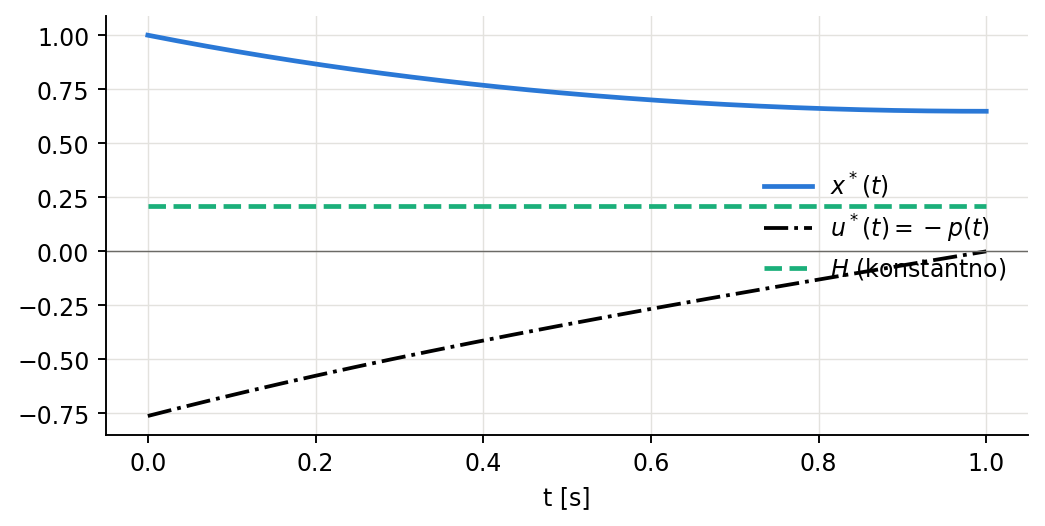
\includegraphics[width=0.75\linewidth,height=\textheight,keepaspectratio,alt={Primer A. Upravljanje je najjače na početku, dok je x veliko, i pada na nulu na kraju, jer je p(1) = 0. Hamiltonijan je konstantan, što potvrđuje da je rešenje ispravno.}]{figures/q1_primer_slobodan_kraj.png}
\caption{Primer A. Upravljanje je najjače na početku, dok je x veliko, i pada na nulu na kraju, jer je p(1) = 0. Hamiltonijan je konstantan, što potvrđuje da je rešenje ispravno.}
\end{figure}

\subsection{Primer B: zadat kraj (primer sa slajda)}

Profesorov primer \izvor{OptControl2022 sl. 11}:

\[\dot x_1 = x_2, \qquad \dot x_2 = -x_2 + u, \qquad I = \frac12\int_0^2 u^2\,dt, \qquad x(0) = (0, 0), \quad x(2) = (5, 2) .\]

(Na slajdu u drugoj jednačini piše \(\dot x_1\), što je greška u kucanju: mora biti \(\dot x_2\).)

\textbf{Hamiltonijan i uslovi.}

\[H = \tfrac12 u^2 + p_1 x_2 + p_2(-x_2 + u), \qquad \frac{\partial H}{\partial u} = u + p_2 = 0 \;\Rightarrow\; u^* = -p_2\]

\[\dot p_1 = -\frac{\partial H}{\partial x_1} = 0 \;\Rightarrow\; p_1 = c_1, \qquad \dot p_2 = -\frac{\partial H}{\partial x_2} = -p_1 + p_2 \;\Rightarrow\; p_2 = c_1 + c_2 e^{t} .\]

Oba kraja su zadata, pa nema uslova za \(p\): konstante \(c_1, c_2\) se određuju iz \(x(2) = (5, 2)\).

\textbf{Stanja.} \(u = -c_1 - c_2e^t\). Jednačina \(\dot x_2 + x_2 = -c_1 - c_2 e^t\) sa \(x_2(0) = 0\) daje (partikularno rešenje \(-c_1 - \frac{c_2}{2}e^t\), homogeno \(Ce^{-t}\)):

\[x_2(t) = -c_1\big(1 - e^{-t}\big) - c_2\sinh t, \qquad x_1(t) = \int_0^t x_2\,d\tau = -c_1\big(t - 1 + e^{-t}\big) - c_2\big(\cosh t - 1\big) .\]

\textbf{Konstante.} Iz \(x_2(2) = 2\) i \(x_1(2) = 5\):

\[-0{,}8647\,c_1 - 3{,}6269\,c_2 = 2, \qquad -1{,}1353\,c_1 - 2{,}7622\,c_2 = 5 \;\Rightarrow\; c_1 = -7{,}2918, \quad c_2 = 1{,}1870 .\]

\[u^*(t) = 7{,}2918 - 1{,}1870\,e^{t}, \qquad u(0) = 6{,}10, \quad u(2) = -1{,}48, \qquad I = 16{,}75 .\]

Provera: \(H = -18{,}63\) na celom intervalu (konstantno, ali ne nula, jer je \(T\) zadato).

\begin{figure}
\centering
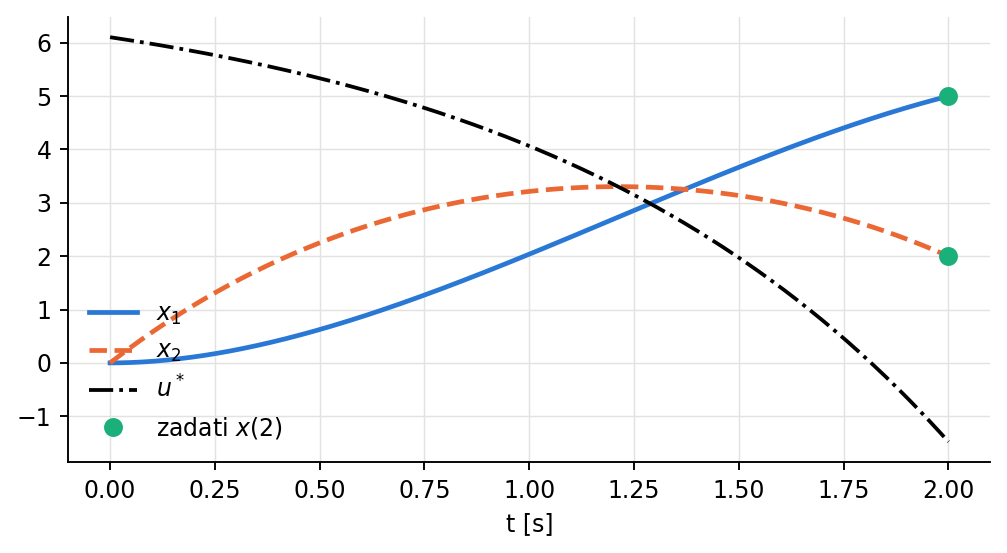
\includegraphics[width=0.75\linewidth,height=\textheight,keepaspectratio,alt={Primer sa slajda 11, ponovo izračunat. Upravljanje je glatko (eksponencijalno), jer je H kvadratan po u. Pri kraju je u \textless{} 0: sistem mora da uspori da bi stigao u x₂(2) = 2. Krive se poklapaju sa slajdom.}]{figures/q1_primer_slajd.png}
\caption{Primer sa slajda 11, ponovo izračunat. Upravljanje je glatko (eksponencijalno), jer je H kvadratan po u. Pri kraju je u \textless{} 0: sistem mora da uspori da bi stigao u x₂(2) = 2. Krive se poklapaju sa slajdom.}
\end{figure}

\begin{ispit}[{Pitanje 1}]
\begin{itemize}
\item Obavezno: prošireni KO, definicija \(H\), prva varijacija, \textbf{parcijalna integracija} člana \(p_i\delta\dot x_i\), tri grupe uslova, granični uslov \(p_i(T) = 0\) i objašnjenje odakle dolazi.
\item Reći da je rešenje u \textbf{otvorenoj} sprezi i da je problem \textbf{dvotačkasti}.
\item Zamka: \(\partial H/\partial u = 0\) važi samo za neograničeno upravljanje. Opšti princip je \(\min_u H\).
\item Zamka: kad je \(x_i(T)\) zadato, \(p_i(T)\) \textbf{nije} nula.
\end{itemize}
\end{ispit}

\subsection{Moguća potpitanja}

\begin{itemize}
\item \textbf{Zašto je \(p(T) = 0\)?} Član van integrala je \(-p_i(T)\delta x_i(T)\). Ako je \(x_i(T)\) slobodno, \(\delta x_i(T)\) je proizvoljno, pa član nestaje za svaki izbor samo ako je \(p_i(T) = 0\).
\item \textbf{Šta ako je \(x(T)\) zadato?} Tada je \(\delta x_i(T) = 0\), nema uslova za \(p_i(T)\); umesto njega važi \(x_i(T) = \beta_i\) (primer B). Broj uslova ostaje \(2n\).
\item \textbf{Šta ako je \(T\) slobodno?} Dobija se još jedan uslov, \(H(T) = 0\) (pitanje 2).
\item \textbf{Šta fizički predstavlja \(p\)?} Osetljivost optimalne vrednosti kriterijuma na stanje: \(p_i(t) = \partial S/\partial x_i\) (veza sa Belmanom, pitanje 9). Zato je \(p(T) = 0\) kad kraj ništa ne košta.
\item \textbf{Kada je Pontrjaginov uslov i dovoljan?} Kad je problem konveksan: linearan sistem, \(F\) konveksno po \((x, u)\) (npr. LQR). Inače su uslovi samo potrebni, a \(\partial^2 H/\partial u^2 > 0\) potvrđuje samo minimum \(H\) po \(u\).
\item \textbf{Zašto je rešenje u otvorenoj sprezi?} Iz TPBVP se dobija funkcija vremena \(u^*(t)\) za jedno konkretno \(x(0)\); za drugo početno stanje sve se računa ponovo.
\end{itemize}

\section{2. Optimalno upravljanje, slučaj nespecificiranog vremenskog intervala}

\begin{kljucna}[{Odgovor u 60 sekundi}]
\begin{enumerate}
\def\labelenumi{\arabic{enumi}.}
\item Isto kao pitanje 1, ali je krajnje vreme \(T\) nepoznato: to je jedna nepoznata više, pa treba jedan uslov više.
\item Zato se koristi \textbf{asinhrona varijacija}: varira se i putanja i trenutak završetka, \(\Delta x = \delta x + \dot x\,\Delta t\).
\item Varijacija integrala sa promenljivom gornjom granicom dobija član \([H - \sum p_i\dot x_i]_{t=T}\Delta T\).
\item Kanonske jednačine i \(\partial H/\partial u = 0\) ostaju iste kao u pitanju 1.
\item Novi član van integrala je \(-\sum p_i(T)\Delta x_i(T) + H(T)\Delta T\).
\item Pošto je \(\Delta T\) proizvoljno, dobija se novi uslov \(H(T) = 0\); za autonoman sistem je onda \(H \equiv 0\) duž cele putanje.
\item Tipičan primer je problem minimuma vremena (\(F = 1\)).
\end{enumerate}
\end{kljucna}

\subsection{Ideja}

Kad \(T\) nije zadato, optimizacija bira i \textbf{koliko dugo} traje proces. Varirana putanja zato može da se završi i ranije i kasnije od optimalne. Kriterijum ne sme da se smanji ni za malo produženje ni za malo skraćenje intervala. Iz toga se dobija dodatni uslov, i to baš za Hamiltonijan: \(H(T) = 0\).

\subsection{Postavka}

\[\dot x_i = f_i(t, x_i, u_k), \qquad x_i(0) = \alpha_i, \qquad x_i(T) = \beta_i, \qquad T = \;?\]

\[I = \int_0^T F(t, x_i, u_k)\,dt \;\to\; \min\]

Nepoznate su: \(2n\) konstanti integracije kanonskih jednačina i \(T\), ukupno \(2n + 1\). Uslova iz pitanja 1 ima \(2n\) (\(n\) na početku, \(n\) na kraju). Fali jedan.

\subsection{Izvođenje}

\textbf{Korak 1: asinhrona varijacija stanja.} Optimalna putanja \(x^*(t)\) završava u \(T\), a varirana \(x^* + \delta x\) u \(T + \Delta T\). Ukupna promena stanja na kraju je

\[\Delta x_i(T) = \big[x_i^* + \delta x_i\big](T + \Delta T) - x_i^*(T) \approx \delta x_i(T) + \dot x_i(T)\,\Delta T .\]

Prvi član je promena putanje u istom trenutku (sinhrona varijacija), a drugi je promena zbog pomeranja kraja.

\begin{figure}
\centering
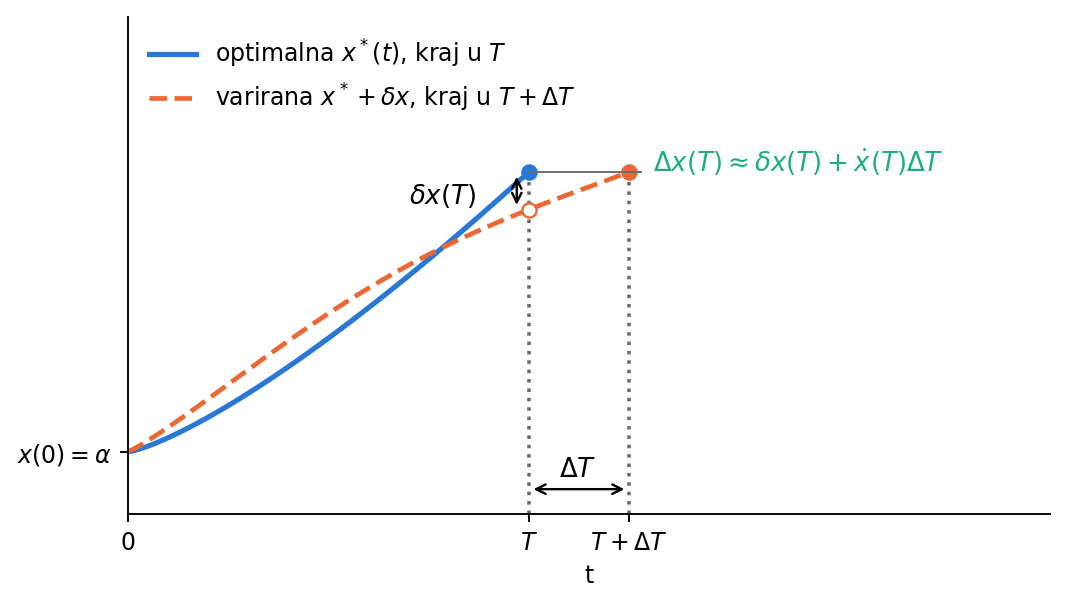
\includegraphics[width=0.7\linewidth,height=\textheight,keepaspectratio,alt={Asinhrona varijacija. Varirana putanja (isprekidano) završava u T + ΔT. Ukupna promena kraja Δx(T) ima dva dela: δx(T) (razlika putanja u istom trenutku T) i ẋ(T)ΔT (pomeraj duž putanje zbog dužeg intervala).}]{figures/q2_asinhrona_varijacija.png}
\caption{Asinhrona varijacija. Varirana putanja (isprekidano) završava u T + ΔT. Ukupna promena kraja Δx(T) ima dva dela: δx(T) (razlika putanja u istom trenutku T) i ẋ(T)ΔT (pomeraj duž putanje zbog dužeg intervala).}
\end{figure}

\textbf{Korak 2: varijacija integrala sa promenljivom granicom.} Za bilo koju podintegralnu funkciju \(G\):

\[\Delta\int_0^T G\,dt = \int_0^{T + \Delta T}(G + \delta G)\,dt - \int_0^T G\,dt = \int_0^T \delta G\,dt + \int_T^{T+\Delta T} G\,dt \approx \delta\int_0^T G\,dt + G(T)\,\Delta T .\]

\textbf{Korak 3: primena na prošireni kriterijum.} Prošireni kriterijum je isti kao u pitanju 1, \(\bar I = \int_0^T[H - \sum p_i\dot x_i]dt\). Sa \(G = H - \sum p_i \dot x_i\), sinhroni deo \(\delta\int G\,dt\) je već izračunat u pitanju 1 (koraci 3 i 4: prva varijacija i parcijalna integracija), pa je

\[\Delta\bar I = -\sum_{i=1}^n p_i\,\delta x_i\Big|_0^T + \int_0^T\{\dots\}\,dt + \Big[H - \sum_{i=1}^n p_i\dot x_i\Big]_{t=T}\Delta T ,\]

gde je \(\{\dots\}\) podintegralni izraz iz pitanja 1 (koeficijenti uz \(\delta x_i\), \(\delta p_i\), \(\delta u_k\)). Poslednji član je \textbf{član asinhrone varijacije}.

\textbf{Korak 4: spajanje članova na kraju.} Na početku je \(\delta x_i(0) = 0\). Na kraju se skupe dva člana sa \(p_i(T)\):

\[-\sum_i p_i(T)\,\delta x_i(T) - \sum_i p_i(T)\,\dot x_i(T)\,\Delta T = -\sum_i p_i(T)\big[\delta x_i(T) + \dot x_i(T)\Delta T\big] = -\sum_i p_i(T)\,\Delta x_i(T) .\]

Ostaje

\[\Delta\bar I = -\sum_{i=1}^n p_i(T)\,\Delta x_i(T) + H(T)\,\Delta T + \int_0^T\{\dots\}\,dt = 0 .\]

\textbf{Korak 5: uslovi.} Pod integralom je sve isto kao u pitanju 1: kanonske jednačine i \(\partial H/\partial u_k = 0\) (odeljak „Zajednički alat''). Van integrala:

\begin{itemize}
\item \(x_i(T) = \beta_i\) je zadato, pa je ukupna promena \(\Delta x_i(T) = 0\) (varirana putanja takođe mora da stigne u \(\beta_i\), samo u drugom trenutku).
\item \(\Delta T\) je proizvoljno (to je baš nepoznata), pa njegov koeficijent mora biti nula:
\end{itemize}

\begin{kljucna}
\[H(T) = 0 .\]

Ako je i \(x_i(T)\) slobodno, dodaje se još \(p_i(T) = 0\). Ako sistem i \(F\) ne zavise eksplicitno od \(t\), onda je \(H = \text{const}\) (odeljak „Zajednički alat''), pa je \textbf{\(H(t) \equiv 0\) duž cele optimalne putanje}.
\end{kljucna}

\textbf{Korak 6: brojanje.} Sada ima \(2n + 1\) uslova (\(x_i(0) = \alpha_i\), \(x_i(T) = \beta_i\), \(H(T) = 0\)) za \(2n + 1\) nepoznatih. Problem je dobro postavljen.

\textbf{Zašto \(H(T) = 0\) ima smisla.} Kad bi bilo \(H(T) > 0\), skraćenje intervala za \(\Delta T < 0\) bi smanjilo kriterijum, a kad bi bilo \(H(T) < 0\), isplatilo bi se produženje. Na optimalnom \(T\) nijedno od toga ne sme da pomogne.

\subsection{Primer: kompromis vreme--energija}

\[\dot x = u, \qquad x(0) = 0, \qquad x(T) = 1, \qquad I = \int_0^T \big(1 + u^2\big)dt, \qquad T = \;?\]

Jedinica u \(F\) „kažnjava'' trajanje, a \(u^2\) kažnjava utrošenu energiju. Brzo stizanje troši mnogo energije, a sporo traje dugo.

\textbf{Uslovi.}

\[H = 1 + u^2 + p\,u, \qquad \frac{\partial H}{\partial u} = 2u + p = 0 \;\Rightarrow\; u = -\frac p2, \qquad \dot p = -\frac{\partial H}{\partial x} = 0 \;\Rightarrow\; p = \text{const} .\]

Znači \(u\) je konstantno, \(x(t) = u\,t\), a iz \(x(T) = 1\) sledi \(u = 1/T\).

\textbf{Uslov za \(T\).} Sa \(p = -2u\):

\[H = 1 + u^2 - 2u^2 = 1 - u^2 = 0 \;\Rightarrow\; u = 1 \quad (u > 0, \text{ jer } x \text{ raste od 0 do 1}) \;\Rightarrow\; T = 1, \quad I = 2 .\]

\textbf{Provera direktno.} Za bilo koje \(T\) je najbolje konstantno \(u = 1/T\), pa je \(I(T) = \int_0^T\big(1 + 1/T^2\big)dt = T + 1/T\). Izvod \(1 - 1/T^2 = 0\) daje \(T = 1\) i \(I = 2\), isto kao iz uslova \(H(T) = 0\).

\begin{figure}
\centering
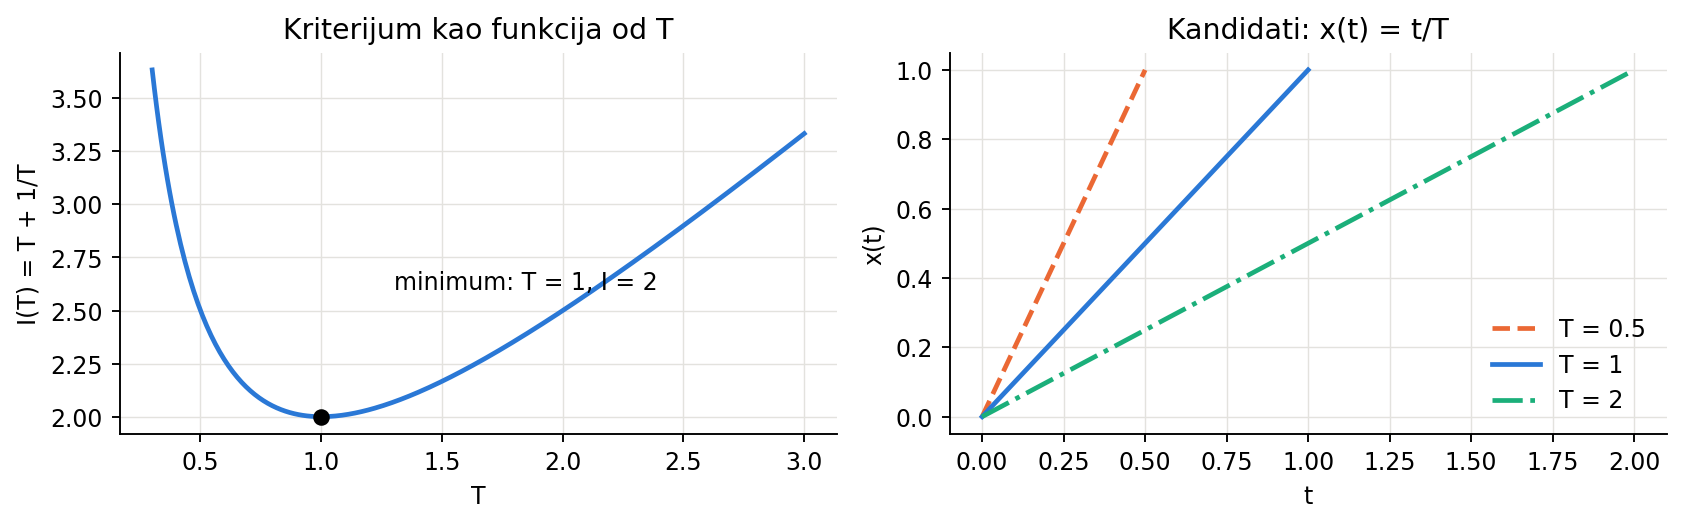
\includegraphics[width=0.85\linewidth,height=\textheight,keepaspectratio,alt={Levo: kriterijum kao funkcija od T, I(T) = T + 1/T, ima minimum baš u T = 1, koje daje uslov H(T) = 0. Desno: kandidati x(t) = t/T. Kratko T traži veliko u (skupo po energiji), a dugo T je skupo po vremenu.}]{figures/q2_primer.png}
\caption{Levo: kriterijum kao funkcija od T, I(T) = T + 1/T, ima minimum baš u T = 1, koje daje uslov H(T) = 0. Desno: kandidati x(t) = t/T. Kratko T traži veliko u (skupo po energiji), a dugo T je skupo po vremenu.}
\end{figure}

Najvažniji primer ovog pitanja je \textbf{problem minimuma vremena} (pitanje 8): tu je \(F = 1\), pa je \(I = T\), a uslov \(H \equiv 0\) služi za određivanje konstanti u \(p(t)\).

\begin{ispit}[{Pitanje 2}]
\begin{itemize}
\item Nacrtati skicu asinhrone varijacije i napisati \(\Delta x = \delta x + \dot x\Delta t\).
\item Pokazati kako se \(-p\delta x - p\dot x\Delta T\) spajaju u \(-p\,\Delta x(T)\). To je ključni korak.
\item Rezultat: \(H(T) = 0\), a za autonoman sistem \(H \equiv 0\). Obavezno prebrojati uslove i nepoznate.
\item Zamka: kad je \(x(T)\) zadato, nula je \(\Delta x(T)\), a ne \(\delta x(T)\).
\end{itemize}
\end{ispit}

\subsection{Moguća potpitanja}

\begin{itemize}
\item \textbf{Zašto je nula \(\Delta x(T)\), a ne \(\delta x(T)\)?} Varirana putanja mora da stigne u \(\beta_i\), ali u trenutku \(T + \Delta T\). Zato je ukupna promena kraja nula, dok je \(\delta x_i(T) = -\dot x_i(T)\Delta T \ne 0\).
\item \textbf{Zašto je \(H \equiv 0\) na celoj putanji, a ne samo u \(T\)?} Za autonoman sistem je \(dH/dt = \partial H/\partial t = 0\), pa je \(H\) konstantno; konstanta je određena sa \(H(T) = 0\).
\item \textbf{Šta ako sistem nije autonoman?} Važi samo \(H(T) = 0\); duž putanje se \(H\) menja po \(dH/dt = \partial H/\partial t\).
\item \textbf{Šta ako je i \(x(T)\) slobodno?} Dodaje se \(p_i(T) = 0\), a \(H(T) = 0\) ostaje. Ako \(\Psi\) zavisi od \(T\), uslov postaje \(H(T) + \partial\Psi/\partial T = 0\) (pitanje 5).
\item \textbf{Šta ako u primeru nema jedinice, \(F = u^2\)?} Tada je \(H = -u^2 = 0\), tj. \(u = 0\): nema konačnog optimalnog \(T\) (sa \(I = 1/T\) uvek se isplati ići sporije). Zato vreme mora biti „kažnjeno'' u \(F\).
\item \textbf{Kako se \(H(T) = 0\) koristi u problemu minimuma vremena?} Daje dodatnu jednačinu koja određuje konstantu u \(p(t)\) (pitanje 8).
\end{itemize}

\section{3. Optimalno upravljanje, Bolcin problem}

\begin{kljucna}[{Odgovor u 60 sekundi}]
\begin{enumerate}
\def\labelenumi{\arabic{enumi}.}
\item Bolcin problem ima kriterijum sa dva dela: \(I = \Psi[T, x(T)] + \int_0^T F\,dt\). Prvi deo ocenjuje samo kraj procesa, drugi ceo tok.
\item \(\Psi\) je „statička'' optimizacija u krajnjoj tački, a integral je dinamička optimizacija; Lagranžov (\(\Psi = 0\)) i Majerov (\(F = 0\)) problem su specijalni slučajevi.
\item Prošireni kriterijum je \(\bar I = \Psi + \int_0^T[H - \sum p_i\dot x_i]dt\), sa istim \(H = F + \sum p_i f_i\).
\item Prva varijacija dobija član \(\sum \frac{\partial\Psi}{\partial x_i(T)}\delta x_i(T)\), koji se sabira sa \(-\sum p_i(T)\delta x_i(T)\) iz parcijalne integracije.
\item Kanonske jednačine se ne menjaju, a menja se granični uslov: \(p_i(T) = \partial\Psi/\partial x_i(T)\).
\item Za \(\Psi = 0\) to je stari uslov \(p_i(T) = 0\). Veliko \(\Psi\) je „meka'' verzija zadatog kraja; tako se kraj uvodi u LQR i u FBSM.
\end{enumerate}
\end{kljucna}

\subsection{Ideja}

Često nas zanima i \textbf{gde} se proces završio, a ne samo koliko je „koštao'' usput. Na primer, kod regulatora želimo da stanje na kraju bude blizu nule, ali ne moramo da ga u nulu dovedemo po svaku cenu. Tada se krajnje stanje ne zadaje tvrdo (\(x(T) = 0\)), nego se kažnjava članom \(\Psi[x(T)]\), npr. \(\frac12\Psi x^2(T)\). Rezultat je samo novi granični uslov za \(p\).

\subsection{Postavka}

\[\dot x_i = f_i(t, x_i, u_k), \qquad x_i(t_0) = \alpha_i, \qquad t_0 \le t \le t_1 \text{ poznato}\]

\[I = \Psi\big[t, x_i(t)\big]\Big|_{t_0}^{t_1} + \int_{t_0}^{t_1} F(t, x_i, u_k)\,dt\]

Ovo je „najsloženiji oblik'': \(\Psi\) može da zavisi i od početka i od kraja. U najčešćem slučaju početak je zadat, pa ostaje samo \(\Psi[T, x_i(T)]\). Dalje se koristi \(t_0 = 0\), \(t_1 = T\).

\textbf{Nazivi} (odeljak „Zajednički alat''): Lagranžov problem je \(\Psi = 0\), Majerov je \(F = 0\), a Bolcin ima oba člana.

\subsection{Izvođenje}

\textbf{Korak 1: prošireni kriterijum.} \(\Psi\) ne sadrži dinamiku, pa ostaje van integrala:

\[\bar I = \Psi\big[T, x_i(T)\big] + \int_0^T\Big[H(t, x_i, u_k, p_i) - \sum_{i=1}^n p_i\dot x_i\Big]dt, \qquad H = F + \sum_{i=1}^n p_i f_i .\]

\textbf{Korak 2: prva varijacija.} \(T\) je poznato. Varijacija člana \(\Psi\) po krajnjem stanju je

\[\delta\Psi = \sum_{i=1}^n \frac{\partial\Psi}{\partial x_i(T)}\,\delta x_i(T) .\]

Integral se varira tačno kao u pitanju 1 (prva varijacija, pa parcijalna integracija člana \(p_i\delta\dot x_i\)). Zajedno:

\[\delta\bar I = \sum_{i=1}^n\frac{\partial\Psi}{\partial x_i(T)}\delta x_i(T) - \sum_{i=1}^n p_i\,\delta x_i\Big|_0^T + \int_0^T\{\dots\}\,dt ,\]

gde je \(\{\dots\}\) isti podintegralni izraz kao u pitanju 1.

\textbf{Korak 3: uslovi pod integralom} su isti kao u pitanju 1: kanonske jednačine i \(\partial H/\partial u_k = 0\) (odeljak „Zajednički alat'').

\textbf{Korak 4: uslov van integrala.} Na početku je \(\delta x_i(0) = 0\). Na kraju se skupe članovi sa \(\delta x_i(T)\):

\[\sum_{i=1}^n\Big[\frac{\partial\Psi}{\partial x_i(T)} - p_i(T)\Big]\delta x_i(T) = 0 .\]

\(x_i(T)\) je slobodno, pa je \(\delta x_i(T)\) proizvoljno i zagrada mora biti nula:

\begin{kljucna}
\[p_i(T) = \frac{\partial\Psi}{\partial x_i(T)}, \qquad i = 1, \dots, n .\]

Ako \(\Psi\) zavisi i od početnog stanja, a \(x_i(0)\) nije zadato, na isti način se dobija \(p_i(0) = \partial\Psi/\partial x_i(0)\) (i \(\Psi\big|_{t_0}^{t_1}\) i \(-p_i\delta x_i\big|_{t_0}^{t_1}\) menjaju znak na donjoj granici, pa uslov \(\big[p_i(t_0) - \partial\Psi/\partial x_i(t_0)\big]\delta x_i(t_0) = 0\) ima isti oblik).
\end{kljucna}

\textbf{Korak 5: veza sa Lagranžovim oblikom.} Bolcin problem se uvek može prevesti u Lagranžov. Pošto je

\[\Psi\big[T, x(T)\big] = \Psi\big[0, x(0)\big] + \int_0^T\frac{d\Psi}{dt}dt = \Psi\big[0, \alpha\big] + \int_0^T\Big(\frac{\partial\Psi}{\partial t} + \sum_i\frac{\partial\Psi}{\partial x_i}f_i\Big)dt,\]

a \(\Psi[0, \alpha]\) je konstanta, isti problem je Lagranžov sa \(F' = F + \partial\Psi/\partial t + \sum_i(\partial\Psi/\partial x_i)f_i\). Isti trik je korišćen u primeru sa robotima na Marsu: Majerov kriterijum \(z(T)\) je napisan kao \(\int_0^T\dot z\,dt\). Zato su tri oblika problema međusobno ekvivalentna, a izbor je stvar zgodnosti.

\textbf{Korak 6: tumačenje.} \(\Psi\) je \textbf{meko} ograničenje na kraj. Primer: \(\Psi = \frac12\Psi_0 x^2(T)\) daje \(p(T) = \Psi_0 x(T)\).

\begin{itemize}
\item \(\Psi_0 = 0\): kraj nas ne zanima, \(p(T) = 0\) (pitanje 1).
\item \(\Psi_0 \to \infty\): svako odstupanje od nule je beskonačno skupo, pa \(x(T) \to 0\). To je granični slučaj \textbf{zadatog} kraja.
\end{itemize}

Na ovome se zasnivaju dve kasnije primene: uslov \(P(T) = \Psi\) za Rikatijevu jednačinu (pitanja 10--12) i uvođenje zadatog kraja kao kazne u FBSM (pitanje 6).

\subsection{\texorpdfstring{Primer: uticaj težine \(\Psi\)}{Primer: uticaj težine \textbackslash Psi}}

\[\dot x = u, \qquad x(0) = 1, \qquad I = \frac12\Psi\,x^2(1) + \frac12\int_0^1 u^2\,dt .\]

\textbf{Uslovi.}

\[H = \tfrac12u^2 + p\,u, \qquad u = -p, \qquad \dot p = -\frac{\partial H}{\partial x} = 0 \;\Rightarrow\; p = \text{const}, \qquad p(1) = \frac{\partial\Psi}{\partial x(1)} = \Psi\,x(1) .\]

\textbf{Rešenje.} \(x(t) = 1 - p\,t\), pa je \(x(1) = 1 - p\). Iz graničnog uslova:

\[p = \Psi(1 - p) \;\Rightarrow\; p = \frac{\Psi}{1 + \Psi}, \qquad u^* = -\frac{\Psi}{1 + \Psi}, \qquad x(1) = \frac{1}{1 + \Psi}, \qquad I_{min} = \frac12\,\frac{\Psi}{1 + \Psi} .\]

\textbf{Provera direktno.} Za konstantno \(u = -c\) je \(I(c) = \frac12\Psi(1 - c)^2 + \frac12c^2\). Izvod \(-\Psi(1 - c) + c = 0\) daje \(c = \Psi/(1 + \Psi)\), isto.

\begin{figure}
\centering
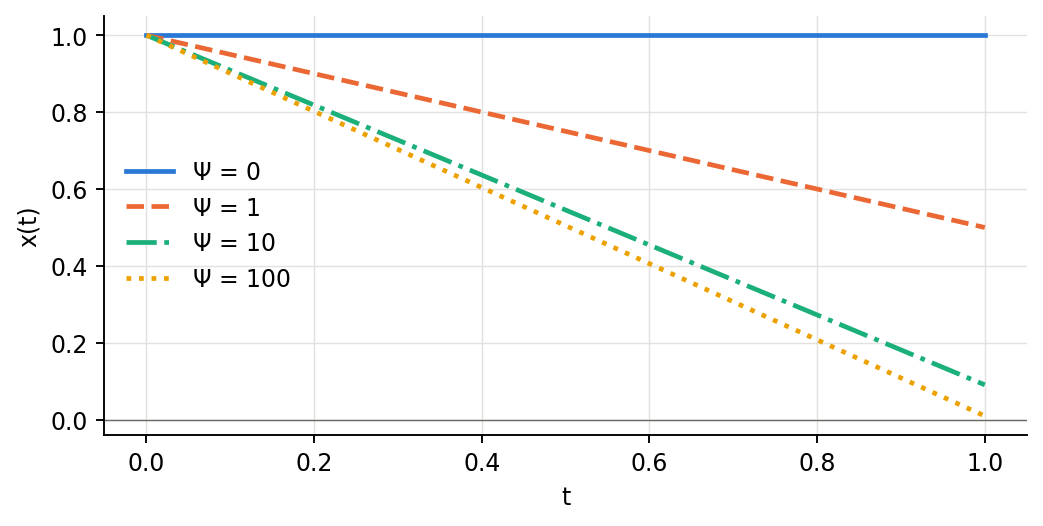
\includegraphics[width=0.7\linewidth,height=\textheight,keepaspectratio,alt={Bolcin problem: optimalno x(t) za razne težine Ψ. Za Ψ = 0 nema kazne za kraj, pa je u = 0 i x ostaje 1. Kako Ψ raste, x(1) = 1/(1 + Ψ) ide ka nuli, tj. ka rešenju sa zadatim krajem x(1) = 0.}]{figures/q3_bolca_psi.png}
\caption{Bolcin problem: optimalno x(t) za razne težine Ψ. Za Ψ = 0 nema kazne za kraj, pa je u = 0 i x ostaje 1. Kako Ψ raste, x(1) = 1/(1 + Ψ) ide ka nuli, tj. ka rešenju sa zadatim krajem x(1) = 0.}
\end{figure}

\begin{ispit}[{Pitanje 3}]
\begin{itemize}
\item Napisati kriterijum \(I = \Psi + \int F\) i reći da je \(\Psi\) statički, a integral dinamički deo.
\item Pokazati kako se \(\frac{\partial\Psi}{\partial x(T)}\delta x(T)\) i \(-p(T)\delta x(T)\) skupljaju u jedan član. Rezultat: \(p_i(T) = \partial\Psi/\partial x_i(T)\).
\item Pomenuti prevođenje Bolca → Lagranž preko \(\Psi(T) = \Psi(0) + \int\dot\Psi\,dt\).
\item Zamka: kanonske jednačine se \textbf{ne menjaju}. Menja se samo granični uslov.
\end{itemize}
\end{ispit}

\subsection{Moguća potpitanja}

\begin{itemize}
\item \textbf{Zašto se kanonske jednačine ne menjaju?} \(\Psi\) zavisi samo od kraja, pa ne ulazi pod integral; koeficijenti uz \(\delta x_i\), \(\delta p_i\), \(\delta u_k\) pod integralom su isti kao u pitanju 1.
\item \textbf{Šta ako je \(x(T)\) zadato, a \(\Psi\) postoji?} Tada je \(\delta x_i(T) = 0\), pa \(\Psi[x(T)]\) je konstanta i ne utiče na rešenje; \(p_i(T)\) ostaje nepoznato, važi \(x_i(T) = \beta_i\).
\item \textbf{Šta ako je i \(T\) slobodno?} Dodaje se uslov \(H(T) + \partial\Psi/\partial T = 0\) (pitanje 5).
\item \textbf{Šta je Majerov problem i kako se rešava?} \(F = 0\), pa je \(H = \sum p_i f_i\), a ceo kriterijum ulazi kroz \(p_i(T) = \partial\Psi/\partial x_i(T)\) (ili se prevede u Lagranžov, korak 5).
\item \textbf{Zašto je veliko \(\Psi\) „meko'' zadat kraj?} Iz primera \(x(1) = 1/(1 + \Psi) \to 0\) kad \(\Psi \to \infty\); za konačno \(\Psi\) kraj je samo blizu nule.
\end{itemize}

\section{4. Optimalno upravljanje, složeni granični problemi}

\begin{kljucna}[{Odgovor u 60 sekundi}]
\begin{enumerate}
\def\labelenumi{\arabic{enumi}.}
\item Složeni granični uslovi: početak i kraj nisu zadati kao tačke, nego kao veze između promenljivih stanja, \(M_\alpha[t_0, x(t_0)] = 0\) (\(s\) veza) i \(N_\beta[t_1, x(t_1)] = 0\) (\(r\) veza), sa \(s, r < n\).
\item Primer: kraj treba da bude bilo gde na pravoj \(x_1 + x_2 = 1\), a ne u jednoj tački.
\item Veze su statička ograničenja u dve tačke, pa se u kriterijum uvode \textbf{konstantnim} Lagranževim množiteljima \(\lambda_\alpha\) i \(\mu_\beta\).
\item Kanonske jednačine su iste kao ranije. Iz članova van integrala dobijaju se uslovi transverzalnosti: \(p_i(t_1) = \partial\Psi/\partial x_i(t_1) + \sum\mu_\beta\,\partial N_\beta/\partial x_i(t_1)\) i isto na početku sa \(\lambda_\alpha\) i \(M_\alpha\).
\item Geometrijski: \(p(t_1)\) je normalan na skup dozvoljenih krajeva.
\item Brojanje: \(2n + r + s\) nepoznatih i isto toliko jednačina.
\end{enumerate}
\end{kljucna}

\subsection{Ideja}

U pitanjima 1--3 kraj je bio ili potpuno zadat, ili potpuno slobodan. Između ta dva slučaja je kraj koji mora da zadovolji \textbf{neke} veze: na primer da leži na nekoj krivoj ili površi (mnogostrukosti). Tada je deo krajnjeg stanja slobodan, a deo nije. Veze se uvode istim trikom kao u statičkoj optimizaciji: Lagranževim množiteljima, ali sada su to konstante, jer veza važi samo u jednom trenutku.

Profesorova formulacija \izvor{P11 snimak, 7.--10. min}: Bolcin član \(\Psi\) i veze \(M_\alpha\), \(N_\beta\) su \textbf{algebarski} izrazi u dve tačke, pa su „u svojoj dubokoj biti deo statičke optimizacije''. Oni se sa kriterijumom spajaju Lagranževim množiteljima, „i to je cela mudrost''.

\subsection{Postavka}

\[\dot x_i = f_i(t, x_i, u_k), \qquad i = 1, \dots, n, \qquad k = 1, \dots, m, \qquad t_0 \le t \le t_1 \text{ poznato}\]

\[M_\alpha\big[t_0, x_i(t_0)\big] = 0, \quad \alpha = 1, \dots, s, \qquad N_\beta\big[t_1, x_i(t_1)\big] = 0, \quad \beta = 1, \dots, r, \qquad s, r < n\]

\[I = \Psi\big[t, x_i(t)\big]\Big|_{t_0}^{t_1} + \int_{t_0}^{t_1}F(t, x_i, u_k)\,dt\]

Između \(t_0\) i \(t_1\) postoji „rigidna (čvrsta) veza'' među promenljivima, i to je ono što uslove čini složenim. Uslov \(s, r < n\) znači da ostaje sloboda za optimizaciju: kad bi bilo \(r = n\) nezavisnih veza, kraj bi bio potpuno određen.

\subsection{Izvođenje}

\textbf{Korak 1: prošireni kriterijum.} Veze \(M_\alpha\) i \(N_\beta\) se dodaju kao u statičkoj optimizaciji, a dinamika kao ranije:

\[\bar I = \Psi\big[t_1, x_i(t_1)\big] + \sum_{\beta=1}^r\mu_\beta N_\beta\big[t_1, x_i(t_1)\big] - \Psi\big[t_0, x_i(t_0)\big] - \sum_{\alpha=1}^s\lambda_\alpha M_\alpha\big[t_0, x_i(t_0)\big] + \int_{t_0}^{t_1}\Big[H - \sum_{i=1}^n p_i\dot x_i\Big]dt .\]

Znak ispred \(\lambda_\alpha\) je izabran tako da krajnji uslovi imaju isti oblik na oba kraja. Pošto je \(\lambda_\alpha\) nepoznata konstanta proizvoljnog znaka, ovaj izbor ne menja rezultat.

\textbf{Korak 2: prva varijacija.} Sada su slobodni i \(\delta x_i(t_0)\) i \(\delta x_i(t_1)\). Integral se varira kao u pitanju 1, a članovi van integrala se diferenciraju po krajnjim stanjima:

\[
\begin{aligned}
\delta\bar I ={}& \sum_{i=1}^n\Big[\frac{\partial\Psi}{\partial x_i(t_1)} + \sum_{\beta=1}^r\mu_\beta\frac{\partial N_\beta}{\partial x_i(t_1)} - p_i(t_1)\Big]\delta x_i(t_1) \\
&- \sum_{i=1}^n\Big[\frac{\partial\Psi}{\partial x_i(t_0)} + \sum_{\alpha=1}^s\lambda_\alpha\frac{\partial M_\alpha}{\partial x_i(t_0)} - p_i(t_0)\Big]\delta x_i(t_0) \\
&+ \int_{t_0}^{t_1}\{\dots\}\,dt = 0 .
\end{aligned}
\]

Podintegralni izraz \(\{\dots\}\) je isti kao u pitanju 1. Članovi \(-p_i(t_1)\delta x_i(t_1)\) i \(+p_i(t_0)\delta x_i(t_0)\) potiču od \(-\sum p_i\delta x_i\big|_{t_0}^{t_1}\) iz parcijalne integracije.

\textbf{Korak 3: uslovi pod integralom} su kanonske jednačine i \(\partial H/\partial u_k = 0\), kao u pitanju 1 (\(2n\) diferencijalnih i \(m\) algebarskih jednačina; odeljak „Zajednički alat'').

\textbf{Korak 4: uslovi transverzalnosti.} Pošto su množitelji uvedeni, \(\delta x_i(t_0)\) i \(\delta x_i(t_1)\) se mogu smatrati nezavisnim, pa su obe zagrade nula. (Isti argument kao u statičkoj optimizaciji: zbog \(r\) veza samo \(n - r\) komponenti \(\delta x(t_1)\) je slobodno; \(r\) množitelja \(\mu_\beta\) se biraju tako da ponište koeficijente uz preostalih \(r\) zavisnih komponenti.)

\begin{kljucna}
\[p_i(t_1) = \frac{\partial\Psi}{\partial x_i(t_1)} + \sum_{\beta=1}^r\mu_\beta\frac{\partial N_\beta}{\partial x_i(t_1)}, \qquad p_i(t_0) = \frac{\partial\Psi}{\partial x_i(t_0)} + \sum_{\alpha=1}^s\lambda_\alpha\frac{\partial M_\alpha}{\partial x_i(t_0)}\]

uz same veze \(M_\alpha[t_0, x(t_0)] = 0\) i \(N_\beta[t_1, x(t_1)] = 0\).
\end{kljucna}

\textbf{Korak 5: brojanje.} Nepoznate su: \(2n\) konstanti integracije, \(r\) množitelja \(\mu_\beta\) i \(s\) množitelja \(\lambda_\alpha\), ukupno \(2n + r + s\). Jednačine su: \(n\) uslova za \(p_i(t_0)\), \(s\) veza \(M_\alpha = 0\), \(n\) uslova za \(p_i(t_1)\) i \(r\) veza \(N_\beta = 0\), ukupno \(2n + r + s\). Broj se slaže.

\textbf{Korak 6: provera na poznatim slučajevima.}

\begin{itemize}
\item \textbf{Zadat početak} \(x_i(t_0) = \alpha_i\) je specijalan slučaj \(M_i = x_i(t_0) - \alpha_i\), \(s = n\). Tada je \(p_i(t_0) = \lambda_i\), a \(\lambda_i\) je slobodna nepoznata: uslov za \(p_i(t_0)\) ne postoji, ostaje samo \(x_i(t_0) = \alpha_i\). To je upravo pitanje 1.
\item \textbf{Zadat kraj} \(N_i = x_i(t_1) - \beta_i\): \(p_i(t_1) = \mu_i\) je nepoznato. Isto kao u pitanju 1.
\item \textbf{Slobodan kraj} (\(r = 0\)): \(p_i(t_1) = \partial\Psi/\partial x_i(t_1)\), tj. pitanje 3.
\end{itemize}

\textbf{Korak 7: geometrijsko tumačenje.} Za \(\Psi = 0\) je \(p(t_1) = \sum\mu_\beta\nabla N_\beta\), a gradijent \(\nabla N_\beta\) je normalan na površ \(N_\beta = 0\). Znači: \textbf{vektor \(p(t_1)\) je normalan na skup dozvoljenih krajeva}. Duž te površi kriterijum više ne može da se smanji, pa „cena'' pomeranja kraja ima samo normalnu komponentu.

\textbf{Kako se rešava.} Na snimku profesor kaže: „Ovde imamo kombinaciju dinamičke i statičke optimizacije. Dinamička se odnosi na sve što se dešava u intervalu između \(t_0\) i \(t_1\), a u tačkama \(t_0\) i \(t_1\) radimo statičku optimizaciju'' \izvor{P11 snimak, 26. min}. Iz dinamičkog dela dolaze kanonske jednačine, a iz statičkog uslovi za \(p(t_0)\), \(p(t_1)\) i same veze. (Skica „podeljenog intervala'' iz beleški sa časa verovatno prikazuje baš ovu podelu, a ne diskretizaciju.) Numerički se rešava kao dvotačkasti problem (pitanje 6), sa dodatnim nepoznatim \(\mu\) i \(\lambda\).

\subsection{Primer: kraj na pravoj}

\[\dot x_1 = x_2, \qquad \dot x_2 = u, \qquad x(0) = (0, 0), \qquad T = 1, \qquad N = x_1(1) + x_2(1) - 1 = 0, \qquad I = \frac12\int_0^1u^2\,dt .\]

Pozicija i brzina na kraju nisu zadate pojedinačno, zadat je samo njihov zbir.

\textbf{Hamiltonijan i kanonske jednačine.}

\[H = \tfrac12u^2 + p_1x_2 + p_2u, \qquad u = -p_2, \qquad \dot p_1 = 0, \qquad \dot p_2 = -p_1 .\]

\textbf{Transverzalnost} (\(\Psi = 0\), \(\nabla N = (1, 1)\)): \(p_1(1) = \mu\), \(p_2(1) = \mu\).

\textbf{Rešavanje.} \(p_1 = \mu\) (konstanta), pa je \(p_2(t) = p_2(1) + \mu(1 - t) = \mu(2 - t)\). Upravljanje je \(u = -\mu(2 - t)\). Integracijom od nule:

\[x_2(t) = -\mu\Big(2t - \frac{t^2}{2}\Big), \qquad x_1(t) = -\mu\Big(t^2 - \frac{t^3}{6}\Big) .\]

U \(t = 1\): \(x_2(1) = -\frac32\mu\), \(x_1(1) = -\frac56\mu\). Iz veze \(N = 0\):

\[-\frac56\mu - \frac32\mu = 1 \;\Rightarrow\; -\frac{14}{6}\mu = 1 \;\Rightarrow\; \mu = -\frac37 .\]

\[u^*(t) = \frac37(2 - t), \qquad x(1) = \Big(\frac{5}{14}, \frac{9}{14}\Big) = (0{,}357;\ 0{,}643), \qquad I_{min} = \frac12\int_0^1\frac{9}{49}(2 - t)^2dt = \frac{3}{14} = 0{,}214 .\]

Provera: \(0{,}357 + 0{,}643 = 1\). Brojanje: nepoznate su 4 konstante i \(\mu\) (5), a uslovi su \(x(0) = 0\) (2), dva uslova transverzalnosti i \(N = 0\) (3).

\begin{figure}
\centering
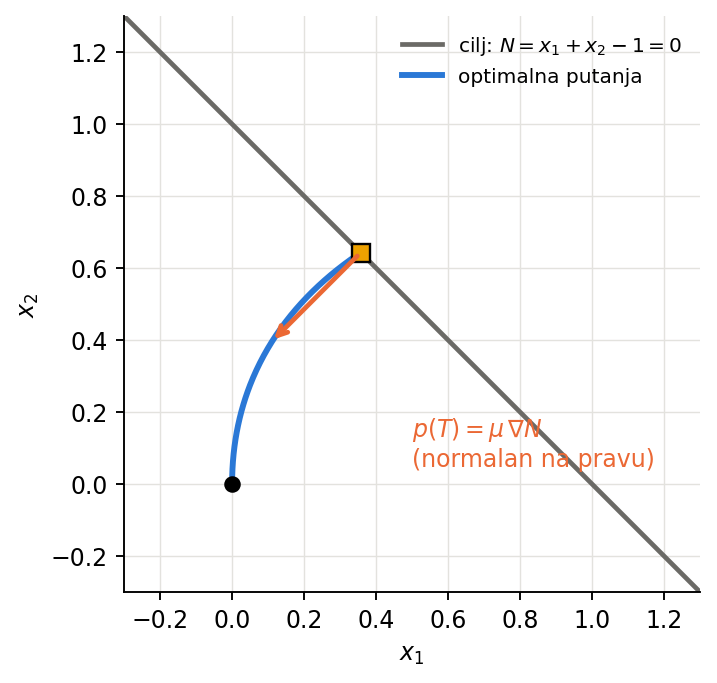
\includegraphics[width=0.6\linewidth,height=\textheight,keepaspectratio,alt={Kraj na mnogostrukosti. Optimalna putanja u faznoj ravni polazi iz nule i završava na pravoj x₁ + x₂ = 1. Strelica je p(T) = μ∇N: normalna je na pravu, kako tvrdi uslov transverzalnosti.}]{figures/q4_mnogostrukost.png}
\caption{Kraj na mnogostrukosti. Optimalna putanja u faznoj ravni polazi iz nule i završava na pravoj x₁ + x₂ = 1. Strelica je p(T) = μ∇N: normalna je na pravu, kako tvrdi uslov transverzalnosti.}
\end{figure}

\begin{ispit}[{Pitanje 4}]
\begin{itemize}
\item Definisati \(M_\alpha\), \(N_\beta\), objasniti \(s, r < n\) i napisati prošireni kriterijum sa \(\lambda_\alpha\) i \(\mu_\beta\).
\item Rezultat: dva uslova transverzalnosti (za \(p(t_0)\) i \(p(t_1)\)) i prebrojavanje \(2n + r + s\).
\item Pokazati da su zadat i slobodan kraj specijalni slučajevi. To pokazuje razumevanje.
\item Zamka: \(\lambda_\alpha\) i \(\mu_\beta\) su \textbf{konstante} (statički množitelji), a \(p_i(t)\) su funkcije vremena.
\end{itemize}
\end{ispit}

\subsection{Moguća potpitanja}

\begin{itemize}
\item \textbf{Zašto su \(\mu_\beta\) i \(\lambda_\alpha\) konstante, a \(p_i\) funkcije?} Veze \(N_\beta\), \(M_\alpha\) važe samo u jednom trenutku (po jedna jednačina), a dinamika važi u svakom \(t\).
\item \textbf{Uvedeni su množitelji, odakle jednačine za njih?} Izvod proširenog kriterijuma po \(\lambda_\alpha\) i \(\mu_\beta\) daje same veze \(M_\alpha = 0\) i \(N_\beta = 0\), kao u statičkoj optimizaciji \izvor{P11 snimak, 24. min}.
\item \textbf{Da li je bitan znak ispred množitelja?} Nije. Kod ograničenja tipa jednakosti znak menja samo znak dobijenog \(\lambda\); minus je izabran jer je kasnije lakše \izvor{P11 snimak, 10. min}.
\item \textbf{Zašto je \(s, r < n\)?} Za \(r = n\) nezavisnih veza kraj je jedna tačka (zadat kraj, pitanje 1); za \(r > n\) problem je u opštem slučaju nerešiv.
\item \textbf{Šta znači da je \(p(t_1)\) normalno na mnogostrukost?} Za \(\Psi = 0\) je \(p(t_1) = \sum\mu_\beta\nabla N_\beta\); pomeranje kraja duž površi ne menja kriterijum u prvom redu, pa \(p\) nema tangencijalnu komponentu.
\item \textbf{Kako iz ovoga dobiti pitanje 1?} \(N_i = x_i(t_1) - \beta_i\) (\(r = n\)) daje \(p_i(t_1) = \mu_i\) nepoznato, ostaje \(x_i(t_1) = \beta_i\); \(r = 0\) daje \(p_i(t_1) = \partial\Psi/\partial x_i\) (pitanje 3).
\item \textbf{Šta ako je i \(t_1\) slobodno?} Dodaje se \(H(t_1) + \partial\Psi/\partial t_1 + \sum\mu_\beta\,\partial N_\beta/\partial t_1 = 0\) (pitanje 5).
\end{itemize}

\section{5. Optimalno upravljanje, Bolcin problem, složeni granični uslovi, nespecificirani vremenski interval}

\begin{kljucna}[{Odgovor u 60 sekundi}]
\begin{enumerate}
\def\labelenumi{\arabic{enumi}.}
\item Ovo je najopštiji slučaj: kriterijum \(I = \Psi[T, x(T)] + \int_0^T F\,dt\) (Bolca), kraj na mnogostrukosti \(N_\beta[T, x(T)] = 0\) (složeni uslovi) i nepoznato \(T\).
\item Prošireni kriterijum: \(\bar I = \Psi + \sum\mu_\beta N_\beta + \int_0^T[H - \sum p_i\dot x_i]dt\).
\item Pošto je \(T\) nepoznato, koristi se asinhrona varijacija: \(\Delta x = \delta x + \dot x\Delta T\), i integral dobija član \([H - \sum p_i\dot x_i]\Delta T\).
\item Članovi \(-p\,\delta x(T)\) i \(-p\,\dot x\,\Delta T\) se spajaju u \(-p\,\Delta x(T)\), pa ostaju dva nezavisna koeficijenta: uz \(\Delta x_i(T)\) i uz \(\Delta T\).
\item Rezultat: \(p_i(T) = \partial\Psi/\partial x_i(T) + \sum\mu_\beta\,\partial N_\beta/\partial x_i(T)\) i \(\partial\Psi/\partial T + \sum\mu_\beta\,\partial N_\beta/\partial T + H(T) = 0\).
\item Sva prethodna pitanja (1--4) su specijalni slučajevi ovih uslova.
\end{enumerate}
\end{kljucna}

\subsection{Ideja}

Pitanja 2, 3 i 4 su dodavala po jedno uopštenje: nepoznato \(T\), član \(\Psi\) i veze na kraju. Ovde se sva tri uključuju odjednom. Izvođenje je spoj ta tri izvođenja i ne donosi ništa novo, osim što se Lagranževi množitelji i asinhrona varijacija pojavljuju zajedno. Zato je ovo pitanje dobra prilika da se pokaže da se razume \textbf{odakle} dolazi svaki član.

\subsection{Postavka}

\[\dot x_i = f_i(t, x_i, u_k), \qquad i = 1, \dots, n, \qquad k = 1, \dots, m, \qquad x_i(0) = \alpha_i \text{ poznato}, \qquad T = \;?\]

\[I = \Psi\big[T, x_i(T)\big] + \int_0^T F(t, x_i, u_k)\,dt, \qquad N_\beta\big[T, x_i(T)\big] = 0, \quad \beta = 1, \dots, r\]

Profesor ovo zove „najopštiji slučaj''.

\subsection{Izvođenje}

\textbf{Korak 1: prošireni kriterijum.}

\[\bar I = \Psi\big[T, x_i(T)\big] + \sum_{\beta=1}^r\mu_\beta N_\beta\big[T, x_i(T)\big] + \int_0^T\Big[H(t, x_i, u_k, p_i) - \sum_{i=1}^n p_i\dot x_i\Big]dt, \qquad H = F + \sum_{i=1}^n p_i f_i .\]

\textbf{Korak 2: varijacija članova van integrala.} \(\Psi\) i \(N_\beta\) zavise od \(T\) i od \(x(T)\), a obe veličine se menjaju. Zato se diferenciraju po oba argumenta, sa \textbf{ukupnom} promenom stanja \(\Delta x_i(T)\):

\[\Delta\Big(\Psi + \sum_\beta\mu_\beta N_\beta\Big) = \sum_{i=1}^n\Big[\frac{\partial\Psi}{\partial x_i(T)} + \sum_{\beta=1}^r\mu_\beta\frac{\partial N_\beta}{\partial x_i(T)}\Big]\Delta x_i(T) + \Big[\frac{\partial\Psi}{\partial T} + \sum_{\beta=1}^r\mu_\beta\frac{\partial N_\beta}{\partial T}\Big]\Delta T .\]

\textbf{Korak 3: varijacija integrala.} Kao u pitanju 2, sa \(G = H - \sum p_i\dot x_i\):

\[\Delta\int_0^T G\,dt = \delta\int_0^T G\,dt + G(T)\,\Delta T,\]

a sinhroni deo je kao u pitanju 1 (parcijalna integracija): \(\delta\int_0^T G\,dt = -\sum_i p_i\,\delta x_i\big|_0^T + \int_0^T\{\dots\}\,dt\), sa istim podintegralnim izrazom kao u pitanju 1.

\textbf{Korak 4: spajanje.} Na početku je \(\delta x_i(0) = 0\) jer je \(x_i(0) = \alpha_i\). Na kraju se, kao u pitanju 2, spajaju

\[-\sum_i p_i(T)\,\delta x_i(T) - \sum_i p_i(T)\,\dot x_i(T)\,\Delta T = -\sum_i p_i(T)\,\Delta x_i(T),\]

a od \(G(T)\Delta T\) ostaje samo \(H(T)\Delta T\). Ukupno:

\[\Delta\bar I = \sum_{i=1}^n\Big[\frac{\partial\Psi}{\partial x_i(T)} + \sum_{\beta}\mu_\beta\frac{\partial N_\beta}{\partial x_i(T)} - p_i(T)\Big]\Delta x_i(T) + \Big[\frac{\partial\Psi}{\partial T} + \sum_{\beta}\mu_\beta\frac{\partial N_\beta}{\partial T} + H(T)\Big]\Delta T + \int_0^T\{\dots\}\,dt = 0 .\]

\textbf{Korak 5: uslovi.} \(\Delta x_i(T)\) i \(\Delta T\) se posle uvođenja \(\mu_\beta\) mogu smatrati nezavisnim i proizvoljnim, pa je svaka zagrada nula.

\begin{kljucna}
Kanonske jednačine: \(\dot x_i = \partial H/\partial p_i\), \(\dot p_i = -\partial H/\partial x_i\), \(\partial H/\partial u_k = 0\).

\[p_i(T) = \frac{\partial\Psi}{\partial x_i(T)} + \sum_{\beta=1}^r\mu_\beta\frac{\partial N_\beta}{\partial x_i(T)}, \qquad \frac{\partial\Psi}{\partial T} + \sum_{\beta=1}^r\mu_\beta\frac{\partial N_\beta}{\partial T} + H(T) = 0\]

uz \(x_i(0) = \alpha_i\) i \(N_\beta[T, x(T)] = 0\).
\end{kljucna}

\textbf{Korak 6: brojanje.} Nepoznate: \(2n\) konstanti, \(r\) množitelja \(\mu_\beta\) i \(T\), ukupno \(2n + r + 1\). Jednačine: \(n\) početnih uslova, \(n\) uslova za \(p_i(T)\), \(r\) veza \(N_\beta = 0\) i jedan uslov za \(T\), ukupno \(2n + r + 1\).

\textbf{Korak 7: specijalni slučajevi.}

\begin{longtable}[]{@{}
  >{\raggedright\arraybackslash}p{(\linewidth - 4\tabcolsep) * \real{0.3077}}
  >{\raggedright\arraybackslash}p{(\linewidth - 4\tabcolsep) * \real{0.3077}}
  >{\centering\arraybackslash}p{(\linewidth - 4\tabcolsep) * \real{0.3846}}@{}}
\caption{Pitanja 1--4 kao specijalni slučajevi pitanja 5}\tabularnewline
\toprule\noalign{}
\begin{minipage}[b]{\linewidth}\raggedright
Slučaj
\end{minipage} & \begin{minipage}[b]{\linewidth}\raggedright
Šta se dobija iz opštih uslova
\end{minipage} & \begin{minipage}[b]{\linewidth}\centering
Pitanje
\end{minipage} \\
\midrule\noalign{}
\endfirsthead
\toprule\noalign{}
\begin{minipage}[b]{\linewidth}\raggedright
Slučaj
\end{minipage} & \begin{minipage}[b]{\linewidth}\raggedright
Šta se dobija iz opštih uslova
\end{minipage} & \begin{minipage}[b]{\linewidth}\centering
Pitanje
\end{minipage} \\
\midrule\noalign{}
\endhead
\bottomrule\noalign{}
\endlastfoot
\(\Psi = 0\), nema \(N\), \(T\) poznato & \(p_i(T) = 0\) & 1 \\
\(\Psi = 0\), \(N_i = x_i(T) - \beta_i\), \(T\) nepoznato & \(p_i(T) = \mu_i\) (nepoznato), \(H(T) = 0\) & 2 \\
\(\Psi \ne 0\), nema \(N\), \(T\) poznato & \(p_i(T) = \partial\Psi/\partial x_i(T)\) & 3 \\
\(\Psi\) i \(N\), \(T\) poznato & \(p_i(T) = \partial\Psi/\partial x_i + \sum\mu_\beta\partial N_\beta/\partial x_i\) & 4 \\
\end{longtable}

Kad je \(T\) poznato, \(\Delta T = 0\), pa uslov za \(T\) otpada.

\subsection{Primer: presretanje pokretne mete}

Tačka \(x\) kreće iz nule i treba da stigne metu koja se kreće po zakonu \(g(t) = 1 + t/2\). Kažnjava se i vreme i energija, a vreme presretanja nije zadato:

\[\dot x = u, \qquad x(0) = 0, \qquad I = \underbrace{T}_{\Psi} + \frac12\int_0^T u^2\,dt, \qquad N = x(T) - 1 - \frac T2 = 0, \qquad T = \;?\]

Tu su sva tri elementa: \(\Psi = T\) (Bolca), veza \(N\) koja zavisi i od \(x(T)\) i od \(T\) (složen uslov) i nepoznato \(T\).

\textbf{Kanonske jednačine.}

\[H = \tfrac12u^2 + p\,u, \qquad u = -p, \qquad \dot p = -\frac{\partial H}{\partial x} = 0 \;\Rightarrow\; p = \text{const} .\]

\textbf{Uslov za \(p(T)\).} \(\partial\Psi/\partial x(T) = 0\), \(\partial N/\partial x(T) = 1\), pa je \(p(T) = \mu\). Znači \(p \equiv \mu\) i \(u \equiv -\mu\).

\textbf{Uslov za \(T\).} \(\partial\Psi/\partial T = 1\), \(\partial N/\partial T = -\frac12\), \(H = \frac12\mu^2 - \mu^2 = -\frac12\mu^2\):

\[1 - \frac\mu2 - \frac{\mu^2}{2} = 0 \;\Rightarrow\; \mu^2 + \mu - 2 = 0 \;\Rightarrow\; \mu = -2 \;\text{ ili }\; \mu = 1 .\]

Za \(\mu = 1\) je \(u = -1\), pa \(x = -t\) nikad ne stiže metu koja je iznad 1. Ostaje \(\mu = -2\), \(u^* = 2\), \(x^*(t) = 2t\).

\textbf{Vreme presretanja} iz \(N = 0\): \(2T = 1 + T/2\), pa je \(T = 2/3\). Vrednost: \(I = \frac23 + \frac12\cdot4\cdot\frac23 = 2\).

\textbf{Provera direktno.} Za zadato \(T\) najbolje je konstantno \(u = (1 + T/2)/T\), pa je \(I(T) = T + \frac{(1 + T/2)^2}{2T} = \frac98T + \frac{1}{2T} + \frac12\). Izvod \(\frac98 - \frac{1}{2T^2} = 0\) daje \(T = 2/3\) i \(I = 2\).

\begin{figure}
\centering
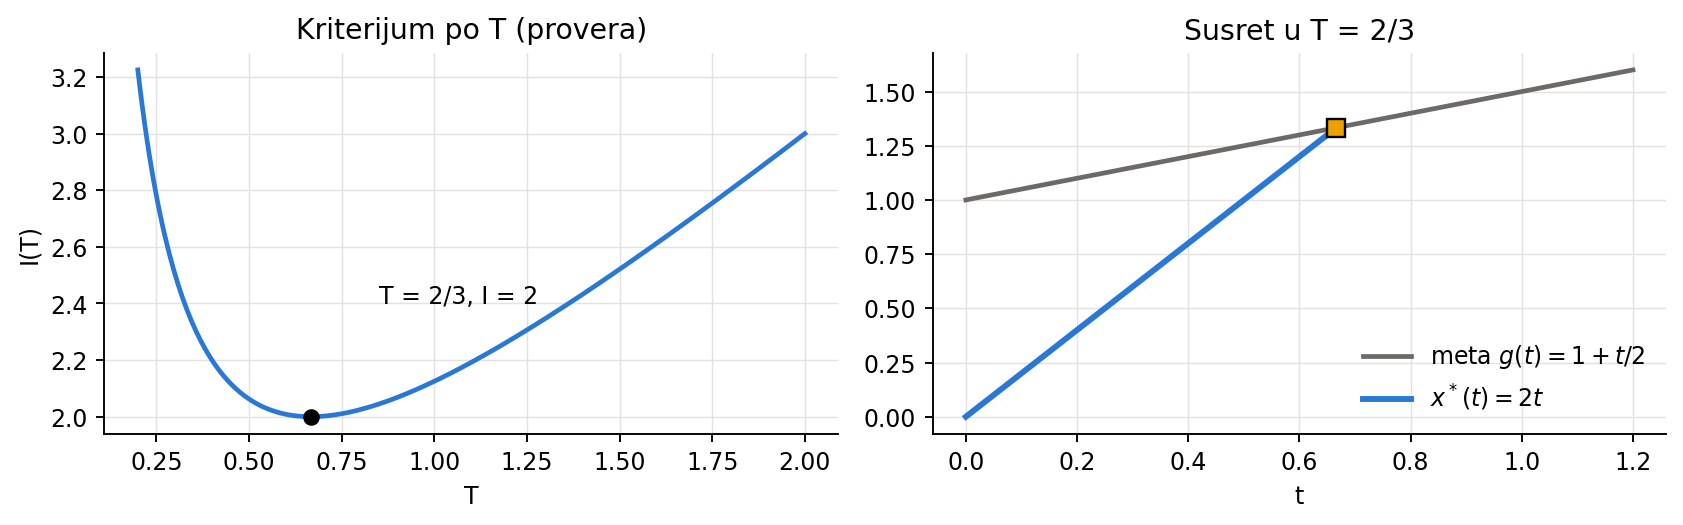
\includegraphics[width=0.85\linewidth,height=\textheight,keepaspectratio,alt={Presretanje pokretne mete. Levo: kriterijum kao funkcija od T ima minimum u T = 2/3, koji su dali uslovi transverzalnosti. Desno: optimalna putanja x* = 2t stiže metu g(t) = 1 + t/2 u T = 2/3.}]{figures/q5_meta.png}
\caption{Presretanje pokretne mete. Levo: kriterijum kao funkcija od T ima minimum u T = 2/3, koji su dali uslovi transverzalnosti. Desno: optimalna putanja x* = 2t stiže metu g(t) = 1 + t/2 u T = 2/3.}
\end{figure}

\begin{ispit}[{Pitanje 5}]
\begin{itemize}
\item Profesor: „Ovo je najopštiji slučaj. Iz njega se mogu izvesti apsolutno svi primeri do sada. Ako znate da rešite ovaj, znate da rešite sve'' \izvor{P11 snimak, 35. min}. Granične uslove na času traži da student sam izvede iz varijacije.
\item Potreban uslov je da je \textbf{asinhrona} varijacija nula (jer je \(T\) nepoznato). \(H(T) = 0\) nije opšti uslov, nego rezultat posebnog slučaja iz pitanja 2.
\item Početi od najopštije postavke, pa izvesti uslove spajanjem koraka iz pitanja 2, 3 i 4. Ne treba ponavljati parcijalnu integraciju do detalja, ali treba reći odakle dolazi \(-\sum p_i\delta x_i|_0^T\).
\item Ključni korak: \(\Psi\) i \(N\) se diferenciraju po \(\Delta x(T)\) i po \(\Delta T\); \(-p\delta x - p\dot x\Delta T = -p\Delta x\).
\item Završiti tabelom specijalnih slučajeva: pokazuje da je ovo opšta teorema.
\item Zamka: u uslovu za \(T\) je \(H(T)\) sa \textbf{plusom}, uz \(\partial\Psi/\partial T\) i \(\mu\,\partial N/\partial T\).
\end{itemize}
\end{ispit}

\subsection{Moguća potpitanja}

\begin{itemize}
\item \textbf{Zašto se \(\Psi\) i \(N\) diferenciraju po \(\Delta x(T)\), a ne po \(\delta x(T)\)?} Oni zavise od stvarnog krajnjeg stanja, a ono se u variranoj putanji menja za ukupnu promenu \(\Delta x = \delta x + \dot x\Delta T\).
\item \textbf{Odakle \(H(T)\) sa plusom?} Iz člana \(G(T)\Delta T = [H - \sum p_i\dot x_i]_T\Delta T\); deo \(-\sum p_i\dot x_i\Delta T\) ode u \(-p\,\Delta x(T)\), a ostaje \(+H(T)\Delta T\).
\item \textbf{Kako se dobija problem minimuma vremena?} \(F = 1\), \(\Psi = 0\), \(N_i = x_i(T) - \beta_i\): \(p_i(T) = \mu_i\) nepoznato, a uslov za \(T\) je \(H(T) = 0\) (pitanja 2 i 8).
\item \textbf{Zašto je u primeru odbačeno \(\mu = 1\)?} Obe vrednosti zadovoljavaju potrebne uslove, ali za \(\mu = 1\) je \(x = -t\) i veza \(N = 0\) nema rešenje sa \(T > 0\). Potrebni uslovi daju kandidate; bira se onaj koji je dopustiv (i daje manji \(I\)).
\item \textbf{Koliko ima uslova?} \(2n + r + 1\) nepoznatih (\(2n\) konstanti, \(\mu_\beta\), \(T\)) i isto toliko jednačina (korak 6).
\end{itemize}

\section{6. Numeričko rešenje: sistem drugog reda, kvadratni kriterijum (ẍ − x = u)}

Zvaničan tekst: \emph{Numerički izračunati optimalnu strategiju upravljanja i kretanje u prostoru stanja. Proces je opisan diferencijalnom jednačinom \(\ddot x - x = u\), uz početne uslove \(x(0) = 1\). Kriterijum optimalnosti je \(I = \int_0^1 u^2(t)\,dt\).} \izvor{zadatak 6}

\begin{kljucna}[{Odgovor u 60 sekundi}]
\begin{enumerate}
\def\labelenumi{\arabic{enumi}.}
\item Stanja \(x_1 = x\), \(x_2 = \dot x\): \(\dot x_1 = x_2\), \(\dot x_2 = x_1 + u\). Sistem je nestabilan (polovi \(\pm1\)).
\item Tekst zadaje samo \(x(0) = 1\). Sa slobodnim krajem je \(p(1) = 0\), pa \(p \equiv 0\) i \(u \equiv 0\): trivijalno. Zato se uzima problem minimuma energije: \((1, 0) \to (0, 0)\) za \(T = 1\).
\item \(H = u^2 + p_1x_2 + p_2(x_1 + u)\); \(u\) nije ograničeno, pa \(u^* = -p_2/2\); \(\dot p_1 = -p_2\), \(\dot p_2 = -p_1\).
\item To je dvotačkasti problem: 4 jednačine, \(x\) zadato na oba kraja, \(p\) nigde.
\item Numerički: \texttt{bvp4c} direktno, ili FBSM sa vežbi, gde se kraj uvodi kao kazna \(\Psi\|x(1)\|^2\) (Bolca), pa je \(p(1) = 2\Psi x(1)\), a \(\Psi\) se povećava.
\item Rezultat: \(u^*\) raste od \(-7{,}25\) do \(+6{,}17\), \(I_{min} = 14{,}765\); FBSM teži tome kad \(\Psi \to \infty\).
\end{enumerate}
\end{kljucna}

\subsection{Ideja}

Treba „prevesti'' nestabilan sistem iz mirovanja u tački 1 u mirovanje u nuli sa najmanje energije (\(\int u^2\)). Kriterijum je kvadratan po \(u\), pa je upravljanje glatko (nije relejno) i dobija se iz \(\partial H/\partial u = 0\). Teškoća nije u izvođenju, nego u tome što je \(x\) zadato na oba kraja, a \(p\) ni na jednom. Zato se problem rešava numerički, iterativno.

\subsection{Postavka i granični uslovi}

Prostor stanja (\(x_1 = x\), \(x_2 = \dot x\)):

\[\dot x_1 = x_2, \qquad \dot x_2 = x_1 + u, \qquad I = \int_0^1 u^2\,dt .\]

\textbf{Problem sa tekstom.} Sistem je drugog reda, pa dvotačkasti problem traži 4 uslova, a zadat je samo \(x(0) = 1\). Ako je sve ostalo slobodno, uslovi transverzalnosti su \(p_1(1) = p_2(1) = 0\). Adjungovane jednačine (ispod) ne zavise od \(x\) ni od \(u\), pa je tada \(p \equiv 0\), \(u \equiv 0\) i \(I = 0\): najjeftinije je ne raditi ništa, jer se plaća samo upravljanje. Tada \(x(t) = \cosh t\) „pobegne'' do \(x(1) = 1{,}543\) (provereno numerički).

\textbf{Usvojeno:} problem minimuma energije

\[x(0) = 1, \quad \dot x(0) = 0 \quad\longrightarrow\quad x(1) = 0, \quad \dot x(1) = 0 .\]

Na ispitu treba reći ovu dilemu naglas i objasniti izbor. Ako se uzme \(x(0) = 1\), \(\dot x(0) = 1\) i slobodan kraj, tačan rezultat je \(u \equiv 0\). Česta greška: u iteraciji za \(p_2\) napisati \(T_s\cdot T_s\) umesto \(T_s\), pa iteracija to ne pokaže jasno.

\subsection{Izvođenje uslova}

\[H = u^2 + p_1x_2 + p_2(x_1 + u)\]

\[\frac{\partial H}{\partial u} = 2u + p_2 = 0 \;\Rightarrow\; u^* = -\frac{p_2}{2}, \qquad \frac{\partial^2H}{\partial u^2} = 2 > 0 \;(\text{minimum})\]

\[\dot p_1 = -\frac{\partial H}{\partial x_1} = -p_2, \qquad \dot p_2 = -\frac{\partial H}{\partial x_2} = -p_1 .\]

Diferenciranjem: \(\ddot p_2 = -\dot p_1 = p_2\), pa je \(p_2 = c_1e^t + c_2e^{-t}\). Adjungovani sistem ima iste modove kao proces (\(\pm1\)). Zato je i \(u^*\) linearna kombinacija \(e^t\) i \(e^{-t}\).

\textbf{Dvotačkasti problem:}

\[\dot x_1 = x_2, \quad \dot x_2 = x_1 - \frac{p_2}{2}, \quad \dot p_1 = -p_2, \quad \dot p_2 = -p_1, \qquad x(0) = (1, 0), \quad x(1) = (0, 0) .\]

\subsection{Analitička kontrola}

Za proveru numerike vredi znati i tačno rešenje. Neka je \(u = Ae^t + Be^{-t}\). Jednačina \(\ddot x - x = u\) ima rezonancu (desna strana ima iste eksponente kao homogeno rešenje), pa je partikularno rešenje oblika \(t\,e^{\pm t}\):

\[x(t) = C\cosh t + D\sinh t + \frac A2\,t\,e^t - \frac B2\,t\,e^{-t} .\]

(Provera: za \(x_p = \frac A2te^t\) je \(\ddot x_p - x_p = Ae^t\).) Četiri uslova \(x(0) = 1\), \(\dot x(0) = 0\), \(x(1) = 0\), \(\dot x(1) = 0\) daju linearni sistem za \(A, B, C, D\):

\[A = 3{,}7584, \qquad B = -11{,}0064, \qquad C = 1, \qquad D = -7{,}3824\]

\[u^*(t) = 3{,}7584\,e^t - 11{,}0064\,e^{-t}, \qquad u(0) = -7{,}25, \qquad u(1) = 6{,}17, \qquad I_{min} = 14{,}765 .\]

Isti broj daje formula za minimum energije preko Gramijana upravljivosti, \(I_{min} = (e^{AT}x_0)^TW^{-1}(e^{AT}x_0)\), \(W = \int_0^Te^{A\tau}BB^Te^{A^T\tau}d\tau\). Iz \(p_2 = -2u\) i \(p_1 = -\dot p_2\) sledi \(p(0) = (29{,}53;\ 14{,}50)\).

\subsection{Numerički postupak 1: rešavač graničnog problema}

MATLAB \texttt{bvp4c} (ili Python \texttt{solve\_bvp}) direktno rešava 4 jednačine sa 2 uslova na početku i 2 na kraju. Dobija se \(I = 14{,}7649\) i \(p(0) = (29{,}53;\ 14{,}50)\), a razlika od analitičkog \(u\) je \(10^{-10}\) do \(10^{-13}\).

Ideja iza takvih rešavača je \textbf{gađanje} (shooting): pogodi se \(p(0)\), integrali se ceo sistem unapred, pogleda se promašaj \(x(1)\) i popravi \(p(0)\). Ovde je sistem linearan, pa je promašaj linearna funkcija od \(p(0)\) i dovoljna su tri probna gađanja.

\subsection{Numerički postupak 2: FBSM sa vežbi}

\textbf{Forward--Backward Sweep Method}:

\begin{enumerate}
\def\labelenumi{\arabic{enumi}.}
\item \textbf{Početak}: \(x(0) = \alpha\), početno pogađanje \(u(t) = 0\), poznat uslov \(p(T)\).
\item \textbf{Propagacija unapred}: sa trenutnim \(u(t)\) integrali se sistem od \(0\) do \(T\).
\item \textbf{Propagacija unazad}: sa dobijenim \(x(t)\) integrali se \(\dot p = -\partial H/\partial x\) od \(T\) do \(0\).
\item \textbf{Novo upravljanje} iz \(\partial H/\partial u = 0\) (ili iz \(\min_u H\) kod ograničenog \(u\)), ovde \(u_{novo} = -p_2/2\).
\item \textbf{Ponderisano ažuriranje}: \(u = w\,u_{staro} + (1 - w)\,u_{novo}\), \(w \in (0, 1)\).
\item \textbf{Konvergencija}: ako je \(|u_{novo} - u_{staro}| \le \varepsilon\), kraj; inače nazad na korak 2.
\end{enumerate}

Integracija unapred je Tustinova (trapezna) formula sa Ojlerovim prediktorom:

\[x^P(t_{k+1}) = x(t_k) + h\,f\big(t_k, x(t_k)\big), \qquad x(t_{k+1}) = x(t_k) + \frac h2\Big[f\big(t_k, x(t_k)\big) + f\big(t_{k+1}, x^P(t_{k+1})\big)\Big],\]

a unazad Ojler: \(p(t_{k-1}) = p(t_k) - h\,\ell(t_k)\), gde je \(\ell = \dot p\).

\textbf{Problem: FBSM traži poznato \(p(T)\).} Kod zadatog kraja \(x(1) = 0\), \(p(1)\) je nepoznato. \textbf{Trik} (Bolca, pitanje 3): zadati kraj se zamenjuje kaznom

\[I_\Psi = \Psi\big(x_1^2(1) + x_2^2(1)\big) + \int_0^1u^2\,dt \quad\Rightarrow\quad p(1) = \frac{\partial\Psi\|x\|^2}{\partial x(1)} = 2\Psi\,x(1) .\]

Kad \(\Psi \to \infty\), rešenje teži rešenju sa zadatim krajem. Što je \(\Psi\) veće, \(p(1)\) je osetljivije na \(x(1)\), pa iteracija mora jače da se priguši (\(w\) bliže 1):

\begin{longtable}[]{@{}
  >{\raggedleft\arraybackslash}p{(\linewidth - 10\tabcolsep) * \real{0.1961}}
  >{\raggedleft\arraybackslash}p{(\linewidth - 10\tabcolsep) * \real{0.0980}}
  >{\raggedleft\arraybackslash}p{(\linewidth - 10\tabcolsep) * \real{0.1275}}
  >{\raggedleft\arraybackslash}p{(\linewidth - 10\tabcolsep) * \real{0.1176}}
  >{\raggedright\arraybackslash}p{(\linewidth - 10\tabcolsep) * \real{0.1863}}
  >{\raggedleft\arraybackslash}p{(\linewidth - 10\tabcolsep) * \real{0.2745}}@{}}
\caption{FBSM sa kaznom na kraju}\tabularnewline
\toprule\noalign{}
\begin{minipage}[b]{\linewidth}\raggedleft
\(\Psi\)
\end{minipage} & \begin{minipage}[b]{\linewidth}\raggedleft
\(w\)
\end{minipage} & \begin{minipage}[b]{\linewidth}\raggedleft
iteracija
\end{minipage} & \begin{minipage}[b]{\linewidth}\raggedleft
\(\int u^2\)
\end{minipage} & \begin{minipage}[b]{\linewidth}\raggedright
\(x(1)\), \(\dot x(1)\)
\end{minipage} & \begin{minipage}[b]{\linewidth}\raggedleft
\(\max\lvert u - u^*\rvert\)
\end{minipage} \\
\midrule\noalign{}
\endfirsthead
\toprule\noalign{}
\begin{minipage}[b]{\linewidth}\raggedleft
\(\Psi\)
\end{minipage} & \begin{minipage}[b]{\linewidth}\raggedleft
\(w\)
\end{minipage} & \begin{minipage}[b]{\linewidth}\raggedleft
iteracija
\end{minipage} & \begin{minipage}[b]{\linewidth}\raggedleft
\(\int u^2\)
\end{minipage} & \begin{minipage}[b]{\linewidth}\raggedright
\(x(1)\), \(\dot x(1)\)
\end{minipage} & \begin{minipage}[b]{\linewidth}\raggedleft
\(\max\lvert u - u^*\rvert\)
\end{minipage} \\
\midrule\noalign{}
\endhead
\bottomrule\noalign{}
\endlastfoot
1 & 0,5 & 22 & 0,741 & 0,998; 0,202 & 6,4 \\
10 & 0,9 & 131 & 3,163 & 0,528; −0,164 & 4,5 \\
100 & 0,99 & 300 & 11,00 & 0,121; −0,051 & 1,1 \\
1000 & 0,999 & 390 & 14,29 & 0,014; −0,006 & 0,13 \\
10000 & 0,9999 & 438 & 14,72 & 0,0014; −0,0006 & 0,013 \\
tačno (\(x(1) = 0\)) & & & 14,765 & 0; 0 & 0 \\
\end{longtable}

\begin{figure}
\centering
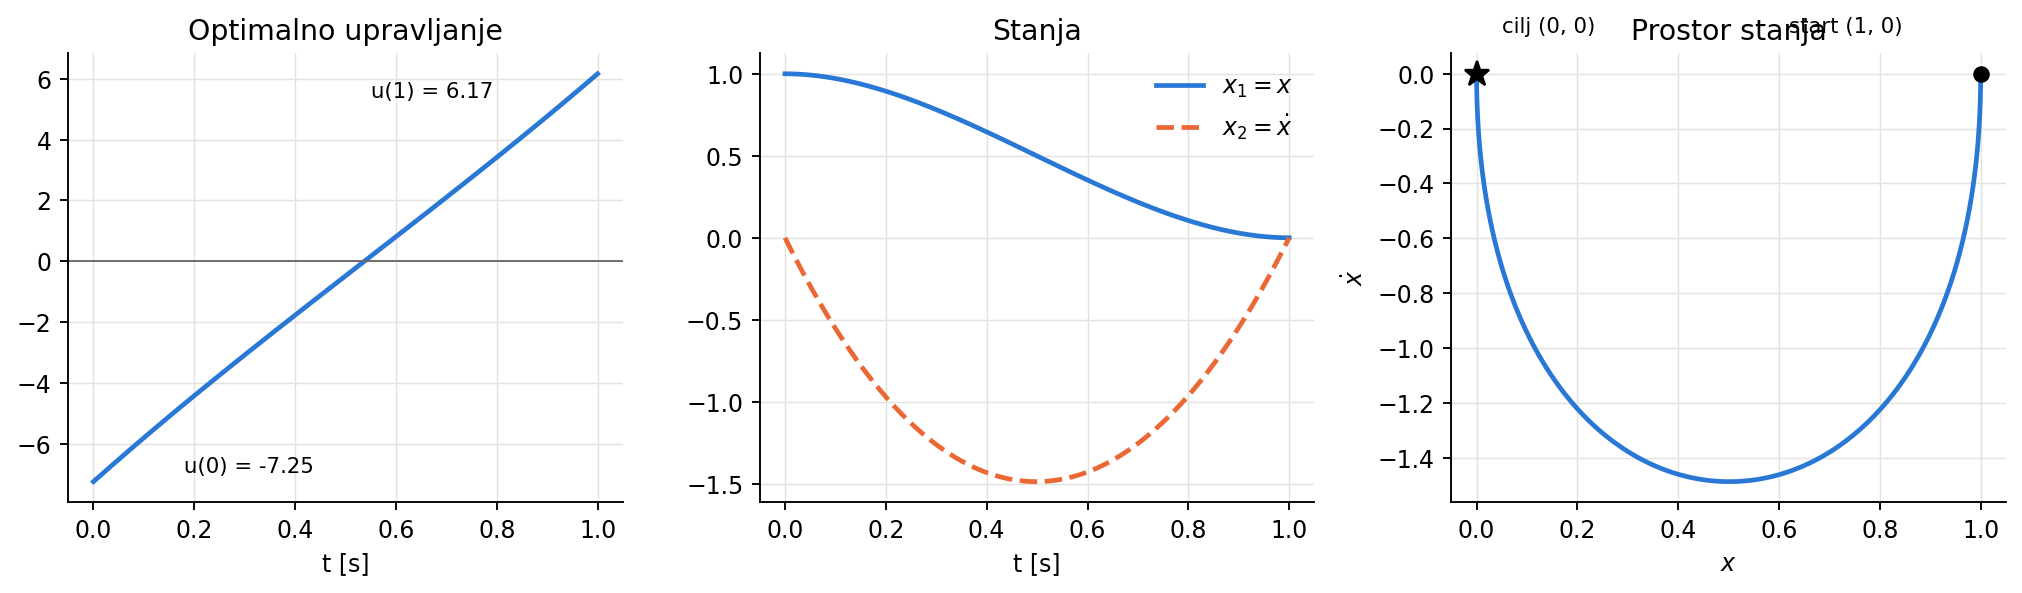
\includegraphics[width=0.95\linewidth,height=\textheight,keepaspectratio,alt={Optimalno rešenje sa zadatim krajem. Levo: u* raste skoro linearno od −7,25 do +6,17. Sredina: x pada od 1 do 0, a brzina ima minimum oko −1,49 na polovini intervala. Desno: putanja u prostoru stanja od (1, 0) do (0, 0).}]{figures/q6_resenje.png}
\caption{Optimalno rešenje sa zadatim krajem. Levo: u* raste skoro linearno od −7,25 do +6,17. Sredina: x pada od 1 do 0, a brzina ima minimum oko −1,49 na polovini intervala. Desno: putanja u prostoru stanja od (1, 0) do (0, 0).}
\end{figure}

\begin{figure}
\centering
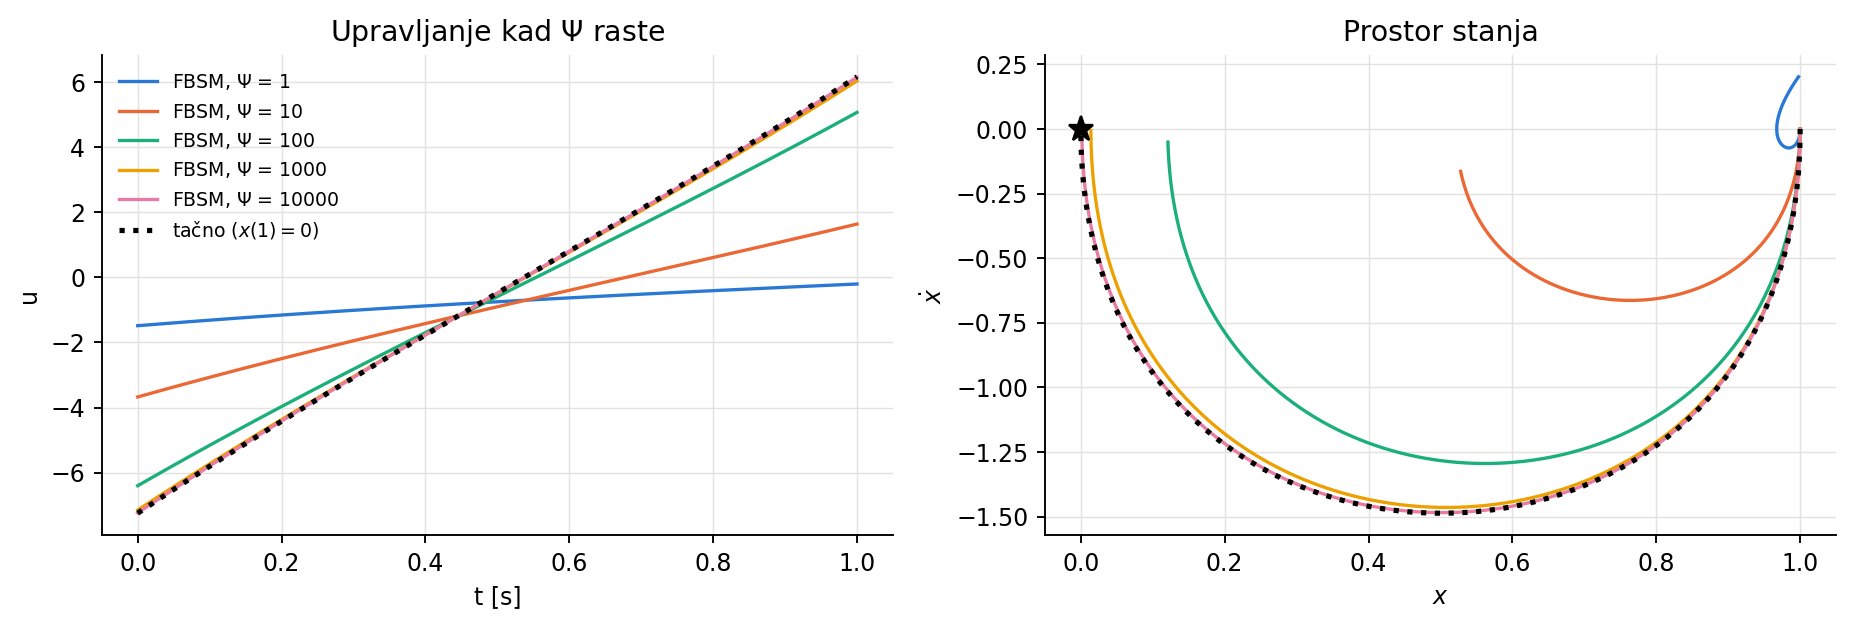
\includegraphics[width=0.95\linewidth,height=\textheight,keepaspectratio,alt={FBSM sa kaznom. Kako Ψ raste, upravljanje i putanja se približavaju tačnom rešenju (tačkasto). Za Ψ = 1 kraj je daleko od nule, a za Ψ = 10⁴ razlika se više ne vidi.}]{figures/q6_fbsm_kazna.png}
\caption{FBSM sa kaznom. Kako Ψ raste, upravljanje i putanja se približavaju tačnom rešenju (tačkasto). Za Ψ = 1 kraj je daleko od nule, a za Ψ = 10⁴ razlika se više ne vidi.}
\end{figure}

\subsection{Tumačenje rezultata}

\begin{itemize}
\item Na početku je \(u < 0\) i veliko: nestabilni mod \(e^t\) bi odvukao \(x\) naviše, pa ga upravljanje odmah „vuče'' nadole.
\item Oko \(t = 0{,}5\) upravljanje menja znak, a posle toga koči, da bi sistem stao u nuli (\(\dot x(1) = 0\)).
\item \(u^*(t)\) nije relejno, jer je \(H\) kvadratan po \(u\). Poređenje: u pitanjima 7 i 8 je \(H\) linearan po \(u\) i rešenje je \(\pm1\).
\end{itemize}

\begin{ispit}[{Pitanje 6}]
\begin{itemize}
\item Odmah reći: tekst zadaje samo \(x(0) = 1\); sa slobodnim krajem rešenje je \(u \equiv 0\). Usvaja se \((1, 0) \to (0, 0)\).
\item Oslonac za izbor: profesor je domaći proveravao kao rešen „analitički i numerički, kao \textbf{dvotačkasti granični problem}„, a za izbor je rekao da je „potpuno proizvoljan'' \izvor{P11 snimak, 1. min; P14 snimak, 71. min}. Pravi dvotačkasti problem postoji tek sa uslovima na oba kraja. Konkretan krajnji uslov na snimcima nije izgovoren, pa izbor treba obrazložiti.
\item Napisati \(H\), \(u^* = -p_2/2\), adjungovane jednačine i dvotačkasti problem. Objasniti zašto je težak (\(x\) zadato na krajevima, \(p\) nigde).
\item Opisati FBSM korak po korak i trik sa kaznom \(p(1) = 2\Psi x(1)\) i prigušenjem \(w\).
\item Rezultat: \(I_{min} \approx 14{,}76\), \(u\) od \(-7{,}25\) do \(6{,}17\).
\end{itemize}
\end{ispit}

\subsection{Moguća potpitanja}

\begin{itemize}
\item \textbf{Zašto je sa slobodnim krajem \(u \equiv 0\)?} \(\dot p_1 = -p_2\), \(\dot p_2 = -p_1\) ne zavise od \(x\), pa uz \(p(1) = 0\) daju \(p \equiv 0\), tj. \(u = -p_2/2 \equiv 0\). Kriterijum ne kažnjava stanje, pa je najjeftinije ne raditi ništa.
\item \textbf{Zašto upravljanje nije relejno?} \(H\) je kvadratan po \(u\) (\(\partial^2H/\partial u^2 = 2 > 0\)), pa je minimum unutrašnja tačka \(u = -p_2/2\), a ne granica.
\item \textbf{Zašto FBSM ne radi direktno sa \(x(1) = 0\)?} Propagacija unazad kreće od poznatog \(p(T)\), a kod zadatog kraja \(p(1)\) nije poznato. Zato se kraj zamenjuje kaznom \(\Psi\|x(1)\|^2\), pa je \(p(1) = 2\Psi x(1)\).
\item \textbf{Zašto \(w\) mora ići ka 1 kad \(\Psi\) raste?} Tada mala promena \(x(1)\) daje veliku promenu \(p(1)\) i \(u\); bez jakog prigušenja iteracija osciluje i divergira.
\item \textbf{Kako radi gađanje?} Pogodi se \(p(0)\), integrali se sistem od 4 jednačine unapred i meri promašaj \(x(1)\); \(p(0)\) se popravlja (Njutn). Za linearan sistem promašaj je linearan po \(p(0)\).
\item \textbf{Kada zadatak sa zadatim krajem uopšte ima rešenje?} Kad je sistem upravljiv (Gramijan \(W\) je regularan); tada je \(I_{min} = (e^{AT}x_0)^TW^{-1}(e^{AT}x_0)\).
\end{itemize}

\section{7. Ograničeno upravljanje, minimizacija ∫x dt (T = 1 s i T = 2 s)}

Zvaničan tekst: \emph{Izračunati optimalnu strategiju upravljanja i kretanje u prostoru stanja koja kriterijumu optimalnosti \(I = \int_0^T x(t)\,dt\) saopštava minimalnu vrednost. Proces je opisan sa \(\dot x = u\), uz početne uslove \(x(0) = 1\). Upravljanje je ograničeno vrednostima \(-1 \le u(t) \le 1\). Problem rešiti za \(T = 1\) s i \(T = 2\) s.} \izvor{zadatak 7}

\begin{kljucna}[{Odgovor u 60 sekundi}]
\begin{enumerate}
\def\labelenumi{\arabic{enumi}.}
\item \(H = x + p\,u\) je \textbf{linearan} po \(u\), a \(u\) je ograničeno, pa se \(\partial H/\partial u = 0\) ne može koristiti (\(\partial H/\partial u = p\) ne zavisi od \(u\)).
\item Princip minimuma: \(u^*\) minimizuje \(H\) po \(u \in [-1, 1]\), pa je \(u^* = -\operatorname{sign} p\) (relejno upravljanje).
\item \(\dot p = -\partial H/\partial x = -1\), a \(x(T)\) je slobodno, pa \(p(T) = 0\). Zato je \(p(t) = T - t \ge 0\).
\item \(p\) ne menja znak, pa nema prekidanja: \(u^* = -1\) na celom intervalu, \(x^*(t) = 1 - t\).
\item \(I_{min} = T - T^2/2\): za \(T = 1\) je \(I = 0{,}5\) (\(x(1) = 0\)), a za \(T = 2\) je \(I = 0\) (\(x(2) = -1\)).
\item Provera zdravim razumom: \(\dot x \ge -1\), pa je \(x(t) \ge 1 - t\) u svakom trenutku; \(u = -1\) je najbolje u svakom trenutku.
\end{enumerate}
\end{kljucna}

\subsection{Ideja}

Želimo da površina ispod \(x(t)\) bude što manja, a \(x\) možemo da menjamo najviše brzinom 1. Intuitivno: treba spuštati \(x\) što brže, sve vreme. Zadatak služi da se pokaže \textbf{mehanizam} principa minimuma kod ograničenog upravljanja: kad je \(H\) linearan po \(u\), optimum je na granici, a o granici odlučuje znak koeficijenta uz \(u\).

\subsection{Rešenje}

\textbf{Hamiltonijan.} \(F = x\), \(f = u\):

\[H = x + p\,u .\]

\textbf{Zašto ne \(\partial H/\partial u = 0\).} \(\partial H/\partial u = p\). Uslov bi dao \(p \equiv 0\), a onda bi \(\dot p = -1\) bilo nemoguće. Znači, minimum \(H\) po \(u\) nije u unutrašnjosti intervala, nego na granici.

\textbf{Princip minimuma.} U \(H\) od \(u\) zavisi samo član \(p\,u\). Da bi bio što manji:

\[u^* = \begin{cases} -1, & p > 0 \\ +1, & p < 0 \end{cases} \qquad\text{tj.}\qquad u^* = -\operatorname{sign} p .\]

To je \textbf{relejno} (bang-bang) upravljanje: dvopoložajni regulator.

\textbf{Adjungovana promenljiva.}

\[\dot p = -\frac{\partial H}{\partial x} = -1, \qquad x(T) \text{ slobodno} \;\Rightarrow\; p(T) = 0 \;\Rightarrow\; p(t) = T - t .\]

Za \(0 \le t < T\) je \(p > 0\). Pošto je \(p\) monotona funkcija koja dostiže nulu tek u \(t = T\), \textbf{nema prekidanja}:

\[u^*(t) = -1 \quad\text{na celom } [0, T] .\]

\textbf{Kretanje.} \(\dot x = -1\), \(x(0) = 1\):

\[x^*(t) = 1 - t, \qquad I_{min} = \int_0^T(1 - t)\,dt = T - \frac{T^2}{2} .\]

\textbf{Provera \(H = \text{const}\).} \(H = x + p\,u = (1 - t) + (T - t)(-1) = 1 - T\), konstantno. Pošto je \(T\) zadato, ne mora biti nula.

\subsubsection{a) T = 1 s}

\[u^* = -1, \qquad x^*(t) = 1 - t, \qquad p(t) = 1 - t, \qquad x(1) = 0, \qquad I_{min} = 0{,}5 .\]

\subsubsection{b) T = 2 s}

\[u^* = -1, \qquad x^*(t) = 1 - t, \qquad p(t) = 2 - t, \qquad x(2) = -1, \qquad I_{min} = 0 .\]

Za \(t > 1\) je \(x < 0\), i to je optimalno: negativno \(x\) smanjuje integral, pa se pozitivna površina do \(t = 1\) poništi negativnom posle \(t = 1\). U zadatku nema ograničenja \(x \ge 0\). (Da ga ima, optimalno bi bilo \(u = -1\) do \(t = 1\), pa \(u = 0\), i \(I = 0{,}5\). To je provereno numerički samo radi poređenja.)

\begin{figure}
\centering
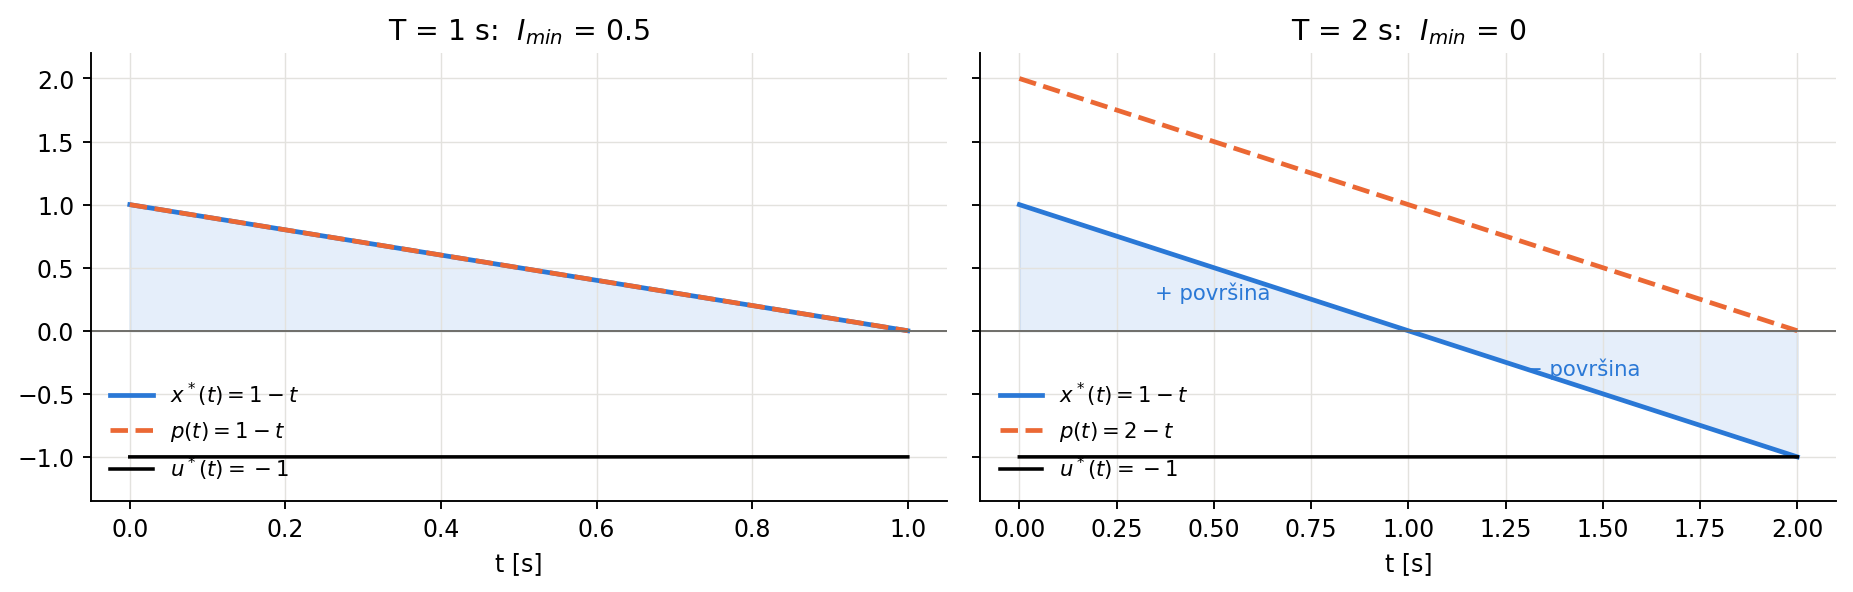
\includegraphics[width=0.9\linewidth,height=\textheight,keepaspectratio,alt={Rešenje zadatka 7 za T = 1 i T = 2. Upravljanje je −1 sve vreme, jer p(t) = T − t ne menja znak. Za T = 2 stanje prelazi u negativno, pa površina posle t = 1 poništava površinu pre t = 1 i I = 0.}]{figures/q7_T1_T2.png}
\caption{Rešenje zadatka 7 za T = 1 i T = 2. Upravljanje je −1 sve vreme, jer p(t) = T − t ne menja znak. Za T = 2 stanje prelazi u negativno, pa površina posle t = 1 poništava površinu pre t = 1 i I = 0.}
\end{figure}

\subsection{Intuitivna provera (dokaz bez principa minimuma)}

Za svako dozvoljeno upravljanje je \(\dot x = u \ge -1\), pa integracijom od 0:

\[x(t) = 1 + \int_0^t u\,d\tau \ge 1 - t \qquad\text{za svako } t .\]

Znači da nijedno dozvoljeno upravljanje ne može dati manje \(x(t)\) ni u jednom trenutku nego \(u = -1\). Pošto je \(I\) integral od \(x\), \(u = -1\) je optimalno. Ovo je jak argument za usmeni ispit: pokazuje da rezultat ima smisla i bez računa.

\subsection{Numerička provera}

\begin{longtable}[]{@{}
  >{\raggedright\arraybackslash}p{(\linewidth - 6\tabcolsep) * \real{0.2105}}
  >{\centering\arraybackslash}p{(\linewidth - 6\tabcolsep) * \real{0.2632}}
  >{\centering\arraybackslash}p{(\linewidth - 6\tabcolsep) * \real{0.2632}}
  >{\centering\arraybackslash}p{(\linewidth - 6\tabcolsep) * \real{0.2632}}@{}}
\caption{Tri nezavisna rešenja}\tabularnewline
\toprule\noalign{}
\begin{minipage}[b]{\linewidth}\raggedright
\end{minipage} & \begin{minipage}[b]{\linewidth}\centering
analitički
\end{minipage} & \begin{minipage}[b]{\linewidth}\centering
FBSM (\(u = -\operatorname{sign}p\))
\end{minipage} & \begin{minipage}[b]{\linewidth}\centering
linearno programiranje
\end{minipage} \\
\midrule\noalign{}
\endfirsthead
\toprule\noalign{}
\begin{minipage}[b]{\linewidth}\raggedright
\end{minipage} & \begin{minipage}[b]{\linewidth}\centering
analitički
\end{minipage} & \begin{minipage}[b]{\linewidth}\centering
FBSM (\(u = -\operatorname{sign}p\))
\end{minipage} & \begin{minipage}[b]{\linewidth}\centering
linearno programiranje
\end{minipage} \\
\midrule\noalign{}
\endhead
\bottomrule\noalign{}
\endlastfoot
\(T = 1\) & 0,5 & 0,5 (2 iteracije) & 0,5; \(u = -1\) na 100\% intervala \\
\(T = 2\) & 0 & 0 (2 iteracije) & 0; \(u = -1\) na 100\% intervala \\
\end{longtable}

Linearno programiranje ne pretpostavlja oblik upravljanja (samo diskretizuje \(u\) na 400 delova sa \(|u| \le 1\)), pa potvrđuje da relejno rešenje nije posledica pretpostavke. FBSM konvergira u dve iteracije jer \(p(t)\) ne zavisi od \(x\).

\subsection{Opšte pravilo za relejno upravljanje}

Ovde je \(h = p\) (koeficijent uz \(u\) u \(H = H_0 + h\,u\)). Opšte pravilo (\(u^* = u_{min}\) za \(h > 0\), \(u_{max}\) za \(h < 0\); broj prekidanja = broj promena znaka \(h\); „tri pomoći'' za izbor strategije) je u odeljku „Zajednički alat''.

\begin{ispit}[{Pitanje 7}]
\begin{itemize}
\item Glavna poruka: \(H\) linearan po \(u\) + ograničeno \(u\) → relejno upravljanje; \(\partial H/\partial u = 0\) ne važi.
\item Obavezno: \(p(T) = 0\) jer je \(x(T)\) slobodno; \(p = T - t \ge 0\), pa nema prekidanja.
\item Za \(T = 2\) objasniti zašto je \(x < 0\) dozvoljeno i daje \(I = 0\).
\item Zamka: pomisliti da za \(T = 2\) treba stati u nuli (\(u = 0\) posle \(t = 1\)). To bi bilo tačno samo uz ograničenje \(x \ge 0\).
\end{itemize}
\end{ispit}

\subsection{Moguća potpitanja}

\begin{itemize}
\item \textbf{Zašto je \(p(T) = 0\)?} \(x(T)\) nije zadato (slobodan kraj), a kriterijum nema član \(\Psi\) (pitanje 1).
\item \textbf{Šta je sa \(u\) u trenutku \(t = T\), gde je \(p = 0\)?} To je jedna tačka, pa vrednost \(u\) tu ne utiče na \(x\) ni na \(I\).
\item \textbf{Može li postojati singularno upravljanje (\(p \equiv 0\) na nekom intervalu)?} Ne: \(\dot p = -1 \ne 0\), pa \(p\) ne može biti nula na intervalu. Uopšte, na pitanje da li upravljanje može delom biti glatko profesor kaže „teoretski da, praktično ne'' \izvor{P11 snimak, 83. min}.
\item \textbf{Šta ako je kraj zadat, npr. \(x(2) = 0\)?} Tada \(p(2)\) nije poznato, \(p = c - t\) menja znak jednom: \(u = -1\) do \(t_1\), pa \(u = +1\). Iz \(x(2) = 1 - t_1 + (2 - t_1) = 0\) sledi \(t_1 = 1{,}5\) (spusti se do \(-0{,}5\), pa se vrati).
\item \textbf{Šta ako se kriterijum maksimizuje?} Znak se obrće: \(u^* = +\operatorname{sign} p\) (tj. \(u = +1\)), \(x = 1 + t\).
\item \textbf{Zašto \(H\) nije nula?} \(T\) je zadato, pa važi samo \(H = \text{const}\) (autonoman sistem), ovde \(H = 1 - T\); \(H = 0\) važi samo za slobodno \(T\).
\end{itemize}

\section{8. Analitičko rešenje: problem minimuma vremena (dvostruki integrator)}

Zvaničan tekst: \emph{Analitički rešiti optimizacioni problem \(\dot x_1 = x_2\), \(\dot x_2 = u\), \(x_1(0) = 2\), \(x_2(0) = -1\), \(x_1(T) = 0\), \(x_2(T) = 0\), pri čemu je kriterijum optimalnosti \(I = \int_0^T dt\). Upravljanje je ograničeno vrednostima \(-1 \le u(t) \le 1\).} \izvor{zadatak 8}

\begin{kljucna}[{Odgovor u 60 sekundi}]
\begin{enumerate}
\def\labelenumi{\arabic{enumi}.}
\item Minimum vremena: \(F = 1\), \(H = 1 + p_1x_2 + p_2u\). \(H\) je linearan po \(u\), pa je \(u^* = -\operatorname{sign}p_2 = \pm1\).
\item \(\dot p_1 = 0\), \(\dot p_2 = -p_1\), pa je \(p_2 = c_2 - c_1t\) linearno i menja znak \textbf{najviše jednom}: najviše jedno prekidanje.
\item Za \(u = \pm1\) fazne trajektorije su parabole \(x_1 = \pm\frac12x_2^2 + A\). U nulu se stiže samo po dve parabole kroz koordinatni početak: to je kriva prekidanja \(x_1 = -\frac12x_2|x_2|\).
\item Tačka \((2, -1)\) je iznad krive, pa se ide prvo \(u = -1\), do preseka sa granom \(x_1 = \frac12x_2^2\), pa \(u = +1\) do nule.
\item Presek je \((1{,}25;\ -1{,}581)\), prekidanje u \(t_1 = \sqrt{2{,}5} - 1 = 0{,}581\) s, a \(T_{min} = 2\sqrt{2{,}5} - 1 = 2{,}162\) s.
\item \(T\) je nepoznato, pa je \(H \equiv 0\); iz toga je \(c_1 = 1/\sqrt{2{,}5}\) i \(p_2 = 0{,}632\,(0{,}581 - t)\), što potvrđuje redosled \(-1 \to +1\).
\end{enumerate}
\end{kljucna}

\subsection{Ideja}

Dvostruki integrator je model tela koje se pomera silom \(u\) bez trenja: \(x_1\) je položaj, \(x_2\) brzina. Treba ga što brže dovesti u mirovanje u nuli, sa ograničenom silom. Intuicija je ista kao kod vožnje: punim gasom ka cilju, pa punom kočnicom, tačno u pravom trenutku. Princip minimuma to potvrđuje i daje trenutak prebacivanja.

Profesor ovako uvodi zadatak: sistem je izveden iz ravnotežnog stanja u tačku \((\alpha, \beta)\) i treba ga u najkraćem vremenu vratiti u ravnotežu. Minimum vremena je „prvi kriterijum koji smo napisali na optimizaciji'', a tek sada, posle dve godine, može da se reši, jer je upravljanje ograničeno \izvor{P12 snimak, 1.--3. min}.

\subsection{Postavka}

\[\dot x_1 = x_2, \qquad \dot x_2 = u, \qquad x(0) = (2, -1), \qquad x(T) = (0, 0), \qquad |u| \le 1, \qquad I = \int_0^T dt = T \to \min .\]

Opšti postupak je obrađen na predavanju za proizvoljan početak \((\alpha, \beta)\). Profesor ističe da za minimum vremena „ne postoji opšte rešenje, tj. teorija, samo opšti princip rešavanja''.

\subsection{Rešenje}

\textbf{Korak 1: Hamiltonijan i upravljanje.}

\[H = 1 + p_1x_2 + p_2u .\]

Od \(u\) zavisi samo \(p_2u\) (profesor ga zove \(H^*\)). Minimizacija po \(u \in [-1, 1]\):

\[u^* = \begin{cases} -1, & p_2 > 0 \\ +1, & p_2 < 0 \end{cases} \qquad\text{tj.}\qquad u^* = -\operatorname{sign}p_2 .\]

\(p_2\) i \(u\) moraju biti suprotnog znaka.

\textbf{Korak 2: adjungovane jednačine.}

\[\dot p_1 = -\frac{\partial H}{\partial x_1} = 0 \;\Rightarrow\; p_1 = c_1, \qquad \dot p_2 = -\frac{\partial H}{\partial x_2} = -p_1 \;\Rightarrow\; p_2 = c_2 - c_1t .\]

\(p_2\) je \textbf{linearna} funkcija vremena, pa menja znak najviše jednom. Moguća su samo četiri niza upravljanja: \(+1\); \(-1\); \(+1 \to -1\); \(-1 \to +1\) {[}četiri skice znaka \(c_1; c_2\){]}.

\textbf{Korak 3: trajektorije u faznoj ravni.} Eliminiše se vreme: \(\frac{dx_1}{dx_2} = \frac{x_2}{u}\).

\begin{itemize}
\item \(u = +1\): \(x_2 = t + A\), \(x_1 = \frac{t^2}{2} + At + B = \frac12(t + A)^2 + \big(B - \frac12A^2\big)\), pa je \(x_1 = \frac12x_2^2 + A_1\).
\item \(u = -1\): \(x_2 = -t + C\), \(x_1 = -\frac{t^2}{2} + Ct + D = -\frac12(-t + C)^2 + \big(D + \frac12C^2\big)\), pa je \(x_1 = -\frac12x_2^2 + A_2\).
\end{itemize}

(Dopuna do punog kvadrata: dodaje se i oduzima \(\frac12A^2\).) Na predavanju se familija za \(u = +1\) označava sa \(\Gamma^+\), a za \(u = -1\) sa \(\Gamma^-\) \izvor{P12 snimak, 25.--27. min}.

\textbf{Korak 4: kriva prekidanja.} U \((0, 0)\) se može ući samo po paraboli koja kroz nju prolazi:

\begin{itemize}
\item sa \(u = +1\) po \(x_1 = \frac12x_2^2\), i to po grani \(x_2 < 0\) (brzina raste ka nuli),
\item sa \(u = -1\) po \(x_1 = -\frac12x_2^2\), po grani \(x_2 > 0\) (brzina opada ka nuli).
\end{itemize}

Unija te dve grane je \textbf{kriva prekidanja}:

\[x_1 = -\frac12\,x_2|x_2| .\]

Iznad (desno od) krive je \(u = -1\), a ispod (levo) je \(u = +1\). Posle jednog prekidanja stanje mora biti na krivoj, jer se drugačije ne može stići u nulu bez novog prekidanja.

\textbf{Korak 5: gde je početna tačka?} Za \(x_2 = -1\) kriva daje \(x_1 = -\frac12(-1)\cdot1 = 0{,}5\). Početno \(x_1 = 2 > 0{,}5\), pa je tačka \textbf{iznad} krive. Kreće se sa \(u = -1\), a na \(u = +1\) prelazi se na grani \(x_1 = \frac12x_2^2\), \(x_2 < 0\).

\textbf{Korak 6: prvi luk (\(u = -1\)).} Parabola kroz \((2, -1)\):

\[2 = -\frac12(-1)^2 + A_2 \;\Rightarrow\; A_2 = 2{,}5, \qquad x_1 = -\frac12x_2^2 + 2{,}5 .\]

U vremenu: \(x_2(t) = -1 - t\), \(x_1(t) = 2 - t - \frac12t^2\).

\textbf{Korak 7: tačka prekidanja} (presek sa \(x_1 = \frac12x_2^2\)):

\[\frac12x_2^2 = -\frac12x_2^2 + 2{,}5 \;\Rightarrow\; x_2^2 = 2{,}5 \;\Rightarrow\; x_2 = -\sqrt{2{,}5} = -1{,}5811, \qquad x_1 = 1{,}25 .\]

Negativan koren, jer je grana \(u = +1\) na \(x_2 < 0\). Ova tačka se na predavanju zove \textbf{tačka priključenja} \(C\). Vreme prekidanja se čita iz \(x_2\), jer se \(x_2\) menja brzinom 1:

\[-1 - t_1 = -\sqrt{2{,}5} \;\Rightarrow\; t_1 = \sqrt{2{,}5} - 1 = 0{,}5811 \text{ s} .\]

\textbf{Korak 8: drugi luk (\(u = +1\)).} \(x_2\) raste brzinom 1 od \(-\sqrt{2{,}5}\) do 0, što traje \(\sqrt{2{,}5}\) s:

\begin{kljucna}
\[T_{min} = t_1 + \sqrt{2{,}5} = 2\sqrt{2{,}5} - 1 \approx 2{,}1623 \text{ s}, \qquad u^*(t) = \begin{cases} -1, & 0 \le t < 0{,}5811 \\ +1, & 0{,}5811 \le t \le 2{,}1623 \end{cases}\]
\end{kljucna}

\textbf{Provera opštom formulom sa predavanja.} Za tačku \((\alpha, \beta)\) iznad krive izvedeno je \(t_p = \beta + \sqrt{\alpha + \frac12\beta^2}\) i \(T = \beta + 2\sqrt{\alpha + \frac12\beta^2}\). Za \(\alpha = 2\), \(\beta = -1\): \(\sqrt{2 + 0{,}5} = \sqrt{2{,}5}\), pa je \(t_p = 0{,}581\) i \(T = 2{,}162\), isto.

\textbf{Korak 9: konstante \(p\) i provera preko \(H \equiv 0\).} U trenutku prekidanja je \(p_2(t_1) = 0\), pa je \(c_2 = c_1t_1\). \(T\) nije zadato (pitanje 2), a sistem je autonoman, pa je \(H \equiv 0\). U \(t = 0\) (\(x_2 = -1\), \(u = -1\)):

\[1 + c_1\cdot(-1) + c_1t_1\cdot(-1) = 0 \;\Rightarrow\; c_1 = \frac{1}{1 + t_1} = \frac{1}{\sqrt{2{,}5}} = 0{,}6325 .\]

\[p_1 = 0{,}6325, \qquad p_2(t) = 0{,}6325\,(0{,}5811 - t) .\]

\(p_2 > 0\) pre \(t_1\) (daje \(u = -1\)) i \(p_2 < 0\) posle (daje \(u = +1\)). Rešenje je konzistentno sa principom minimuma.

\begin{figure}
\centering
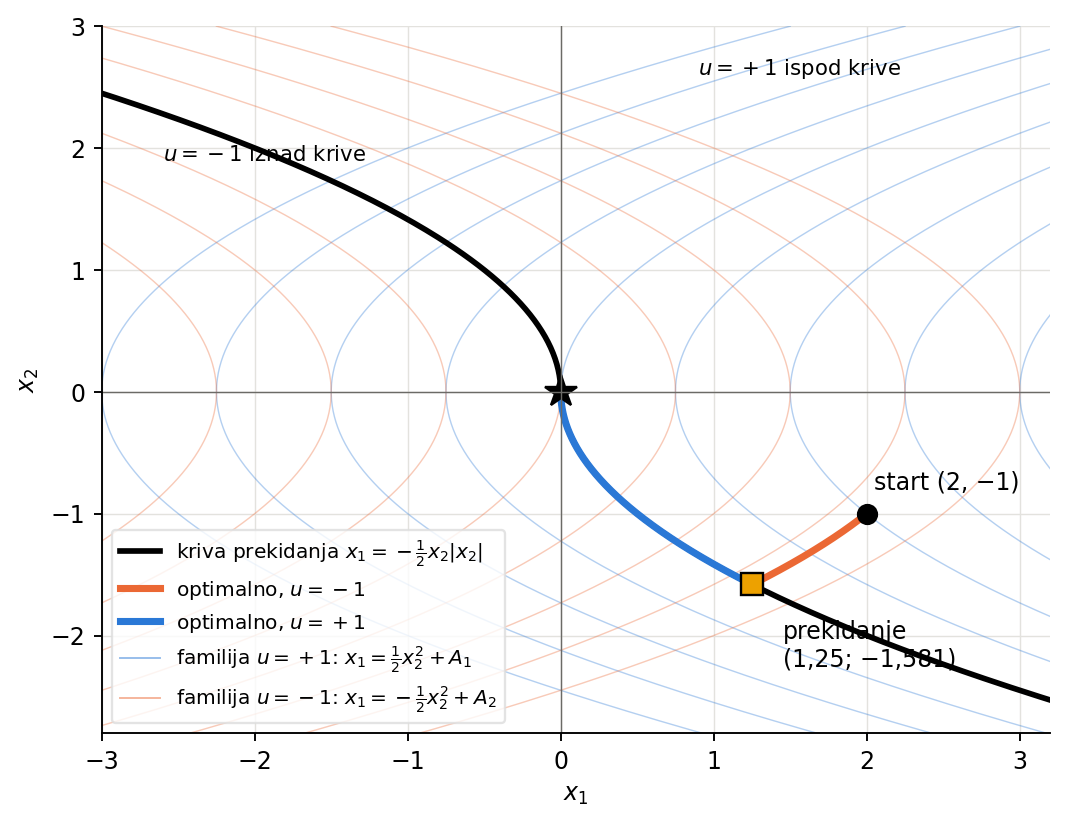
\includegraphics[width=0.8\linewidth,height=\textheight,keepaspectratio,alt={Fazna ravan za zadatak 8. Tanke linije su familije parabola za u = +1 i u = −1. Crna kriva je kriva prekidanja. Iz (2, −1) se ide sa u = −1 (narandžasto) do preseka (1,25; −1,581), pa sa u = +1 (plavo) po krivoj prekidanja u nulu.}]{figures/q8_fazna_ravan.png}
\caption{Fazna ravan za zadatak 8. Tanke linije su familije parabola za u = +1 i u = −1. Crna kriva je kriva prekidanja. Iz (2, −1) se ide sa u = −1 (narandžasto) do preseka (1,25; −1,581), pa sa u = +1 (plavo) po krivoj prekidanja u nulu.}
\end{figure}

\begin{figure}
\centering
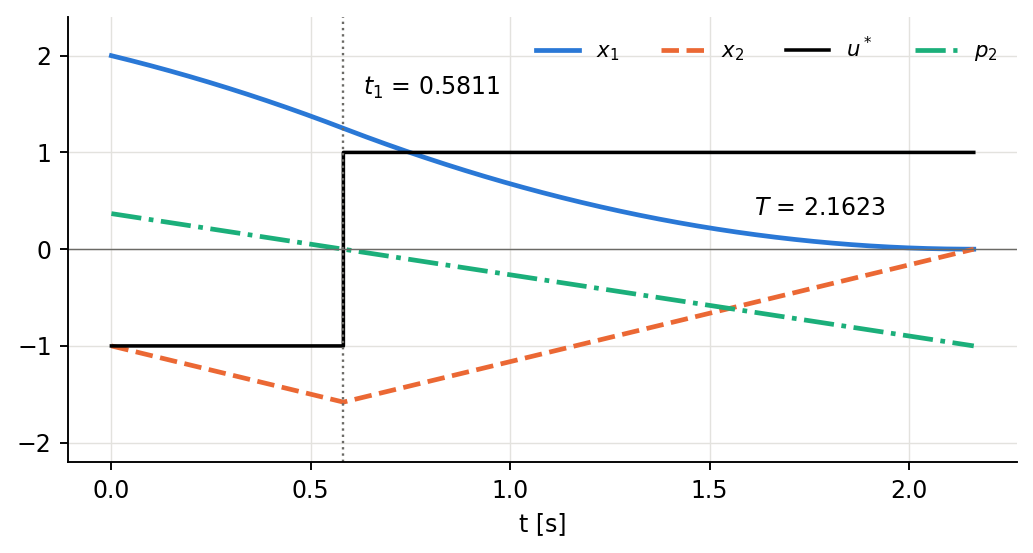
\includegraphics[width=0.8\linewidth,height=\textheight,keepaspectratio,alt={Isto rešenje u vremenu. Upravljanje skače sa −1 na +1 tačno kada p₂ prolazi kroz nulu. Brzina x₂ je izlomljena prava, a položaj x₁ glatko ulazi u nulu u T = 2,162 s.}]{figures/q8_vreme.png}
\caption{Isto rešenje u vremenu. Upravljanje skače sa −1 na +1 tačno kada p₂ prolazi kroz nulu. Brzina x₂ je izlomljena prava, a položaj x₁ glatko ulazi u nulu u T = 2,162 s.}
\end{figure}

\subsection{Numerička provera}

\begin{itemize}
\item Simulacija sa ovim \(u^*\) završava tačno u \((0, 0)\), a \(\max|H| = 2\cdot10^{-16}\) duž putanje.
\item Nezavisno: za zadato \(T\) pitanje „postoji li \(|u| \le 1\) koje dovodi sistem u nulu'' je problem linearnog programiranja. Bisekcijom po \(T\) dobija se najmanje izvodljivo \(T_{min} = 2{,}1623\) s. Ova provera ne koristi ni princip minimuma ni krivu prekidanja.
\end{itemize}

\begin{ispit}[{Pitanje 8}]
\begin{itemize}
\item Redosled: \(H\) → \(u = -\operatorname{sign}p_2\) → \(p_2\) linearno → najviše jedno prekidanje → parabole → kriva prekidanja → položaj početne tačke → presek → vremena.
\item Obavezno nacrtati faznu ravan sa krivom prekidanja i putanjom.
\item Zamke: pogrešan znak korena (\(x_2 = +\sqrt{2{,}5}\)), pogrešan redosled (\(+1 \to -1\)), računanje \(t_1\) iz \(x_1\) umesto iz \(x_2\).
\item Završiti sa \(H \equiv 0\) (nespecificiran \(T\)) i proverom znaka \(p_2\).
\item Profesor je na času nudio „50\% mog ispita'' onome ko za opšte \((\alpha, \beta)\) izračuna \(t_p\) i \(T\) \izvor{P12 snimak, 33. min}. Znati izvesti \(t_p = \beta + \sqrt{\alpha + \beta^2/2}\) i \(T = \beta + 2\sqrt{\alpha + \beta^2/2}\).
\item Domaći: za različite početne \((\alpha, \beta)\) simulirati familije krivih i znati rešiti svaki slučaj \izvor{P14 snimak, 72. min}.
\end{itemize}
\end{ispit}

\subsection{Moguća potpitanja}

\begin{itemize}
\item \textbf{Zašto najviše jedno prekidanje?} \(p_2 = c_2 - c_1t\) je prava, a prava menja znak najviše jednom.
\item \textbf{Sme li \(c_1 = 0\)?} Sme (pitanje sa predavanja): tada je \(p_2 = c_2\) konstantno, pa je upravljanje isto ceo interval, bez prekidanja \izvor{P12 snimak, 16. min}. Takav kandidat odgovara početnoj tački na krivoj prekidanja.
\item \textbf{Može li \(p_2 \equiv 0\) (singularni slučaj)?} Ne: tada je \(c_1 = c_2 = 0\), pa je \(H = 1 \ne 0\), suprotno uslovu \(H \equiv 0\).
\item \textbf{Zašto je iznad krive \(u = -1\)?} Tu je sistem „previše desno'' za svoju brzinu; ni sa punim \(u = +1\) ne bi stao u nuli, pa prvo mora da ubrza ulevo (\(u = -1\)) dok ne stigne na granu \(x_1 = \frac12x_2^2\).
\item \textbf{Šta ako je početna tačka na krivoj prekidanja?} Nema prekidanja: odmah se ide po krivoj sa jednim \(u\) do nule.
\item \textbf{Da li je ovo upravljanje u zatvorenoj sprezi?} Može se tako napisati: \(u = -\operatorname{sign}\big(x_1 + \frac12x_2|x_2|\big)\) (na samoj krivoj \(u = -\operatorname{sign}x_2\)). Ovde je to izuzetak koji daje geometrija fazne ravni, ne sam Pontrjagin.
\item \textbf{Šta ako je \(|u| \le U\)?} Parabole su \(x_1 = \pm\frac{x_2^2}{2U} + A\), kriva prekidanja \(x_1 = -\frac{x_2|x_2|}{2U}\), a postupak je isti.
\end{itemize}

\section{9. Hamilton--Jakobi--Belmanova jednačina: izvođenje}

\begin{kljucna}[{Odgovor u 60 sekundi}]
\begin{enumerate}
\def\labelenumi{\arabic{enumi}.}
\item Belmanov princip optimalnosti: svaki deo optimalnog procesa je i sam optimalan. Ako je put \(A \to B\) optimalan i prolazi kroz \(C\), onda je i deo \(C \to B\) optimalan.
\item Definiše se funkcija optimalne vrednosti \(S(t_0, x_0) = \min_u\int_{t_0}^{t_1}F\,dt\): najmanja cena od stanja \(x_0\) u trenutku \(t_0\) do kraja.
\item Iz principa: \(S(t_0, x_0) = \min_u\big\{\int_{t_0}^{\tau}F\,dt + S[\tau, x^*(\tau)]\big\}\), za \(\tau = t_0 + dt\).
\item Prvi deo je \(F\,dt\), a \(S[\tau, x^*(\tau)]\) se razvije u Tejlorov red: \(S + \frac{\partial S}{\partial t}dt + \frac{\partial S}{\partial x}f\,dt\).
\item \(S(t_0, x_0)\) se skrati sa obe strane, sve se podeli sa \(dt\): \(\frac{\partial S}{\partial t} + \min_u\big[F + \frac{\partial S}{\partial x}f\big] = 0\).
\item Sa \(p = \partial S/\partial x\) zagrada je Hamiltonijan: \(\frac{\partial S}{\partial t} + H^*\big(t, x, \frac{\partial S}{\partial x}\big) = 0\), uz \(S(t_1, x) = \Psi(x)\).
\item Rešenje je \(u^* = \Theta(t, x)\): upravljanje u zatvorenoj sprezi. Cena je parcijalna diferencijalna jednačina.
\end{enumerate}
\end{kljucna}

\subsection{Ideja}

Pontrjagin traži celu optimalnu putanju odjednom, za jedan zadati početak. Belman umesto toga pita: kolika je najmanja preostala cena \textbf{iz bilo kog stanja \(x\) u bilo kom trenutku \(t\)}? Ta funkcija \(S(t, x)\) sadrži rešenje za sve početne uslove, pa iz nje izlazi upravljanje kao funkcija trenutnog stanja, tj. regulator u povratnoj sprezi. Jednačina za \(S\) se dobija iz jednostavnog zapažanja: ako je ceo put optimalan, onda je optimalan i njegov ostatak.

\subsection{Postavka}

\[\dot x = f(t, x, u), \qquad x(t_0) = x_0, \qquad t_0 \le t \le t_1 \text{ poznato}, \qquad I = \int_{t_0}^{t_1}F(t, x, u)\,dt \;\to\; \min\]

Profesor naglašava da je početna vrednost „jako bitna'': \(S\) je funkcija početnog trenutka i početnog stanja \izvor{OptControl2022 sl. 13--16}.

\subsection{Izvođenje}

\textbf{Korak 1: princip optimalnosti.} „Every part of an optimal process is an optimal as well'' \izvor{OptControl2022 sl. 5}. Ako je putanja \(A \to B\) optimalna i prolazi kroz \(C\), onda je \(\min I_{AB} = I_{AC} + I_{CB}\) i deo \(C \to B\) je takođe optimalan. Dokaz je kontradikcijom: kad bi postojao jeftiniji put od \(C\) do \(B\), zamenio bi se, pa bi ceo put \(A \to B\) bio jeftiniji od optimalnog. (Obrnuto ne važi: optimalan ostatak ne znači optimalan ceo put.) Profesorova slika: ako je autoput najbolji put od Novog Sada do Beograda, onda je i njegov deo od Inđije do Beograda najbolji put od Inđije do Beograda \izvor{P14 snimak, 3. min}.

\begin{figure}
\centering
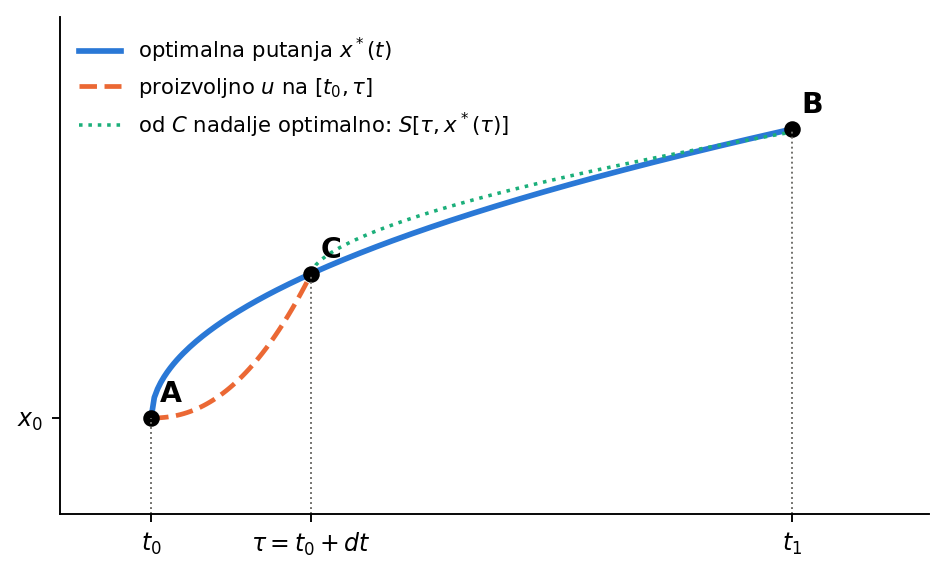
\includegraphics[width=0.7\linewidth,height=\textheight,keepaspectratio,alt={Princip optimalnosti. Put A → C se prelazi proizvoljnim upravljanjem, a od C do B optimalno. Najmanja ukupna cena se dobija kad se i prvi deo izabere optimalno, i tada je to S(t₀, x₀).}]{figures/q9_princip_optimalnosti.png}
\caption{Princip optimalnosti. Put A → C se prelazi proizvoljnim upravljanjem, a od C do B optimalno. Najmanja ukupna cena se dobija kad se i prvi deo izabere optimalno, i tada je to S(t₀, x₀).}
\end{figure}

\textbf{Korak 2: funkcija optimalne vrednosti.}

\[S(t_0, x_0) = \int_{t_0}^{t_1}F\big(t, x_{opt}(t), u_{opt}(t)\big)\,dt = \min_u\int_{t_0}^{t_1}F(t, x, u)\,dt .\]

\textbf{Korak 3: podela intervala.} Za međutrenutak \(\tau\) (\(t_0 \le \tau \le t_1\)), na \([t_0, \tau]\) se bira upravljanje, a od \(\tau\) do kraja se ide optimalno, što košta \(S[\tau, x^*(\tau)]\):

\[S(t_0, x_0) = \min_u\Big\{\int_{t_0}^{\tau}F(t, x, u)\,dt + S\big[\tau, x^*(\tau)\big]\Big\} .\]

Zašto jednakost: najmanja vrednost kriterijuma je jedinstvena. Ako do Skupštine u Beogradu može optimalno da se stigne i preko Gazele i preko Brankovog mosta, oba puta moraju trajati isto; da jedan traje kraće, drugi ne bi bio optimalan \izvor{P14 snimak, 13.--15. min}. Ovaj korak je „čisto logički'', a ostatak izvođenja (razvoj u red) „čisto matematički''.

\textbf{Korak 4: mali korak.} Neka je \(\tau = t_0 + dt\). Za malo \(dt\):

\begin{itemize}
\item stanje se pomeri po jednačini sistema: \(x^*(\tau) = x^*(t_0 + dt) \approx x_0 + \frac{dx}{dt}dt = x_0 + f(t_0, x_0, u_0)\,dt\),
\item integral je površina pravougaonika: \(\int_{t_0}^{t_0 + dt}F\,dt \approx F(t_0, x_0, u_0)\,dt\),
\item \(S\) se razvije u Tejlorov red po oba argumenta:
\end{itemize}

\[S\big[\tau, x^*(\tau)\big] \approx S(t_0, x_0) + \frac{\partial S(t_0, x_0)}{\partial t}dt + \frac{\partial S(t_0, x_0)}{\partial x}f(t_0, x_0, u_0)\,dt .\]

\textbf{Korak 5: zamena.}

\[S(t_0, x_0) = \min_{u_0}\Big\{F(t_0, x_0, u_0)\,dt + S(t_0, x_0) + \frac{\partial S(t_0, x_0)}{\partial t}dt + \frac{\partial S(t_0, x_0)}{\partial x}f(t_0, x_0, u_0)\,dt\Big\} .\]

\(S(t_0, x_0)\) i \(\frac{\partial S}{\partial t}dt\) ne zavise od \(u_0\), pa izlaze ispred \(\min\). \(S(t_0, x_0)\) se skrati sa leve i desne strane, a ostatak se podeli sa \(dt\) i pusti \(dt \to 0\) (greške aproksimacija iz koraka 4 su reda \(dt^2\), pa posle deljenja nestaju):

\[\frac{\partial S(t_0, x_0)}{\partial t} + \min_{u_0}\Big\{F(t_0, x_0, u_0) + \frac{\partial S(t_0, x_0)}{\partial x}f(t_0, x_0, u_0)\Big\} = 0 .\]

\textbf{Korak 6: opšti oblik.} Početni trenutak i stanje su bili proizvoljni, pa se indeks 0 izostavlja („general form without index 0''). Za sistem sa \(n\) stanja \(\frac{\partial S}{\partial x}f\) postaje suma:

\[\frac{\partial S(t, x)}{\partial t} + \min_u\Big\{F(t, x, u) + \sum_{i=1}^n\frac{\partial S}{\partial x_i}f_i(t, x, u)\Big\} = 0 .\]

\textbf{Korak 7: veza sa Hamiltonijanom.} Uvede se

\[p_i = \frac{\partial S(t, x)}{\partial x_i}, \qquad i = 1, \dots, n .\]

Tada je izraz u zagradi upravo \(H = F + \sum p_if_i\) iz Pontrjaginove teorije:

\begin{kljucna}
\textbf{Hamilton--Jakobi--Belmanova jednačina:}

\[\frac{\partial S}{\partial t} + \min_u H\Big(t, x, u, \frac{\partial S}{\partial x}\Big) = 0, \quad\text{tj.}\quad \frac{\partial S}{\partial t} + H^*\Big(t, x, \frac{\partial S}{\partial x}\Big) = 0, \qquad S(t_1, x) = \Psi(x) .\]

\(H^*\) je Hamiltonijan u koji je već uvršteno optimalno \(u\). Jednačina nosi ime Hamiltona zato što sadrži optimalni Hamiltonijan \izvor{P14 snimak, 42. min}; ona je osnova dinamičkog programiranja.
\end{kljucna}

\textbf{Korak 8: postupak rešavanja} \izvor{OptControl2022 sl. 16}:

\begin{enumerate}
\def\labelenumi{\arabic{enumi}.}
\item Minimizacija \(H\) po \(u\): bez ograničenja \(\partial H/\partial u_k = 0\), pa je \(u_k = \Theta_k\big(t, x, \frac{\partial S}{\partial x}\big)\).
\item Uvrsti se u \(H\), dobije se \(H^*\big(t, x, \frac{\partial S}{\partial x}\big)\).
\item Reši se parcijalna jednačina po \(S(t, x)\), unazad od \(S(t_1, x) = \Psi(x)\).
\item Pošto je \(S\) poznata funkcija od \(t\) i \(x\), \(u_k^* = \Theta_k(t, x)\): \textbf{zatvorena sprega}.
\end{enumerate}

\textbf{Granični uslov.} Na kraju intervala ne ostaje ništa da se optimizuje, pa je cena samo član \(\Psi\): \(S(t_1, x) = \Psi(x)\) (za Lagranžov problem \(S(t_1, x) = 0\)). Zato se HJB rešava \textbf{retrogradno}, od kraja ka početku.

\textbf{Korak 9: HJB daje Pontrjaginove jednačine.} U HJB se uvrsti \(u^*\):

\[\frac{\partial S}{\partial t} + F(t, x, u^*) + \sum_j\frac{\partial S}{\partial x_j}f_j(t, x, u^*) = 0 \qquad\text{za svako } x .\]

Izvod po \(x_i\) (članovi preko \(u^*\) otpadaju, jer je \(\partial H/\partial u = 0\)):

\[\frac{\partial^2S}{\partial t\,\partial x_i} + \frac{\partial F}{\partial x_i} + \sum_j\frac{\partial^2S}{\partial x_j\partial x_i}f_j + \sum_j\frac{\partial S}{\partial x_j}\frac{\partial f_j}{\partial x_i} = 0 .\]

Duž putanje je \(\frac{d}{dt}\frac{\partial S}{\partial x_i} = \frac{\partial^2S}{\partial t\,\partial x_i} + \sum_j\frac{\partial^2S}{\partial x_i\partial x_j}f_j\), pa prethodna jednačina postaje

\[\dot p_i = -\frac{\partial F}{\partial x_i} - \sum_jp_j\frac{\partial f_j}{\partial x_i} = -\frac{\partial H}{\partial x_i} .\]

To je Pontrjaginova adjungovana jednačina. Znači, \(p_i\) je \textbf{osetljivost optimalne cene na stanje}: koliko bi se promenila najmanja preostala cena kad bi se \(x_i\) malo pomerilo. I granični uslov se slaže: iz \(S(t_1, x) = \Psi(x)\) sledi \(p_i(t_1) = \partial\Psi/\partial x_i\), kao u pitanju 3.

\textbf{Zašto je HJB teška.} To je parcijalna jednačina po \(n + 1\) promenljivih (\(t\) i sva stanja). Analitički se rešava samo u posebnim slučajevima. Najvažniji je linearni sistem sa kvadratnim kriterijumom (pitanje 10), gde se \(S\) pogodi u obliku kvadratne forme.

\subsection{\texorpdfstring{Primer: HJB za \(\dot x = u\)}{Primer: HJB za \textbackslash dot x = u}}

\[\dot x = u, \qquad I = \frac12\Psi\,x^2(T) + \frac12\int_0^Tu^2\,dt .\]

\textbf{Korak 1.} \(H = \frac12u^2 + \frac{\partial S}{\partial x}u\), \(\frac{\partial H}{\partial u} = u + \frac{\partial S}{\partial x} = 0\), pa je \(u^* = -\frac{\partial S}{\partial x}\).

\textbf{Korak 2.} \(H^* = \frac12\big(\frac{\partial S}{\partial x}\big)^2 - \big(\frac{\partial S}{\partial x}\big)^2 = -\frac12\big(\frac{\partial S}{\partial x}\big)^2\).

\textbf{Korak 3.} HJB: \(\frac{\partial S}{\partial t} - \frac12\big(\frac{\partial S}{\partial x}\big)^2 = 0\), \(S(T, x) = \frac12\Psi x^2\). Pretpostavi se \(S = \frac12P(t)x^2\) (kvadratna forma, kao kraj):

\[\frac12\dot Px^2 - \frac12P^2x^2 = 0 \;\Rightarrow\; \dot P = P^2, \qquad P(T) = \Psi .\]

Razdvajanjem promenljivih, \(-\frac1P = t + C\), a iz \(P(T) = \Psi\):

\[P(t) = \frac{\Psi}{1 + \Psi(T - t)} .\]

\textbf{Korak 4.} \(u^* = -\frac{\partial S}{\partial x} = -P(t)\,x(t)\): regulator sa promenljivim pojačanjem.

\textbf{Poređenje sa Pontrjaginom (pitanje 3, \(T = 1\), \(x(0) = 1\)).} U \(t = 0\): \(u^*(0) = -\frac{\Psi}{1 + \Psi}\), isto kao u otvorenoj sprezi. Duž putanje je \(\frac{d}{dt}(Px) = \dot Px + P\dot x = P^2x - P^2x = 0\), pa je \(u^*\) konstantno, tačno kao u pitanju 3. Dve teorije daju isto rešenje, ali Belmanova ga daje kao zakon povratne sprege, koji važi za svaki početni uslov.

\begin{ispit}[{Pitanje 9}]
\begin{itemize}
\item Početi od principa optimalnosti i skice \(A \to C \to B\); definisati \(S(t_0, x_0)\).
\item Ključni koraci: \(\tau = t_0 + dt\), \(x^* \approx x_0 + f\,dt\), Tejlor za \(S\), skraćivanje \(S(t_0, x_0)\), deljenje sa \(dt\).
\item Završiti sa \(p = \partial S/\partial x\) i \(\partial S/\partial t + H^* = 0\), uz \(S(t_1, x) = \Psi\) i \(u = \Theta(t, x)\).
\item Profesor eksplicitno traži \izvor{P14 snimak, 49.--51. min}: da se \textbf{svojim rečima} objasni šta je HJB parcijalna diferencijalna jednačina; da se njenim rešavanjem (kad se može rešiti) dobija optimalno upravljanje; \textbf{višepromenljivi oblik} (suma \(\partial S/\partial x_i\,f_i\)) i prelaz na oblik sa \(H^*\). Izvođenje sa predavanja je po Vujanoviću.
\item Oprez sa formulacijom principa: u izvođenju profesor rezonuje „ako je od \(C\) do \(B\) optimalno, ne može onda od \(A\) do \(C\) da bude neoptimalno'', tj. prvi deo se bira optimalno (\(\min_u\)), pa ukupno daje \(S(t_0, x_0)\). Sam princip glasi: svaki \textbf{ostatak} optimalne putanje je optimalan. Reći oba dela tako, bez „ispravljanja'' profesora.
\end{itemize}
\end{ispit}

\subsection{Moguća potpitanja}

\begin{itemize}
\item \textbf{Zašto je \(S(t_1, x) = \Psi(x)\)?} Na kraju intervala nema više upravljanja ni integrala, pa je preostala cena samo završni član; za Lagranžov problem \(S(t_1, x) = 0\).
\item \textbf{Šta je fizički \(p = \partial S/\partial x\)?} Osetljivost najmanje preostale cene na stanje (korak 9). Zato važi \(\dot p = -\partial H/\partial x\) i \(p(t_1) = \partial\Psi/\partial x\).
\item \textbf{Koja je pretpostavka izvođenja?} Da je \(S(t, x)\) diferencijabilna (Tejlorov razvoj u koraku 4). Kod relejnih problema (kriva prekidanja u pitanju 8) \(S\) nije glatka na krivoj, pa tamo HJB važi samo u uopštenom smislu.
\item \textbf{Po čemu se HJB razlikuje od Pontrjagina?} Jedna parcijalna jednačina umesto \(2n\) običnih, ali daje \(u = \Theta(t, x)\) za sve početne uslove (zatvorena sprega), bez dvotačkastog problema.
\item \textbf{Šta ako je \(u\) ograničeno?} Umesto \(\partial H/\partial u = 0\) uzima se \(\min_u H\) po dozvoljenom skupu; jednačina \(\partial S/\partial t + \min_u H = 0\) ostaje ista.
\item \textbf{Kakva rešenja PDJ postoje?} Profesor navodi tri \izvor{P14 snimak, 35.--38. min}: \textbf{strogo partikularno} (nema proizvoljnih konstanti), \textbf{kompletno} (po jedna konstanta za svako \(x_i\), \(C_1, \dots, C_n\); najopštije) i \textbf{numeričko} (tabela vrednosti \(S\) za \(t\) i \(x\); dobro za tumačenje, najmanje korisno za dalju analizu).
\item \textbf{Kada se HJB može rešiti analitički?} U posebnim slučajevima; glavni je LQR, gde se pogodi \(S = \frac12x^TPx\) i parcijalna jednačina postaje Rikatijeva obična (pitanje 10).
\end{itemize}

\section{10. LQR kao rešenje Hamilton--Jakobi--Belmanove jednačine}

Zvaničan tekst: \emph{Linearni regulatori sa kvadratnim kriterijumom optimalnosti (LQR), kao rešenje Hamilton--Jakobi--Belmanove jednačine.}

\begin{kljucna}[{Odgovor u 60 sekundi}]
\begin{enumerate}
\def\labelenumi{\arabic{enumi}.}
\item Sistem je linearan, \(\dot x = ax + bu\), a kriterijum kvadratan: \(I = \frac12\Psi x^2(t_1) + \frac12\int_{t_0}^{t_1}(qx^2 + ru^2)dt\), \(r > 0\), \(q \ge 0\).
\item \(H = \frac12(qx^2 + ru^2) + p(ax + bu)\); \(\partial H/\partial u = 0\) daje \(u = -r^{-1}bp\), a \(H^* = \frac12qx^2 + pax - \frac12b^2r^{-1}p^2\).
\item U HJB se stavi \(p = \partial S/\partial x\): \(\frac{\partial S}{\partial t} + \frac12qx^2 + ax\frac{\partial S}{\partial x} - \frac12b^2r^{-1}\big(\frac{\partial S}{\partial x}\big)^2 = 0\).
\item Pretpostavi se \(S = \frac12P(t)x^2\). Svi članovi postaju proporcionalni \(x^2\), pa zagrada mora biti nula: \(\dot P + 2aP - b^2r^{-1}P^2 + q = 0\) (Rikatijeva jednačina), \(P(t_1) = \Psi\).
\item Upravljanje: \(u = -r^{-1}bP(t)x(t) = K(t)x(t)\), povratna sprega po stanju.
\item Matrično: \(\dot P + A^TP + PA - PBR^{-1}B^TP + Q = 0\), \(K = -R^{-1}B^TP\). Za \(t_1 \to \infty\) (upravljiv sistem, \(\Psi = 0\), konstantne matrice) \(P\) postaje konstantno (algebarska Rikatijeva jednačina).
\end{enumerate}
\end{kljucna}

\subsection{Ideja}

HJB je u opštem slučaju teška parcijalna jednačina. Za linearan sistem i kvadratni kriterijum ona ima rešenje u obliku \textbf{kvadratne forme} \(S = \frac12x^TPx\). Tada se parcijalna jednačina svodi na običnu (matričnu) diferencijalnu jednačinu za \(P(t)\), Rikatijevu. Iz nje se dobija linearni regulator po stanju \(u = K(t)x\). To je najvažniji praktičan rezultat teorije optimalnog upravljanja.

\subsection{Postavka (skalarni slučaj)}

\[\dot x = ax + bu, \qquad x(t_0) = x_0, \qquad t_0 \le t \le t_1\]

\[I = \frac12\Psi x^2(t_1) + \frac12\int_{t_0}^{t_1}\big(qx^2 + ru^2\big)dt, \qquad r > 0, \quad q \ge 0, \quad \Psi \ge 0 .\]

\izvor{OptControl2022 sl. 32--33}

\textbf{Odakle kriterijum.} Regulator treba da vrati stanje u ravnotežu. Greška je \(e = r_{ref} - x\), a za \(r_{ref} = 0\) to je \(-x\). Kriterijum \(\int(qe^2 + ru^2)dt\) „ponderiše u skladu sa tim šta je bitnije, greška ili upravljanje'': veliko \(q\) daje brz regulator, a veliko \(r\) štedi upravljanje. Član \(\frac12\Psi x^2(t_1)\) je Bolcin član (pitanje 3): kazna ako se proces ne završi blizu nule.

\textbf{Uslovi za težine.} \(r > 0\) mora, jer se deli sa \(r\) i jer inače \(\partial^2H/\partial u^2 = r\) ne bi garantovao minimum. \(q \ge 0\) i \(\Psi \ge 0\) da kriterijum ne bi mogao da postane negativan. Matrično: \(R\) pozitivno definitna, \(Q\) i \(\Psi\) pozitivno semidefinitne.

\subsection{Izvođenje (skalarno)}

\textbf{Korak 1: Hamiltonijan i optimalno upravljanje.}

\[H = \frac12\big(qx^2 + ru^2\big) + p(ax + bu), \qquad \frac{\partial H}{\partial u} = ru + pb = 0 \;\Rightarrow\; u_{opt} = -r^{-1}b\,p .\]

\textbf{Korak 2: \(H^*\).} Uvrsti se \(u_{opt}\):

\[H^* = \frac12qx^2 + \frac12r\big(r^{-1}bp\big)^2 + p\big(ax - b\,r^{-1}bp\big) = \frac12qx^2 + \frac12b^2r^{-1}p^2 + pax - b^2r^{-1}p^2\]

\[H^* = \frac12qx^2 + pax - \frac12b^2r^{-1}p^2 .\]

\textbf{Korak 3: HJB.} Iz pitanja 9: \(\frac{\partial S}{\partial t} + H^*\big(t, x, \frac{\partial S}{\partial x}\big) = 0\), sa \(p = \frac{\partial S}{\partial x}\):

\[\frac{\partial S}{\partial t} + \frac12qx^2 - \frac12b^2r^{-1}\Big(\frac{\partial S}{\partial x}\Big)^2 + ax\frac{\partial S}{\partial x} = 0, \qquad S(t_1, x) = \frac12\Psi x^2 .\]

\textbf{Korak 4: pretpostavka o obliku \(S\).} Krajnji uslov je kvadratan po \(x\), a u jednačini se pojavljuju \(x^2\), \(x\frac{\partial S}{\partial x}\) i \(\big(\frac{\partial S}{\partial x}\big)^2\). Ako je \(S\) kvadratno po \(x\), onda je \(\frac{\partial S}{\partial x}\) linearno, i svi članovi su proporcionalni \(x^2\). Profesorovo obrazloženje \izvor{P14 snimak, 45.--47. min}: \(S\) mora biti diferencijabilna po \(x\) (zbog \(\partial S/\partial x\)), kvadratna (zbog \(x^2\) u jednačini) i mora zavisiti od \(t\) (zbog \(\partial S/\partial t\)); faktor \(\frac12\) je samo da bi se lakše diferenciralo. Zato se pretpostavlja („iskustveno''):

\[S(t, x) = \frac12P(t)\,x^2, \qquad \frac{\partial S}{\partial t} = \frac12\dot P x^2, \qquad \frac{\partial S}{\partial x} = P(t)\,x .\]

\textbf{Korak 5: Rikatijeva jednačina.} Zamena u HJB:

\[\frac12\dot Px^2 + \frac12qx^2 - \frac12b^2r^{-1}P^2x^2 + aPx^2 = 0 \;\Rightarrow\; \frac12\big(\dot P + 2aP - b^2r^{-1}P^2 + q\big)x^2 = 0 .\]

Ovo mora da važi za svako \(x\), pa je zagrada nula:

\[\dot P + 2aP - b^2r^{-1}P^2 + q = 0 .\]

(U svesci na jednom mestu piše \(2ab\) umesto \(2aP\); tačno je \(2aP\), kao na slajdu.)

\textbf{Korak 6: granični uslov.} Iz \(S(t_1, x) = \frac12P(t_1)x^2 = \frac12\Psi x^2\):

\[P(t_1) = \Psi .\]

Isto se dobija i iz Bolcinog uslova \(p(t_1) = \frac{\partial\Psi}{\partial x(t_1)} = \Psi x(t_1)\) i \(p = Px\). Jednačina se rešava \textbf{unazad}, od \(t_1\) ka \(t_0\) (u MATLAB-u npr. \texttt{ode23(\allowbreak{}@DJ,\allowbreak{}\ {[}T\ 0{]},\allowbreak{}\ Psi)}, „retrogradna'' integracija).

\textbf{Korak 7: regulator.}

\[p(t) = P(t)\,x(t) \quad\Rightarrow\quad u_{opt}(t) = -r^{-1}b\,P(t)\,x(t) = K(t)\,x(t), \qquad K(t) = -r^{-1}bP(t) .\]

Ovo je \textbf{zatvorena sprega}: upravljanje zavisi od trenutnog stanja. \(K(t)\) ne zavisi od \(x_0\), pa se može izračunati unapred i čuvati kao tabela (profesor pominje „lookup tabelu za kratkoročne probleme'').

\subsection{Matrični oblik}

\[\dot x = Ax + Bu, \qquad I = \frac12x^T(t_1)\Psi x(t_1) + \frac12\int_{t_0}^{t_1}\big(x^TQx + u^TRu\big)dt .\]

\textbf{Korak 1.} \(H = \frac12(x^TQx + u^TRu) + p^T(Ax + Bu)\). Iz \(\frac{\partial H}{\partial u} = Ru + B^Tp = 0\) sledi \(u = -R^{-1}B^Tp\).

\textbf{Korak 2.} Pretpostavka \(S = \frac12x^TP(t)x\) sa simetričnim \(P\), pa je \(p = \frac{\partial S}{\partial x} = Px\) i \(\frac{\partial S}{\partial t} = \frac12x^T\dot Px\).

\textbf{Korak 3.} Uvrštavanje \(u = -R^{-1}B^TPx\) u \(H\):

\[H^* = \frac12x^TQx + \frac12x^TPBR^{-1}B^TPx + x^TPAx - x^TPBR^{-1}B^TPx = \frac12x^TQx + x^TPAx - \frac12x^TPBR^{-1}B^TPx .\]

Skalar \(x^TPAx\) je jednak svom transponovanom \(x^TA^TPx\), pa je \(x^TPAx = \frac12x^T(PA + A^TP)x\).

\textbf{Korak 4.} HJB postaje \(\frac12x^T\big[\dot P + A^TP + PA - PBR^{-1}B^TP + Q\big]x = 0\) za svako \(x\). Matrica u zagradi je simetrična, pa mora biti nula:

\begin{kljucna}
\[\dot P + A^TP + PA - PBR^{-1}B^TP + Q = 0, \qquad P(t_1) = \Psi\]

\[u_{opt}(t) = K(t)\,x(t), \qquad K(t) = -R^{-1}B^TP(t)\]
\end{kljucna}

\begin{figure}
\centering
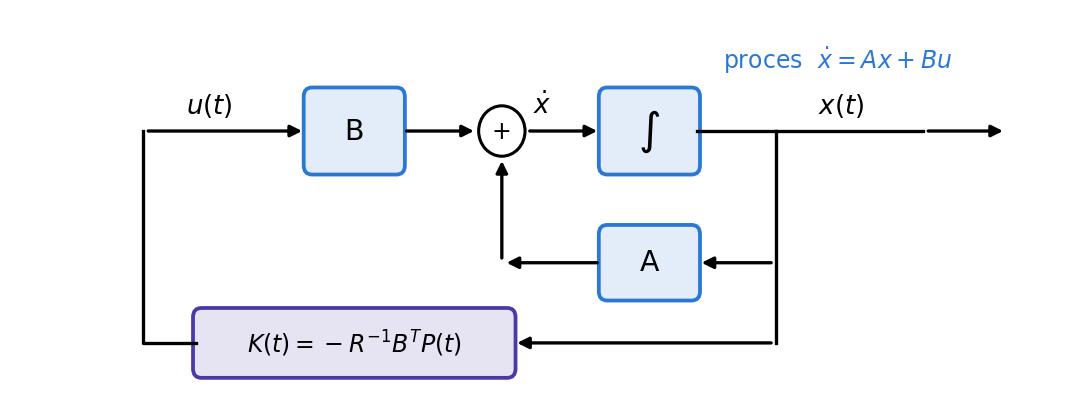
\includegraphics[width=0.7\linewidth,height=\textheight,keepaspectratio,alt={Struktura LQR regulatora. Proces ẋ = Ax + Bu je zatvoren povratnom spregom po celom vektoru stanja preko pojačanja K(t) iz formule iznad, koje se izračuna unapred iz Rikatijeve jednačine.}]{figures/q10_lqr_blok.png}
\caption{Struktura LQR regulatora. Proces ẋ = Ax + Bu je zatvoren povratnom spregom po celom vektoru stanja preko pojačanja K(t) iz formule iznad, koje se izračuna unapred iz Rikatijeve jednačine.}
\end{figure}

\subsection{Stacionarni slučaj}

Profesor navodi tri Kalmanova uslova \izvor{P14 snimak, 60.--63. min; OptControl2022 sl. 27}: (1) sistem je upravljiv; (2) kriterijum je u strogo Lagranžovoj formi (\(\Psi = 0\)); (3) \(A, B, Q, R\) su vremenski nepromenljive. Tada se gornja granica posmatra kao beskonačna (\(t_1 \to \infty\)), a rešenje Rikatijeve jednačine (integraljeno unazad) se ustali: \(P(t) \to P = \text{const}\). Tada je \(\dot P = 0\) i ostaje \textbf{algebarska} Rikatijeva jednačina:

\[A^TP + PA - PBR^{-1}B^TP + Q = 0, \qquad K = -R^{-1}B^TP = \text{const} .\]

To je regulator sa konstantnim pojačanjem, koji se u praksi najčešće koristi (MATLAB \texttt{lqr}). Profesor ovaj slučaj zove najvažnijim za primenu u automatici („ponavljam po stoti put''): vremenski promenljivo pojačanje je teško ili skoro nemoguće napraviti, a konstantno je samo jedno pojačanje u povratnoj sprezi \izvor{P14 snimak, 58.--64. min}.

\subsection{Primer: skalarni stacionarni LQR}

\(\dot x = ax + bu\), \(t_1 \to \infty\). Algebarska jednačina:

\[2aP - \frac{b^2}{r}P^2 + q = 0 \;\Rightarrow\; P = \frac{r}{b^2}\Big(a + \sqrt{a^2 + \frac{b^2q}{r}}\Big) \quad(\text{uzima se } P \ge 0) .\]

Pojačanje i pol zatvorene sprege:

\[K = -\frac{b}{r}P = -\frac1b\Big(a + \sqrt{a^2 + \frac{b^2q}{r}}\Big), \qquad a + bK = -\sqrt{a^2 + \frac{b^2q}{r}} < 0 .\]

\textbf{Zaključak:} pol zatvorene sprege je uvek levo, i kad je sistem nestabilan (\(a > 0\)). Za \(a = b = q = r = 1\): \(P = 1 + \sqrt2 = 2{,}414\), \(K = -2{,}414\), pol \(-\sqrt2\). Povećanje \(q/r\) pomera pol dalje ulevo (brži regulator, veće upravljanje).

Specijalan slučaj \(q = 0\) (prvi primer sa prezentacije, pitanje 12): \(P = \frac{r}{b^2}(a + |a|)\). Za stabilan sistem (\(a < 0\)) je \(P = 0\) i regulator ništa ne radi, jer se ne kažnjava stanje, a sistem se sam smiruje. Za nestabilan (\(a > 0\)) je \(P = 2ar/b^2\) i pol se preslikava u \(-a\). Oprez: jednačina \(2aP - \frac{b^2}{r}P^2 = 0\) ima i rešenje \(P = 0\). Integracija unazad teži ka \(2ar/b^2\) samo ako je \(\Psi > 0\) (kao u pitanju 12); za \(q = 0\) i \(\Psi = 0\) ostaje \(P \equiv 0\), jer se tada ništa ne kažnjava, pa nestabilnost „ne košta''. Zato opšti uslov za stabilnu zatvorenu spregu, pored upravljivosti para \((A, B)\), traži da \(Q\) „vidi'' nestabilne modove (opservabilnost para \((A, Q^{1/2})\)).

\begin{ispit}[{Pitanje 10}]
\begin{itemize}
\item Profesor: „Primenu HJB na linearne sisteme morate da znate da izvedete ... za \textbf{jednokomponentni} slučaj, do Rikatijeve jednačine. Ne insistiram na višekomponentnom'' \izvor{P14 snimak, 43. i 50. min}. Skalarno izvođenje je jezgro odgovora; matrični oblik je dodatak.
\item Obavezno: postavka, \(u = -r^{-1}bp\), \(H^*\), HJB sa \(p = \partial S/\partial x\), pretpostavka \(S = \frac12Px^2\) sa obrazloženjem, Rikatijeva jednačina, \(P(t_1) = \Psi\), \(K(t)\).
\item Napisati i matrični oblik i nacrtati blok dijagram.
\item Reći: \(P\) se računa unazad; uz tri Kalmanova uslova (upravljivost, \(\Psi = 0\), konstantne matrice) i \(t_1 \to \infty\) dobija se algebarska Rikatijeva jednačina i konstantno \(K\).
\item Zamka: pogrešan znak u \(H^*\) (\(-\frac12b^2r^{-1}p^2\)), zaboravljen faktor \(\frac12\) u \(S\).
\end{itemize}
\end{ispit}

\subsection{Moguća potpitanja}

\begin{itemize}
\item \textbf{Zašto baš \(S = \frac12Px^2\)?} Krajnji uslov je kvadratan, a HJB sadrži samo \(x^2\), \(x\,\partial S/\partial x\) i \((\partial S/\partial x)^2\); sa kvadratnim \(S\) svi članovi su \(\sim x^2\), pa se PDJ svodi na ODJ za \(P(t)\). Pretpostavka daje rešenje HJB, a ono je jedinstveno, pa je to pravo rešenje.
\item \textbf{Zašto Rikatijeva jednačina ima rešenje na celom \([t_0, t_1]\)?} Kvadratna jednačina bi mogla „pobeći'' u beskonačno, ali ovde je \(\frac12x^TP(t)x = S(t, x)\) optimalna cena: ona je \(\ge 0\) (jer \(Q, \Psi \ge 0\), \(R > 0\)) i nije veća od cene za \(u \equiv 0\), koja je konačna. Zato je \(P(t)\) ograničeno i postoji do \(t_0\).
\item \textbf{Zašto se \(P\) računa unazad?} Poznat je samo krajnji uslov \(P(t_1) = \Psi\) (iz \(S(t_1, x) = \Psi(x)\)).
\item \textbf{Zašto je \(P\) simetrično i \(\ge 0\)?} Samo simetrični deo matrice utiče na \(x^TPx\), pa se uzima simetričan; \(\ge 0\) jer je to cena.
\item \textbf{Šta rade \(q\) i \(r\)?} Veće \(q/r\): pol dalje ulevo, brži regulator, veće upravljanje. Množenje \(Q\) i \(R\) istim brojem ne menja \(K\).
\item \textbf{Kada je stacionarna zatvorena sprega stabilna?} Kad je \((A, B)\) upravljivo (stabilizabilno) i \(Q\) „vidi'' nestabilne modove; tada je \(a + bK = -\sqrt{a^2 + b^2q/r} < 0\) i za nestabilno \(a\).
\end{itemize}

\section{11. LQR dobijen primenom principa maksimuma}

Zvaničan tekst: \emph{Linearni regulatori sa kvadratnim kriterijumom optimalnosti (LQR), dobijeni primenom principa maksimuma.}

\begin{kljucna}[{Odgovor u 60 sekundi}]
\begin{enumerate}
\def\labelenumi{\arabic{enumi}.}
\item Isti problem kao u pitanju 10: \(\dot x = ax + bu\), \(I = \frac12\Psi x^2(t_1) + \frac12\int(qx^2 + ru^2)dt\).
\item \(H = \frac12(qx^2 + ru^2) + p(ax + bu)\), \(u_{opt} = -r^{-1}bp\), \(H^* = \frac12qx^2 + pax - \frac12b^2r^{-1}p^2\).
\item Kanonske jednačine: \(\dot x = \partial H^*/\partial p = ax - b^2r^{-1}p\), \(\dot p = -\partial H^*/\partial x = -qx - ap\); uslovi \(x(t_0) = x_0\) i (Bolca) \(p(t_1) = \Psi x(t_1)\).
\item Sistem je linearan i krajnji uslov je linearan, pa se pretpostavlja \(p(t) = P(t)x(t)\).
\item Diferenciranjem \(\dot p = \dot Px + P\dot x\) i zamenom obe kanonske jednačine: \((\dot P + 2aP - b^2r^{-1}P^2 + q)x = 0\).
\item Dobija se ista Rikatijeva jednačina kao iz HJB, \(P(t_1) = \Psi\), i \(u_{opt} = -r^{-1}bP(t)x(t)\): zatvorena sprega, iako Pontrjagin inače daje otvorenu.
\end{enumerate}
\end{kljucna}

\subsection{Ideja}

Princip maksimuma inače daje upravljanje kao funkciju vremena, \(u^*(t)\), za jedan početni uslov. Kod LQR je dvotačkasti problem \textbf{linearan}, pa je veza između \(p\) i \(x\) u svakom trenutku linearna: \(p(t) = P(t)x(t)\). Kad se to uvrsti u \(u = -r^{-1}bp\), dobija se povratna sprega po stanju. Tako i Pontrjaginov put vodi do iste Rikatijeve jednačine kao Belmanov.

\subsection{Postavka}

\[\dot x = ax + bu, \qquad x(t_0) = x_0, \qquad t_0 \le t \le t_1, \qquad I = \frac12\Psi x^2(t_1) + \frac12\int_{t_0}^{t_1}\big(qx^2 + ru^2\big)dt\]

\(r > 0\), \(q \ge 0\), \(\Psi \ge 0\) (obrazloženje u pitanju 10) \izvor{OptControl2022 sl. 18--20}.

\subsection{Izvođenje}

\textbf{Korak 1: Hamiltonijan i upravljanje.}

\[H = \frac12\big(qx^2 + ru^2\big) + p(ax + bu), \qquad \frac{\partial H}{\partial u} = ru + bp = 0 \;\Rightarrow\; u_{opt} = -r^{-1}b\,p(t) .\]

\(\partial^2H/\partial u^2 = r > 0\), pa je to minimum.

\textbf{Korak 2: \(H^*\).} Uvrštavanjem (isti račun kao u pitanju 10):

\[H^* = \frac12qx^2 + pax - \frac12b^2r^{-1}p^2 .\]

\textbf{Korak 3: kanonske jednačine.}

\[\dot x = \frac{\partial H^*}{\partial p} = ax - b^2r^{-1}p(t), \qquad \dot p = -\frac{\partial H^*}{\partial x} = -qx - a\,p(t) .\]

(Na slajdu 18 u imeniocu druge jednačine piše \(\partial p\); mora biti \(\partial x\), kao na slajdu 19.)

\textbf{Korak 4: granični uslovi.} \(x(t_0) = x_0\) je zadato. Kraj je slobodan, a kriterijum je Bolcin sa \(\Psi(x) = \frac12\Psi x^2\), pa je (pitanje 3)

\[p(t_1) = \frac{\partial}{\partial x(t_1)}\Big(\frac12\Psi x^2(t_1)\Big) = \Psi\,x(t_1) .\]

To je dvotačkasti problem: \(x\) je zadato na početku, \(p\) na kraju.

\textbf{Korak 5: zašto \(p = P(t)x\).} Kanonske jednačine su linearne. U matričnom obliku:

\[\frac{d}{dt}\begin{bmatrix} x \\ p \end{bmatrix} = \begin{bmatrix} a & -b^2r^{-1} \\ -q & -a \end{bmatrix}\begin{bmatrix} x \\ p \end{bmatrix} .\]

Neka je \(\Phi(t_1, t)\) prelazna matrica ovog sistema, sa blokovima \(\Phi_{11}, \Phi_{12}, \Phi_{21}, \Phi_{22}\). Tada je \(x(t_1) = \Phi_{11}x(t) + \Phi_{12}p(t)\) i \(p(t_1) = \Phi_{21}x(t) + \Phi_{22}p(t)\). Uslov \(p(t_1) = \Psi x(t_1)\) daje

\[\Phi_{21}x + \Phi_{22}p = \Psi\big(\Phi_{11}x + \Phi_{12}p\big) \;\Rightarrow\; p(t) = \big(\Phi_{22} - \Psi\Phi_{12}\big)^{-1}\big(\Psi\Phi_{11} - \Phi_{21}\big)\,x(t) .\]

Koeficijent zavisi samo od \(t\) (preko \(\Phi(t_1, t)\)), a ne od \(x_0\). (Inverz postoji za \(Q, \Psi \ge 0\), \(R > 0\): to je isto tvrđenje kao da Rikatijeva jednačina nema bekstvo u beskonačno, v. potpitanja pitanja 10.) Označi se sa \(P(t)\):

\[p(t) = P(t)\,x(t), \qquad P(t_1) = \Psi \quad(\text{iz } p(t_1) = \Psi x(t_1)) .\]

Na slajdu je ovaj korak samo „pretpostavka'' (uokviren izraz \(p = Px\)), a gornji račun pokazuje zašto ona važi.

\textbf{Korak 6: jednačina za \(P\).} Izvod proizvoda:

\[\dot p(t) = \dot P(t)\,x(t) + P(t)\,\dot x(t) .\]

Leva strana iz druge kanonske jednačine, a \(\dot x\) iz prve, sa \(p = Px\):

\[-qx - aPx = \dot Px + P\big(ax - b^2r^{-1}Px\big) = \dot Px + aPx - b^2r^{-1}P^2x .\]

Sve se prebaci na jednu stranu:

\[\big(\dot P + 2aP - b^2r^{-1}P^2 + q\big)\,x = 0 .\]

Ovo važi za svako \(x\) (za svaki početni uslov), pa je zagrada nula.

\begin{kljucna}
\[\dot P + 2aP - b^2r^{-1}P^2 + q = 0, \qquad P(t_1) = \Psi\]

\[u_{opt} = -r^{-1}b\,P(t)\,x(t) = K(t)\,x(t), \qquad K(t) = -r^{-1}bP(t)\]

Ista jednačina kao iz HJB (pitanje 10). Ovde je \(P(t)\) koeficijent veze \(p = Px\), a tamo koeficijent kvadratne forme \(S = \frac12Px^2\). Veza je \(p = \partial S/\partial x = Px\).
\end{kljucna}

\subsection{Matrični oblik}

Za \(\dot x = Ax + Bu\) i \(I = \frac12x^T(t_1)\Psi x(t_1) + \frac12\int(x^TQx + u^TRu)dt\):

\textbf{Korak 1.} \(H = \frac12(x^TQx + u^TRu) + p^T(Ax + Bu)\), \(u = -R^{-1}B^Tp\).

\textbf{Korak 2.} Kanonske jednačine: \(\dot x = Ax - BR^{-1}B^Tp\), \(\dot p = -\frac{\partial H}{\partial x} = -Qx - A^Tp\), uz \(p(t_1) = \Psi x(t_1)\).

\textbf{Korak 3.} \(p = P(t)x\), \(\dot p = \dot Px + P\dot x\):

\[-Qx - A^TPx = \dot Px + PAx - PBR^{-1}B^TPx \;\Rightarrow\; \big(\dot P + A^TP + PA - PBR^{-1}B^TP + Q\big)x = 0 .\]

\[\dot P + A^TP + PA - PBR^{-1}B^TP + Q = 0, \qquad P(t_1) = \Psi, \qquad u_{opt} = K(t)x, \qquad K(t) = -R^{-1}B^TP(t) .\]

\subsection{Primer: sopstvene vrednosti Hamiltonove matrice}

Za \(t_1 \to \infty\) i konstantne koeficijente stacionarno rešenje ima lepu vezu sa matricom iz koraka 5. Za \(a = b = q = r = 1\):

\[\frac{d}{dt}\begin{bmatrix} x \\ p \end{bmatrix} = \begin{bmatrix} 1 & -1 \\ -1 & -1 \end{bmatrix}\begin{bmatrix} x \\ p \end{bmatrix}, \qquad \det\begin{bmatrix} 1 - s & -1 \\ -1 & -1 - s \end{bmatrix} = s^2 - 2 = 0 \;\Rightarrow\; s = \pm\sqrt2 .\]

Opšte: \(s^2 - a^2 - b^2q/r = 0\), tj. \(s = \pm\sqrt{a^2 + b^2q/r}\). Sopstvene vrednosti dolaze u paru \(\pm s\).

\textbf{Stacionarni \(P\) i pol} (primer iz pitanja 10): iz \(\dot P = 0\) je \(2P - P^2 + 1 = 0\), \(P = 1 + \sqrt2\), \(K = -(1 + \sqrt2)\), pa je \(\dot x = (a + bK)x = -\sqrt2\,x\). To je baš \textbf{stabilna} sopstvena vrednost Hamiltonove matrice. Na optimalnoj putanji je \(p = Px\), pa se kreće samo stabilni mod; nestabilni (\(+\sqrt2\)) je „isključen'' graničnim uslovom.

\subsection{Poređenje dva puta do LQR}

\begin{longtable}[]{@{}
  >{\raggedright\arraybackslash}p{(\linewidth - 4\tabcolsep) * \real{0.2143}}
  >{\raggedright\arraybackslash}p{(\linewidth - 4\tabcolsep) * \real{0.4375}}
  >{\raggedright\arraybackslash}p{(\linewidth - 4\tabcolsep) * \real{0.3482}}@{}}
\caption{Dva izvođenja LQR \izvor{OptControl2022 sl. 17--21, 31--33}}\tabularnewline
\toprule\noalign{}
\begin{minipage}[b]{\linewidth}\raggedright
\end{minipage} & \begin{minipage}[b]{\linewidth}\raggedright
Pontrjagin (pitanje 11)
\end{minipage} & \begin{minipage}[b]{\linewidth}\raggedright
Belman (pitanje 10)
\end{minipage} \\
\midrule\noalign{}
\endfirsthead
\toprule\noalign{}
\begin{minipage}[b]{\linewidth}\raggedright
\end{minipage} & \begin{minipage}[b]{\linewidth}\raggedright
Pontrjagin (pitanje 11)
\end{minipage} & \begin{minipage}[b]{\linewidth}\raggedright
Belman (pitanje 10)
\end{minipage} \\
\midrule\noalign{}
\endhead
\bottomrule\noalign{}
\endlastfoot
Polazna tačka & kanonske jednačine za \(x\) i \(p\) & HJB parcijalna jednačina za \(S(t, x)\) \\
Ključna pretpostavka & \(p(t) = P(t)x(t)\) & \(S(t, x) = \frac12P(t)x^2\) \\
Krajnji uslov & \(p(t_1) = \Psi x(t_1)\) & \(S(t_1, x) = \frac12\Psi x^2\) \\
Rezultat & \(\dot P + 2aP - b^2r^{-1}P^2 + q = 0\), \(P(t_1) = \Psi\) & ista jednačina \\
\end{longtable}

\begin{ispit}[{Pitanje 11}]
\begin{itemize}
\item Kanonske jednačine sa \(H^*\) i granični uslov \(p(t_1) = \Psi x(t_1)\) (Bolca) su polazna tačka.
\item Ključni korak: \(p = Px\), pa \(\dot p = \dot Px + P\dot x\) i zamena obe kanonske jednačine. Ako se pita „zašto \(p = Px\)„, odgovor je linearnost dvotačkastog problema (prelazna matrica).
\item Reći da je rezultat ista Rikatijeva jednačina kao iz HJB i da je upravljanje u zatvorenoj sprezi.
\item Zamka: u \(\dot p\) znak minus ispred \(\partial H/\partial x\); lako se dobije \(-2aP\) umesto \(+2aP\).
\end{itemize}
\end{ispit}

\subsection{Moguća potpitanja}

\begin{itemize}
\item \textbf{Zašto sme \(p = P(t)x\)?} Kanonske jednačine i uslov \(p(t_1) = \Psi x(t_1)\) su linearni, pa preko prelazne matrice \(p(t)\) ispada linearna funkcija od \(x(t)\), sa koeficijentom koji ne zavisi od \(x_0\) (korak 5).
\item \textbf{Kako Pontrjagin ovde daje zatvorenu spregu?} Sam princip daje \(u(t) = -r^{-1}bp(t)\); tek zamena \(p = Px\) pretvara to u \(u = K(t)x\). To je moguće samo zato što je problem linearno-kvadratni.
\item \textbf{Zašto je ovde potreban uslov i dovoljan?} Sistem je linearan, a kriterijum konveksan (\(q, \Psi \ge 0\), \(r > 0\)), pa je stacionarna tačka jedinstveni globalni minimum.
\item \textbf{Zašto sopstvene vrednosti Hamiltonove matrice dolaze u paru \(\pm s\)?} Karakteristični polinom je \(s^2 - (a^2 + b^2q/r)\), paran po \(s\); u matričnom slučaju važi isto zbog strukture matrice. Optimalna zatvorena sprega uzima stabilnu polovinu.
\item \textbf{Šta ako je \(x(t_1) = 0\) zadato?} Tada \(p(t_1)\) nije poznato; to odgovara \(\Psi \to \infty\), tj. \(P(t_1) = \infty\). Praktično se uzme veliko \(\Psi\) (kao u FBSM, pitanje 6).
\item \textbf{Po čemu se razlikuje \(P\) ovde i u pitanju 10?} Samo po tumačenju: ovde je koeficijent veze \(p = Px\), tamo koeficijent kvadratne forme \(S = \frac12Px^2\); kako je \(p = \partial S/\partial x\), to je ista funkcija.
\end{itemize}

\section{12. LQR: rezultati simulacija tri primera sa prezentacije}

Zvaničan tekst: \emph{Linearni regulatori sa kvadratnim kriterijumom optimalnosti (LQR), rezultati simulacija tri primera sa prezentacije.}

Primeri su sa slajdova 22--30 \izvor{OptControl2022}. Sve simulacije su ponovljene (\texttt{skripte/\allowbreak{}numerika.py}, Rikatijeva jednačina integraljena unazad sa \texttt{solve\_ivp}, stacionarni slučaj sa \texttt{solve\_\allowbreak{}continuous\_\allowbreak{}are}), a brojevi su upoređeni sa slajdovima.

\begin{kljucna}[{Odgovor u 60 sekundi}]
\begin{enumerate}
\def\labelenumi{\arabic{enumi}.}
\item Primer 1: skalarni sistem \(\dot x = ax + u\), \(I = \frac12\Psi x^2(T) + \int\frac14u^2dt\), \(T = 15\) s, \(a = \pm0{,}2\), tri vrednosti \(\Psi\). Rikatijeva jednačina je \(\dot P = 2P^2 - 2aP\), \(P(T) = \Psi\), \(u = -2Px\).
\item Za stabilan sistem (\(a = -0{,}2\)) \(P \approx 0\) skoro ceo interval: regulator skoro ništa ne radi, pa se sistem smiruje sam, a tek pred kraj \(P\) skače ka \(\Psi\).
\item Za nestabilan (\(a = 0{,}2\)) \(P \approx a = 0{,}2\) skoro ceo interval, pa je \(u(0) \approx -2\); \(\Psi\) utiče samo na kraj.
\item Primer 2: sistem drugog reda (jedan nestabilan pol), \(\Psi = 0\): \(P(t)\) je konstantno do blizu kraja, pa je \(K\) praktično konstantno; stanja idu u nulu za oko 4 s.
\item Primer 3: obrnuto klatno na kolicima, 4 stanja, stacionarni LQR: polovi \(\pm3{,}28\) i \(0, 0\) se premeštaju u \(-4{,}41\), \(-2{,}48\), \(-0{,}60 \pm 0{,}45i\); klatno se uspravi za oko 2 s, a kolica se vrate za oko 7 s.
\item Zajednička poruka: \(P(t)\) se računa unazad, ustali se daleko od kraja, a \(\Psi\) utiče samo na kraj intervala.
\end{enumerate}
\end{kljucna}

\subsection{Ideja}

Tri primera pokazuju tri stvari. Prvi pokazuje kako izgleda rešenje Rikatijeve jednačine u vremenu i šta radi težina \(\Psi\). Drugi pokazuje da se za dug interval \(P(t)\) ustali, pa vremenski promenljivo pojačanje postaje konstantno. Treći je realan višedimenzionalni problem (stabilizacija obrnutog klatna), gde se koristi direktno stacionarni regulator.

Formule koje se koriste (pitanja 10 i 11), za \(I = \frac12x^T(T)\Psi x(T) + \frac12\int(x^TQx + u^TRu)dt\):

\[\dot P = -A^TP - PA + PBR^{-1}B^TP - Q, \qquad P(T) = \Psi, \qquad u = -R^{-1}B^TP(t)\,x .\]

\subsection{\texorpdfstring{Primer 1: skalarni sistem, uticaj \(a\) i \(\Psi\)}{Primer 1: skalarni sistem, uticaj a i \textbackslash Psi}}

\textbf{Postavka} \izvor{OptControl2022 sl. 22}:

\[\dot x = ax + u, \qquad x(0) = 5, \qquad T = 15 \text{ s}, \qquad I = \frac12\Psi x^2(T) + \int_0^T\frac14u^2\,dt, \qquad a = \pm0{,}2, \quad \Psi \in \{5;\ 0{,}5;\ 0{,}05\} .\]

(Na graficima slajda težina je označena sa „H'', a u tekstu je to \(\Psi\).)

\textbf{Svođenje na opšti oblik.} \(\int\frac14u^2 = \frac12\int\frac12u^2\), pa je \(r = \frac12\), \(q = 0\), \(b = 1\).

\textbf{Rikatijeva jednačina i upravljanje.} \(H = \frac14u^2 + p(ax + u)\), \(\frac{\partial H}{\partial u} = \frac12u + p = 0\), pa je \(u_{opt} = -2p = -2P(t)x(t)\). Iz \(\dot P + 2aP - b^2r^{-1}P^2 + q = 0\):

\[\dot P = 2P^2 - 2aP, \qquad P(T) = \Psi .\]

\textbf{Analitičko rešenje} (za proveru). Smena \(z = 1/P\): \(\dot z = -\dot P/P^2 = -2 + 2az\). Rešenje linearne jednačine je \(z = \frac1a + Ce^{2at}\), a iz \(z(T) = 1/\Psi\):

\[P(t) = \frac{1}{\dfrac1a + \Big(\dfrac1\Psi - \dfrac1a\Big)e^{2a(t - T)}} .\]

\begin{itemize}
\item \(a = 0{,}2\): daleko od kraja je \(e^{2a(t - T)} \approx 0\), pa je \(P \approx a = 0{,}2\) i \(u(0) \approx -2\cdot0{,}2\cdot5 = -2\).
\item \(a = -0{,}2\): \(e^{2a(t - T)} = e^{0{,}4(T - t)}\) je ogromno daleko od kraja, pa je \(P \approx 0\) i \(u \approx 0\).
\end{itemize}

Ovo se slaže sa stacionarnim rezultatom iz pitanja 10 za \(q = 0\): \(P = \frac{r}{b^2}(a + |a|)\).

\begin{figure}
\centering
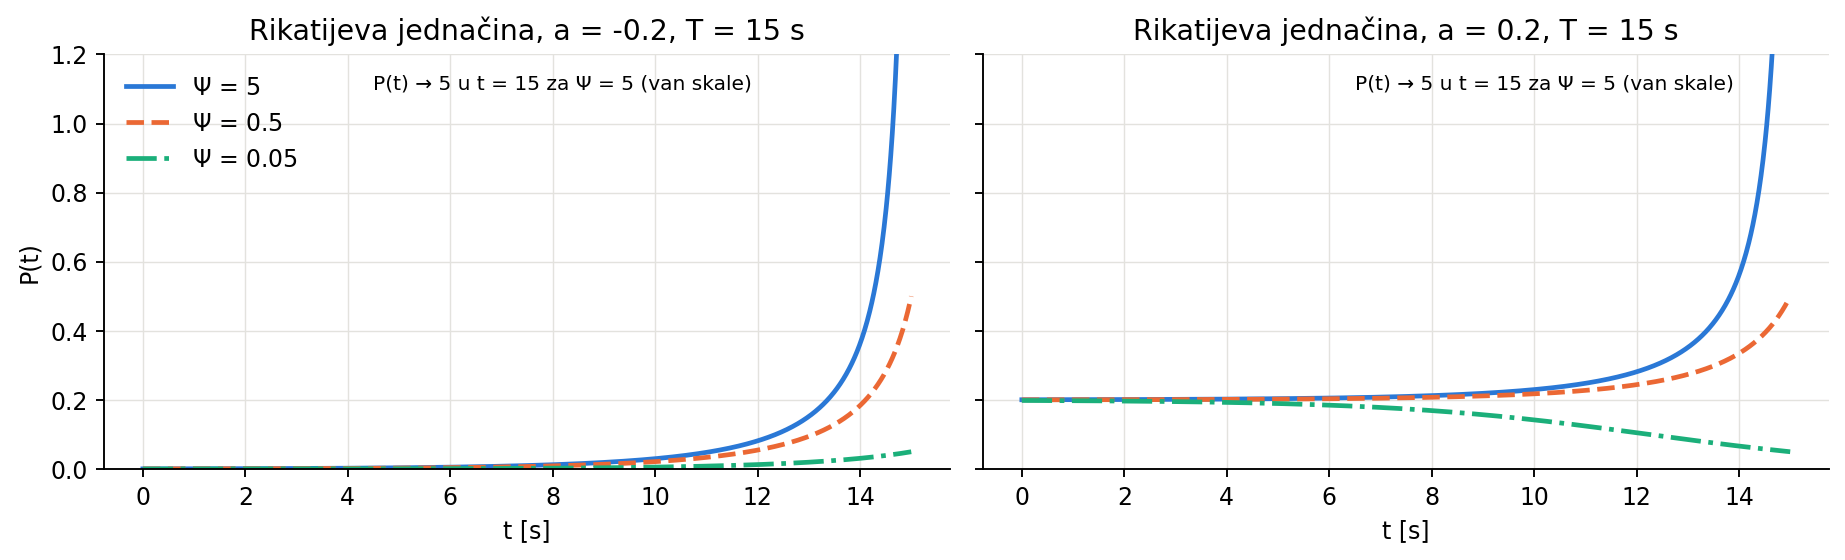
\includegraphics[width=0.95\linewidth,height=\textheight,keepaspectratio,alt={Primer 1: rešenja Rikatijeve jednačine (računata unazad od P(15) = Ψ). Za a = −0,2 P je praktično nula do pred kraj. Za a = 0,2 P se ustali na a = 0,2, a Ψ menja samo poslednjih nekoliko sekundi.}]{figures/q12_pr1_P.png}
\caption{Primer 1: rešenja Rikatijeve jednačine (računata unazad od P(15) = Ψ). Za a = −0,2 P je praktično nula do pred kraj. Za a = 0,2 P se ustali na a = 0,2, a Ψ menja samo poslednjih nekoliko sekundi.}
\end{figure}

\begin{figure}
\centering
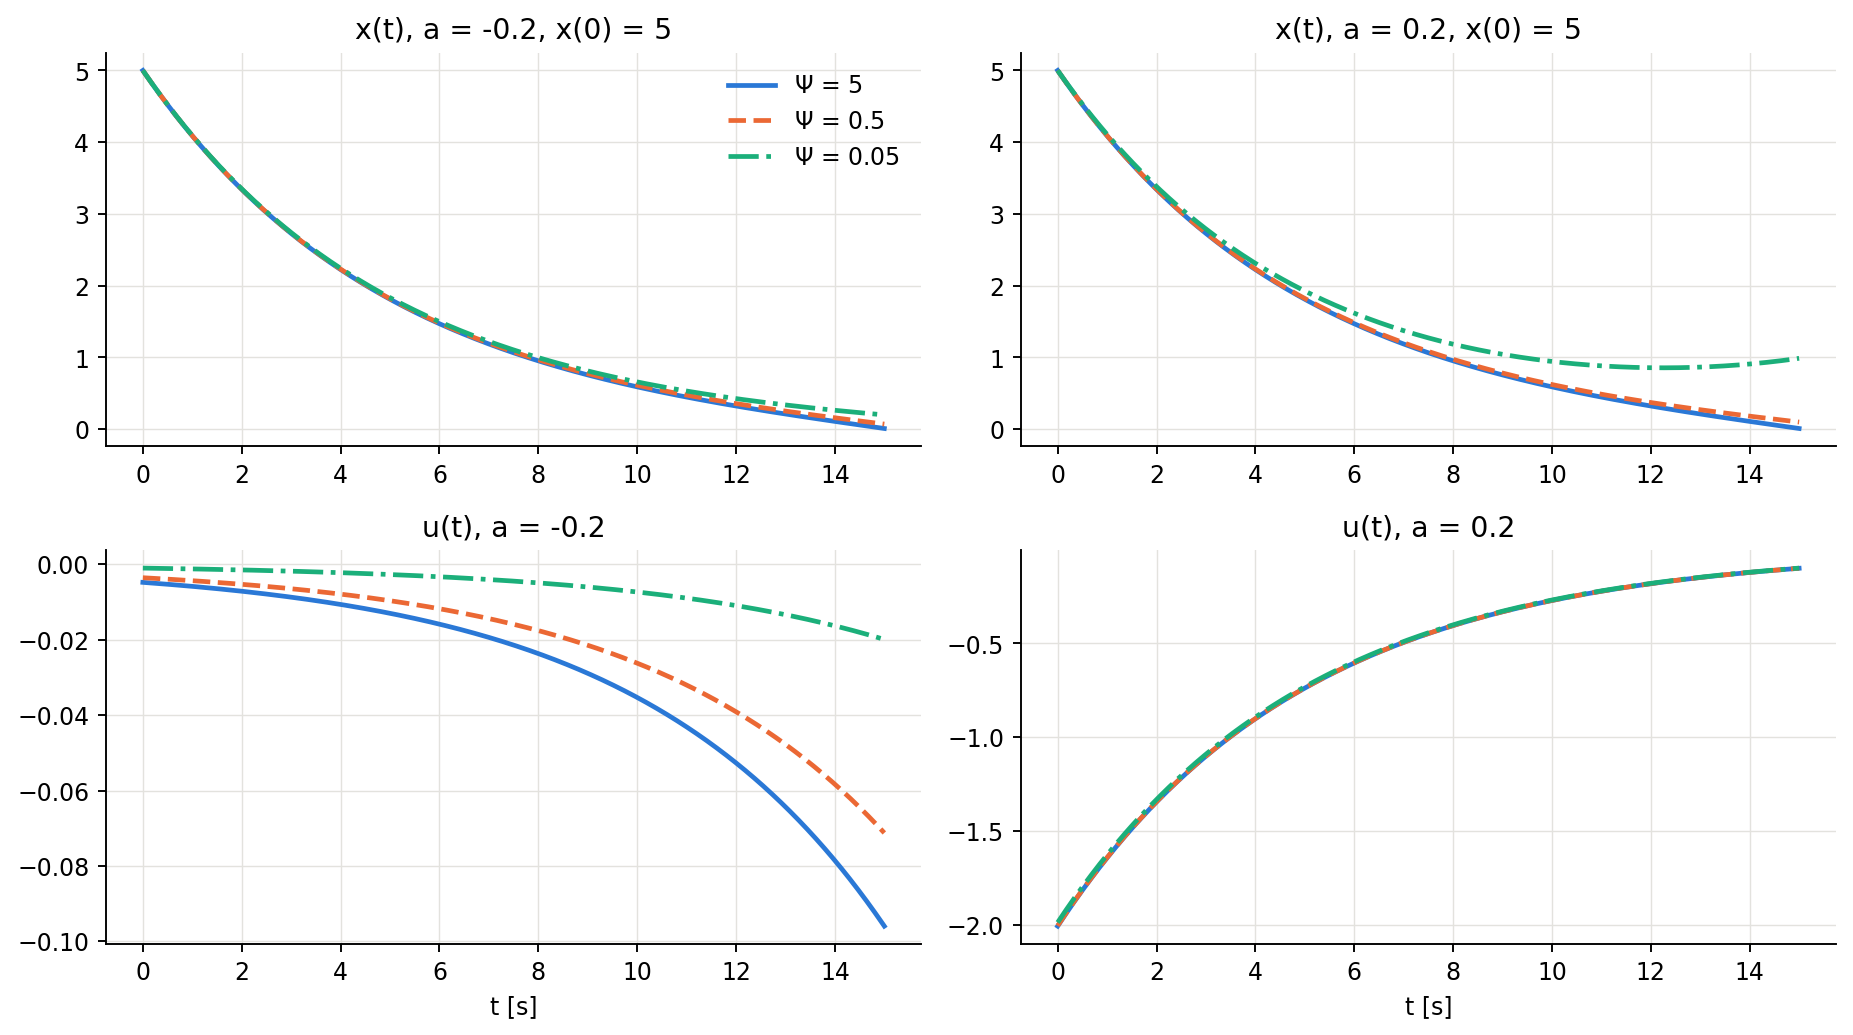
\includegraphics[width=0.95\linewidth,height=\textheight,keepaspectratio,alt={Primer 1: stanje i upravljanje. Levo (a = −0,2): stanje opada skoro kao 5e\^{}(−0,2t), upravljanje je malo i raste tek pri kraju. Desno (a = 0,2): upravljanje na početku iznosi −2 i pretvara nestabilan pol +0,2 u −0,2; za malo Ψ = 0,05 povratna sprega pred kraj slabi, pa nestabilan sistem ponovo raste.}]{figures/q12_pr1_xu.png}
\caption{Primer 1: stanje i upravljanje. Levo (a = −0,2): stanje opada skoro kao 5e\^{}(−0,2t), upravljanje je malo i raste tek pri kraju. Desno (a = 0,2): upravljanje na početku iznosi −2 i pretvara nestabilan pol +0,2 u −0,2; za malo Ψ = 0,05 povratna sprega pred kraj slabi, pa nestabilan sistem ponovo raste.}
\end{figure}

\begin{longtable}[]{@{}ccrrrr@{}}
\caption{Primer 1, brojevi iz simulacije; provereno i nezavisnim rešavanjem}\tabularnewline
\toprule\noalign{}
\(a\) & \(\Psi\) & \(P(0)\) & \(u(0)\) & \(x(T)\) & \(u(T)\) \\
\midrule\noalign{}
\endfirsthead
\toprule\noalign{}
\(a\) & \(\Psi\) & \(P(0)\) & \(u(0)\) & \(x(T)\) & \(u(T)\) \\
\midrule\noalign{}
\endhead
\bottomrule\noalign{}
\endlastfoot
−0,2 & 5 & 0,0005 & −0,005 & 0,010 & −0,096 \\
−0,2 & 0,5 & 0,0004 & −0,004 & 0,071 & −0,071 \\
−0,2 & 0,05 & 0,0001 & −0,001 & 0,199 & −0,020 \\
0,2 & 5 & 0,2005 & −2,005 & 0,010 & −0,100 \\
0,2 & 0,5 & 0,2003 & −2,003 & 0,100 & −0,100 \\
0,2 & 0,05 & 0,1985 & −1,985 & 0,988 & −0,099 \\
\end{longtable}

\textbf{Šta reći.}

\begin{itemize}
\item \(\Psi\) je kazna za krajnje stanje: veće \(\Psi\) daje manje \(x(T)\). Bez člana \(q x^2\) samo \(\Psi\) „tera'' stanje u nulu.
\item Stabilan sistem: regulator se ne troši dok sistem sam ide ka nuli (upravljanje reda \(10^{-3}\)), a interveniše tek pri kraju.
\item Nestabilan sistem: regulator mora da radi celo vreme, sa praktično konstantnim pojačanjem \(K = -2P = -0{,}4\).
\item \(P(t)\) ima oblik „ravno pa skok pri kraju'': zato se za duge intervale koristi konstantno pojačanje.
\item Profesorova rečenica: „optimalno upravljanje je za nestabilan sistem najveće na početku, a za stabilan na kraju, kad treba da ga smiri'' \izvor{P14 snimak, 57. min}.
\end{itemize}

\subsection{\texorpdfstring{Primer 2: sistem drugog reda, \(\Psi = 0\)}{Primer 2: sistem drugog reda, \textbackslash Psi = 0}}

\textbf{Postavka} \izvor{OptControl2022 sl. 26--27}:

\[\dot x_1 = x_2, \qquad \dot x_2 = 2x_1 - x_2 + u, \qquad I = \int_0^T\Big(x_1^2 + \frac12x_2^2 + \frac14u^2\Big)dt, \qquad T = 15 \text{ s}, \qquad x(0) = (-4, 4) .\]

\[H = x_1^2 + \frac12x_2^2 + \frac14u^2 + p_1x_2 + p_2(2x_1 - x_2 + u), \qquad u_{opt} = -2p_2 = -2\big[P_{12}(t)\;\; P_{22}(t)\big]x .\]

\textbf{Matrice.} \(A = \begin{bmatrix} 0 & 1 \\ 2 & -1\end{bmatrix}\), \(B = \begin{bmatrix} 0 \\ 1\end{bmatrix}\). Kriterijum u obliku \(\frac12\int(x^TQx + Ru^2)\) daje \(Q = \operatorname{diag}(2, 1)\), \(R = \frac12\). Sopstvene vrednosti \(A\): \(s^2 + s - 2 = 0\), \(s = 1\) i \(s = -2\), pa je sistem nestabilan.

\textbf{Stacionarni \(P\) ručno} (važi daleko od kraja). Za \(P = \begin{bmatrix} \alpha & \beta \\ \beta & \gamma\end{bmatrix}\) je \(PBR^{-1}B^TP = 2\begin{bmatrix} \beta^2 & \beta\gamma \\ \beta\gamma & \gamma^2\end{bmatrix}\) i \(A^TP + PA = \begin{bmatrix} 4\beta & \alpha - \beta + 2\gamma \\ \alpha - \beta + 2\gamma & 2\beta - 2\gamma\end{bmatrix}\). Algebarska jednačina \(A^TP + PA - PBR^{-1}B^TP + Q = 0\) po elementima:

\[(1,1):\; 4\beta - 2\beta^2 + 2 = 0 \;\Rightarrow\; \beta = 1 + \sqrt2 = 2{,}4142\]

\[(2,2):\; 2\beta - 2\gamma - 2\gamma^2 + 1 = 0 \;\Rightarrow\; \gamma^2 + \gamma - 2{,}9142 = 0 \;\Rightarrow\; \gamma = 1{,}2788\]

\[(1,2):\; \alpha - \beta + 2\gamma - 2\beta\gamma = 0 \;\Rightarrow\; \alpha = 6{,}0313\]

Pažnja na znak: ovde (i u primeru 3) \(K\) je u MATLAB konvenciji, \(K = R^{-1}B^TP\) i \(u = -Kx\) (kao \texttt{lqr}), dok je u pitanjima 10 i 11 \(K = -R^{-1}B^TP\) i \(u = Kx\). Regulator je isti, razlikuje se samo znak u oznaci.

\[K = R^{-1}B^TP = 2\,[\beta\;\; \gamma] = [4{,}828\;\; 2{,}558], \qquad u = -Kx, \qquad u(0) = -(4{,}828\cdot(-4) + 2{,}558\cdot4) = 9{,}08 .\]

\textbf{Zatvorena sprega.} \(A - BK = \begin{bmatrix} 0 & 1 \\ -2{,}828 & -3{,}558\end{bmatrix}\), karakteristični polinom \(s^2 + 3{,}558s + 2{,}828\), polovi \(-1{,}20\) i \(-2{,}36\). Nestabilan pol \(+1\) je premešten ulevo.

Simulacija daje \(P(0) = \begin{bmatrix} 6{,}031 & 2{,}414 \\ 2{,}414 & 1{,}279\end{bmatrix}\), isto kao ručni račun, a na slajdu 27 su vrednosti \(\approx 6\), \(2{,}4\) i \(1{,}3\).

\begin{figure}
\centering
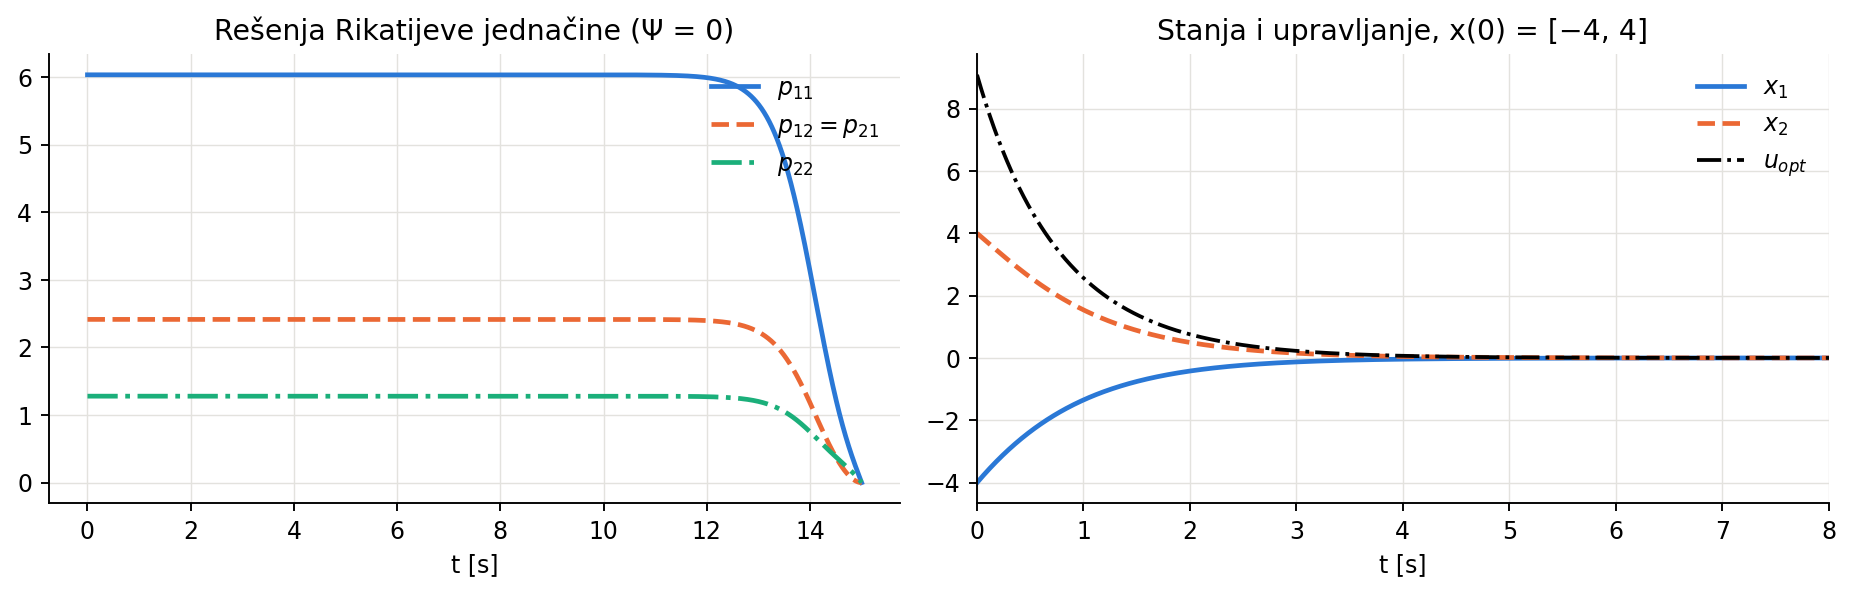
\includegraphics[width=0.95\linewidth,height=\textheight,keepaspectratio,alt={Primer 2. Levo: elementi P(t) su konstantni skoro ceo interval i padaju na nulu tek poslednje 2--3 sekunde (jer je Ψ = 0). Desno: stanja iz (−4, 4) idu u nulu za oko 4 s, a upravljanje kreće od u(0) = 9,1.}]{figures/q12_pr2.png}
\caption{Primer 2. Levo: elementi P(t) su konstantni skoro ceo interval i padaju na nulu tek poslednje 2--3 sekunde (jer je Ψ = 0). Desno: stanja iz (−4, 4) idu u nulu za oko 4 s, a upravljanje kreće od u(0) = 9,1.}
\end{figure}

\textbf{Šta reći} (to je i poruka slajda 27): sistem je upravljiv, \(\Psi = 0\) (Lagranžov problem) i matrice \(A, B, Q, R\) su konstantne, pa \(P(t) \to P\) kad \(t_f \to \infty\). Zato se u praksi koristi konstantno \(K\) iz algebarske Rikatijeve jednačine. Profesor na predavanju: \(P\) je konstantno skoro ceo interval, a stanja se smire mnogo pre nego što \(P\) počne da pada, pa se za taj problem \(P\) može smatrati konstantnim; vremenski promenljivo pojačanje „sa stanovišta automatike nema puno smisla'', jer se teško pravi \izvor{P14 snimak, 58.--61. min}.

Napomena: u nekim zapisima se koristi \(Q = \operatorname{diag}(1;\ 0{,}5)\) i \(R = 0{,}25\), tj. težine bez faktora \(\frac12\). Tada je \(P\) dvaput manje, ali je \(K = R^{-1}B^TP\) isto, pa su i simulacije iste. Množenje \(Q\) i \(R\) istim brojem ne menja regulator.

\subsection{Primer 3: obrnuto klatno na kolicima}

\textbf{Postavka} \izvor{OptControl2022 sl. 28--30}: kolica mase \(M = 5\) kg, klatno mase \(m = 0{,}5\) kg i dužine \(L = 1\) m, sila \(u\) na kolica. Stanje je \(x = [\Theta\;\; \dot\Theta\;\; p\;\; \dot p]^T\) (ugao klatna od vertikale i položaj kolica). Linearizovan model oko uspravnog položaja:

\[\dot x = \begin{bmatrix} 0 & 1 & 0 & 0 \\ 10{,}78 & 0 & 0 & 0 \\ 0 & 0 & 0 & 1 \\ -0{,}98 & 0 & 0 & 0\end{bmatrix}x + \begin{bmatrix} 0 \\ -0{,}2 \\ 0 \\ 0{,}2\end{bmatrix}u, \qquad Q = \operatorname{diag}(100, 100, 10, 10), \quad R = 1, \quad x(0) = [0{,}1\;\; 0\;\; 0{,}1\;\; 0]^T .\]

Brojevi odgovaraju standardnom linearizovanom modelu \(\ddot\Theta = \frac{(M + m)g}{ML}\Theta - \frac{1}{ML}u\), \(\ddot p = -\frac{mg}{M}\Theta + \frac1Mu\), sa \(g = 9{,}8\): \(\frac{5{,}5\cdot9{,}8}{5} = 10{,}78\), \(\frac{0{,}5\cdot9{,}8}{5} = 0{,}98\), \(\frac1{ML} = \frac1M = 0{,}2\). (Model nije izveden na slajdu; ovo je provera koeficijenata.)

\textbf{Rezultat} (stacionarni LQR):

\begin{longtable}[]{@{}
  >{\raggedright\arraybackslash}p{(\linewidth - 2\tabcolsep) * \real{0.3553}}
  >{\raggedright\arraybackslash}p{(\linewidth - 2\tabcolsep) * \real{0.6447}}@{}}
\caption{Primer 3: polovi pre i posle LQR (isto na slajdu 29 i u simulaciji)}\tabularnewline
\toprule\noalign{}
\begin{minipage}[b]{\linewidth}\raggedright
\end{minipage} & \begin{minipage}[b]{\linewidth}\raggedright
sopstvene vrednosti
\end{minipage} \\
\midrule\noalign{}
\endfirsthead
\toprule\noalign{}
\begin{minipage}[b]{\linewidth}\raggedright
\end{minipage} & \begin{minipage}[b]{\linewidth}\raggedright
sopstvene vrednosti
\end{minipage} \\
\midrule\noalign{}
\endhead
\bottomrule\noalign{}
\endlastfoot
bez regulatora (\(A\)) & \(0,\; 0,\; 3{,}2833,\; -3{,}2833\) \\
sa regulatorom (\(A - BK\)) & \(-4{,}4141,\; -2{,}4817,\; -0{,}6018 \pm 0{,}4513i\) \\
\end{longtable}

\(K = [-156{,}2\;\; -49{,}2\;\; -3{,}16\;\; -8{,}72]\) (za \(u = -Kx\)). Otvoren sistem ima pol \(+3{,}28\) (klatno pada) i dvostruki pol u nuli (kolica su dvostruki integrator). LQR sve pomera ulevo.

\begin{figure}
\centering
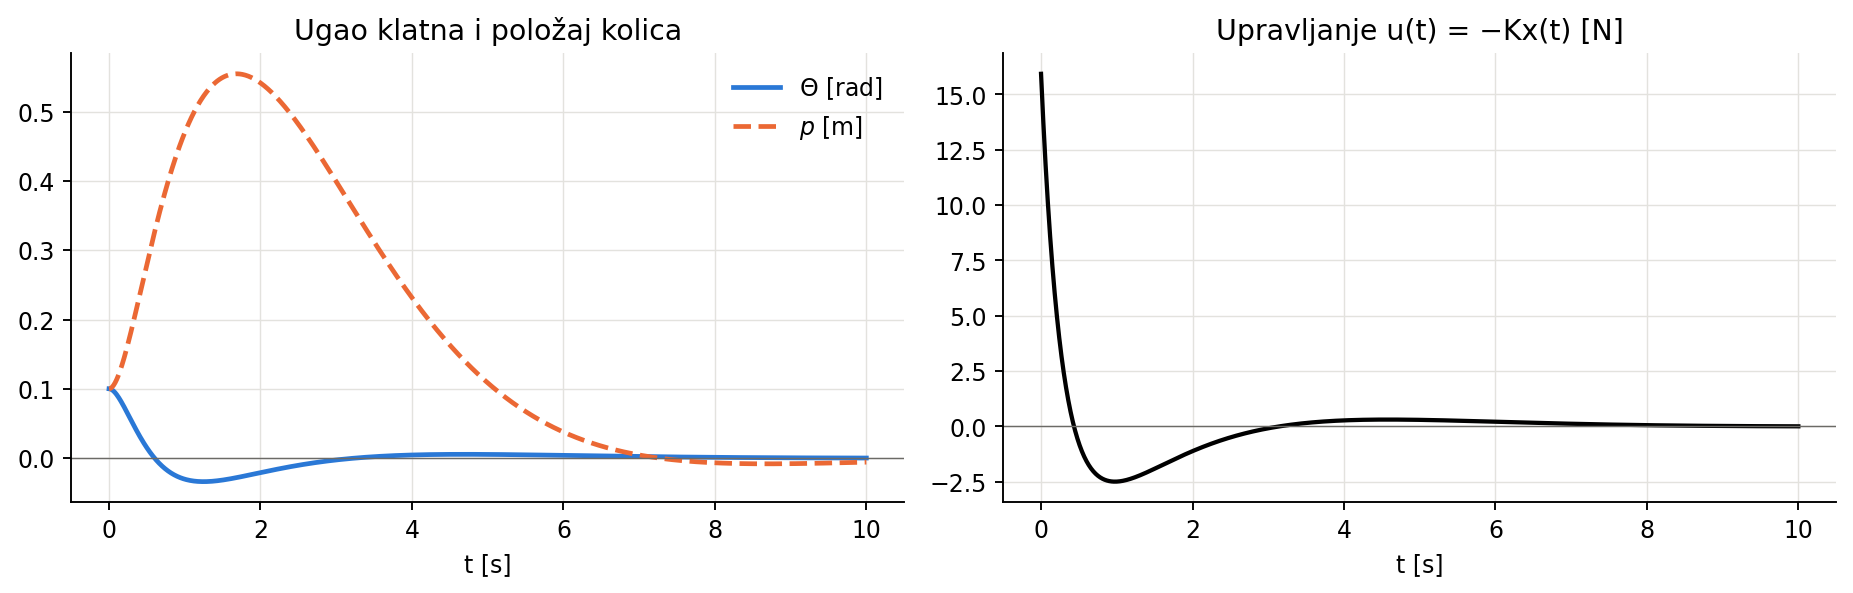
\includegraphics[width=0.95\linewidth,height=\textheight,keepaspectratio,alt={Primer 3. Levo: ugao klatna (puna linija) se vrati iz 0,1 rad u nulu za oko 2 s, uz mali podbačaj. Kolica (isprekidano) se prvo pomere do 0,55 m (moraju „podmetnuti'' oslonac pod klatno), pa se vrate u nulu za oko 7 s. Desno: sila počinje sa 16 N, kratko prelazi u negativno (do −2,5 N) i gasi se.}]{figures/q12_pr3.png}
\caption{Primer 3. Levo: ugao klatna (puna linija) se vrati iz 0,1 rad u nulu za oko 2 s, uz mali podbačaj. Kolica (isprekidano) se prvo pomere do 0,55 m (moraju „podmetnuti'' oslonac pod klatno), pa se vrate u nulu za oko 7 s. Desno: sila počinje sa 16 N, kratko prelazi u negativno (do −2,5 N) i gasi se.}
\end{figure}

\textbf{Šta reći.}

\begin{itemize}
\item Da bi se klatno koje pada udesno uspravilo, kolica moraju da krenu udesno, ispod njega. Zato je \(u(0) = 15{,}9\) N veliko i pozitivno, a kolica se prvo udalje od nule.
\item Posle toga je važno i vratiti kolica (težina 10 na \(p\)), što je sporije: dominantni par polova \(-0{,}60 \pm 0{,}45i\) određuje sporo vraćanje kolica.
\item Ugao ima 10 puta veću težinu od položaja, pa se prvo sređuje ugao.
\item Poređenje sa slajdom 30: maksimum položaja kolica oko 0,55 m u \(t \approx 1{,}7\) s, najveća negativna sila oko \(-2{,}5\) N u \(t \approx 1\) s. Poklapa se.
\end{itemize}

\begin{ispit}[{Pitanje 12}]
\begin{itemize}
\item Za svaki primer: postavka, Rikatijeva jednačina (ili \(K\)), šta se vidi na graficima.
\item Primer 1: uloga znaka \(a\) (stabilan ili nestabilan) i uloga \(\Psi\) (samo kraj intervala); \(P \to a\) za \(a > 0\), \(P \to 0\) za \(a < 0\).
\item Primer 2: \(P(t)\) se ustali, pa je \(K\) konstantno; uslovi: upravljivost, \(\Psi = 0\), konstantne matrice.
\item Primer 3: polovi pre i posle, fizičko objašnjenje kretanja kolica.
\item Domaći \izvor{P14 snimak, 69.--73. min}: primer 1 je teži, jer se simulira \textbf{vremenski promenljivo pojačanje} \(K(t)\) u povratnoj grani; primer 3 je „najlakši, 15 minuta'': \texttt{lqr}, sopstvene vrednosti \(A\) i \(A - BK\), pa ponoviti simulaciju za \textbf{različite \(Q\) i \(R\)} i prokomentarisati njihov uticaj na \(u\), \(\Theta\) i \(p\).
\item Zamka: \(I = \int\frac14u^2\) znači \(r = \frac12\) (zbog \(\frac12\) ispred integrala u opštoj formuli), pa je \(u = -2Px\).
\end{itemize}
\end{ispit}

\subsection{Moguća potpitanja}

\begin{itemize}
\item \textbf{Zašto je u primeru 1 za \(a = -0{,}2\) \(P \approx 0\)?} Nema člana \(qx^2\), a sistem se sam smiruje; upravljanje bi samo koštalo. Tek pred kraj, kad kazna \(\Psi\) postaje bitna, \(P\) raste ka \(\Psi\).
\item \textbf{Zašto je za \(a = 0{,}2\) \(P \approx 0{,}2\)?} Stacionarno rešenje za \(q = 0\) je \(P = \frac{r}{b^2}(a + |a|) = \frac12\cdot0{,}4 = 0{,}2\); tada je pol \(a - 2P = -0{,}2\), tj. nestabilan pol se preslika u simetričan stabilan.
\item \textbf{Zašto \(P(t)\) u primeru 2 pada na nulu pri kraju?} \(P(T) = \Psi = 0\): na samom kraju stanje više ništa ne košta, pa se regulator „opušta''. Daleko od kraja \(P\) je ustaljen.
\item \textbf{Da li je \(\Psi = 0\) uslov da se \(P\) ustali?} Profesor ga navodi kao jedan od tri Kalmanova uslova (upravljivost, Lagranžova forma, konstantne matrice) \izvor{P14 snimak, 61. min; slajd 27}, pa ga na ispitu treba navesti. Napomena: i u primeru 1 sa \(\Psi > 0\) \(P\) se ustali daleko od kraja, jer \(\Psi\) utiče samo na kraj intervala; za \(t_1 \to \infty\) taj uticaj nestaje.
\item \textbf{Kako se vežba uticaj \(Q\) i \(R\)?} Veće težine u \(Q\) daju brže smirivanje stanja i veće upravljanje; veće \(R\) štedi upravljanje, pa je odziv sporiji. U primeru 3 se to proverava ponavljanjem simulacije sa drugim \(Q\), \(R\) (domaći).
\item \textbf{Zašto se u primeru 3 koristi konstantno \(K\)?} Stabilizacija klatna traje neograničeno (\(t_1 \to \infty\)), pa je \(P\) rešenje algebarske Rikatijeve jednačine; pojačanje se ne menja u vremenu.
\item \textbf{Zašto kolica prvo idu od nule?} Klatno nagnuto udesno može da se uspravi samo ako se oslonac podmetne ispod njega; tek kad je ugao sređen, kolica se sporo vraćaju (dominantni polovi \(-0{,}60 \pm 0{,}45i\)).
\end{itemize}

\section{Dodatak: gradivo van liste pitanja}

Ovo nije na listi od 12 pitanja, ali je rađeno na predavanjima i može poslužiti kao dopunski primer uz pitanja 7 i 8 (ograničeno upravljanje). Kratko.

\subsection{Relejno upravljanje: nestabilan sistem sa jednim prekidanjem}

\[\dot x = 2x - u, \qquad x(0) = 2, \qquad \tfrac14 \le u \le 1, \qquad I = \int_0^1\Big(\frac x2 + u\Big)dt \to \min, \qquad x(1) \text{ slobodno.}\]

\textbf{Hamiltonijan.} \(H = \frac x2 + u + p(2x - u) = \big(\frac x2 + 2px\big) + (1 - p)\,u\). Koeficijent uz \(u\) je \(h = 1 - p\).

\textbf{Zašto ne \(\partial H/\partial u = 0\).} To bi dalo \(p \equiv 1\), a granični uslov je \(p(1) = 0\). Kontradikcija, pa je optimum na granici.

\textbf{Adjungovana promenljiva.} \(\dot p = -\frac12 - 2p\), \(p(1) = 0\). Partikularno rešenje je \(-\frac14\), homogeno \(Ce^{-2t}\):

\[p(t) = -\frac14 + \frac14e^{2(1 - t)} .\]

\(p\) je monotono opadajuće, pa je prekidanje najviše jedno. \(p(0) = \frac14(e^2 - 1) \approx 1{,}6 > 1\): na početku je \(h < 0\), pa \(u = u_{max} = 1\). Na kraju je \(p = 0 < 1\), pa \(u = u_{min} = \frac14\).

\textbf{Trenutak prekidanja} (\(p = 1\)): \(e^{2(1 - t_p)} = 5\), pa je \(t_p = 1 - \frac{\ln5}{2} = 0{,}195\). Stanje je neprekidno: na \([0, t_p]\) je \(x = \frac12 + \frac32e^{2t}\), pa je \(x(t_p) = 2{,}717\); na \([t_p, 1]\) je \(x = \frac18 + 1{,}754\,e^{2t}\).

\textbf{Poruka:} nestabilnom sistemu najveća pomoć treba na početku. Strategija je izabrana pomoću „tri pomoći'' iz odeljka „Zajednički alat'' (zdrav razum, \(p(1) = 0\), \(p(0)\)). Primer je rađen na predavanju dva puta \izvor{snimak 25.11, 0.--22. min; P11 snimak, 54.--72. min}; profesor kaže da „90\% literature'' relejno (bang-bang) upravljanje ilustruje baš ovakvim primerom.

\subsection{Roboti na Marsu (Majerov problem)}

Na Mars se pošalje \(x_0\) robota. Deo \(u \in [0, 1]\) robota pravi nove robote, a ostatak \(1 - u\) zida zgrade. Broj robota je \(x\), broj zgrada \(z\); cilj je \textbf{najviše zgrada u trenutku \(T\)} \izvor{snimak 25.11, 31.--61. min}:

\[\dot x = u\,x, \qquad \dot z = (1 - u)\,x, \qquad x(0) = x_0 > 0, \qquad z(0) = 0, \qquad z(T) \to \max .\]

Kriterijum sadrži samo krajnju vrednost (Majerov problem). Pošto je \(z(T) = \int_0^T(1 - u)x\,dt\), prevodi se u Lagranžov oblik.

\textbf{Hamiltonijan} (maksimizacija, pa je pravilo obrnuto): \(H = (1 - u)x + p\,u\,x = x + u\,x\,(p - 1)\). Pošto je \(x > 0\): \(u = 1\) za \(p > 1\), \(u = 0\) za \(p < 1\).

\textbf{Adjungovana jednačina.} \(\dot p = -\partial H/\partial x = -(1 - u) - p\,u\), a \(x(T)\) je slobodno, pa je \(p(T) = 0\). Znači da je na kraju \(p < 1\), tj. \(u = 0\): rešava se \textbf{unazad} od \(T\).

\begin{itemize}
\item Na \([t_p, T]\) (\(u = 0\)): \(\dot p = -1\), \(p = T - t\). Prekidanje je kad \(p = 1\): \(t_p = T - 1\).
\item Na \([0, t_p]\) (\(u = 1\)): \(\dot p = -p\), \(p = e^{t_p - t} > 1\). Strategija je dosledna.
\end{itemize}

\textbf{Rešenje.} Roboti se prvo samo množe (\(x = x_0e^t\)), a u poslednjoj jedinici vremena svi zidaju (\(x\) konstantno, \(z\) raste linearno): \(z(T) = x_0e^{T - 1}\) (za \(T > 1\); za \(T \le 1\) je \(u = 0\) ceo interval). Provera direktno: prekidanje u \(s\) daje \(z(T) = x_0e^s(T - s)\), a izvod \(e^s(T - s - 1) = 0\) daje \(s = T - 1\). Mešovito rešenje („40\% robota zida'') ovde ne postoji: \(p \equiv 1\) bi tražilo \(\dot p = -1 = 0\).

\subsection{Problem minimuma goriva}

Potrošnja goriva je srazmerna \textbf{apsolutnoj vrednosti} upravljanja (i kočenje troši gorivo), pa je kriterijum

\[J = \int_0^T|u|\,dt, \qquad |u| \le 1 .\]

(Kriterijum \(\int u^2dt\) je minimum \textbf{energije}: daje glatko upravljanje, kao u pitanju 6.)

\textbf{Tri vrednosti upravljanja.} Za \(H = b|u| + p\,f(x, u)\) sa \(f\) linearnim po \(u\) (član \(p\,u\)) razdvajaju se slučajevi \(u < 0\) (koeficijent \(-b + p\)) i \(u > 0\) (koeficijent \(b + p\)). Minimum \(H\):

\[u^* = \begin{cases} u_{min} = -1, & p > b \\ 0, & |p| < b \\ u_{max} = +1, & p < -b \end{cases}\]

To je \textbf{prošireno relejno upravljanje}, tj. tropoložajni regulator sa mrtvom zonom. Profesor: kad je upravljanje ograničeno, gotovo uvek se dobija relejno ili prošireno relejno (stepeničasto) upravljanje, a ovo drugo je karakteristično za potrošnju goriva; zato su prvi primeri teorije iz svemirskih letova \izvor{P11 snimak, 84.--87. min}. Vrednost 0 postoji jer se tako štedi gorivo (raketa u slobodnom padu).

\textbf{Primer}: \(\dot x = -x + u\), \(x(0) = 2\), \(x(2) = 0\), \(J = \int_0^2|u|\,dt\) (\(b = 1\)).

\begin{itemize}
\item \(\dot p = -\partial H/\partial x = p\), pa je \(p = Ce^t\): monotono, ali bez uslova na kraju (kraj je zadat), pa se strategija pretpostavlja.
\item Sistem je stabilan i sam ide ka nuli, pa se prvo pusti (\(u = 0\)), a na kraju se „dogura'' sa \(u = -1\). Vrednost \(u = +1\) nikad nije potrebna.
\item Na \([0, t_p]\): \(x = 2e^{-t}\); na \([t_p, 2]\): \(x = e^{2 - t} - 1\) (iz \(x(2) = 0\)). Neprekidnost: \(2e^{-t_p} = e^{2 - t_p} - 1\), pa je \(t_p = \ln(e^2 - 2) = 1{,}684\).
\item Provera: \(p(t_p) = b = 1\) daje \(p = e^{t - t_p}\); za \(t < t_p\) je \(0 < p < 1\) (\(u = 0\)), a za \(t > t_p\) je \(p > 1\) (\(u = -1\)). Potrošnja \(J = 2 - t_p = 0{,}316\).
\end{itemize}

\begin{figure}
\centering
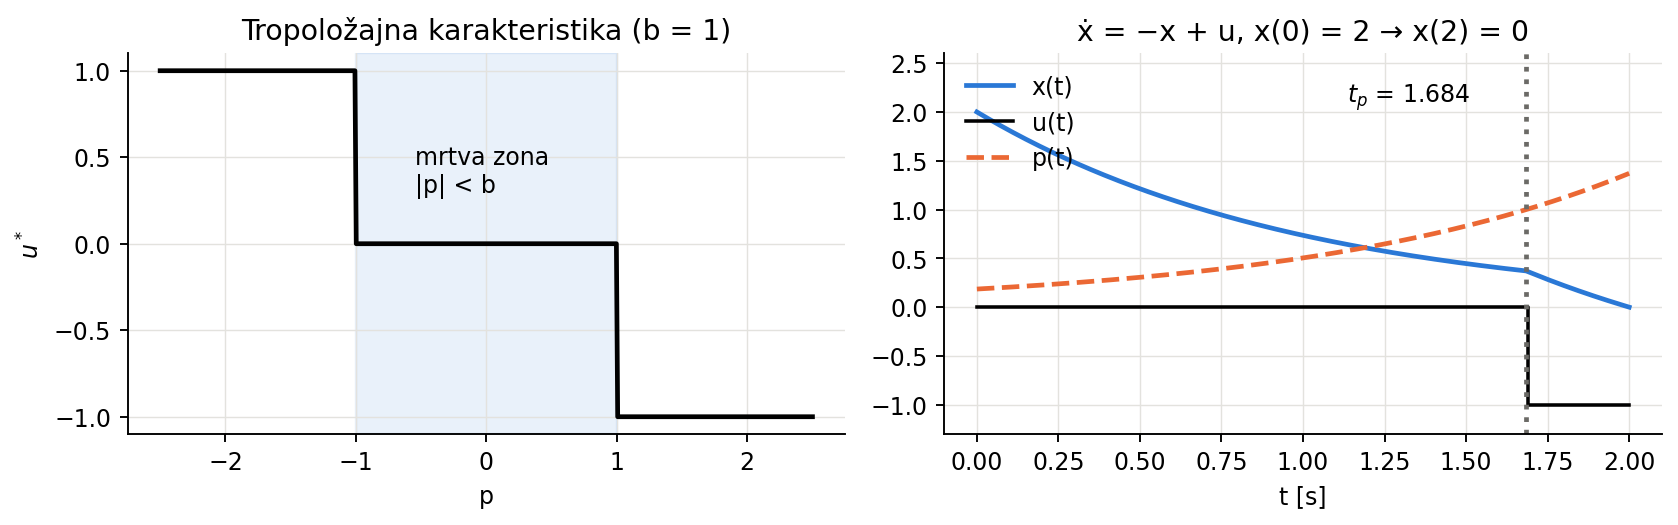
\includegraphics[width=0.9\linewidth,height=\textheight,keepaspectratio,alt={Minimum goriva. Levo: tropoložajna karakteristika u*(p) sa mrtvom zonom \textbar p\textbar{} \textless{} b. Desno: stabilan sistem se prvo pušta da sam opada (u = 0), a u tₚ = 1,684 uključuje se u = −1 tačno kad p(t) pređe prag b = 1, pa stanje stiže u nulu u t = 2.}]{figures/dod_gorivo.png}
\caption{Minimum goriva. Levo: tropoložajna karakteristika u*(p) sa mrtvom zonom \textbar p\textbar{} \textless{} b. Desno: stabilan sistem se prvo pušta da sam opada (u = 0), a u tₚ = 1,684 uključuje se u = −1 tačno kad p(t) pređe prag b = 1, pa stanje stiže u nulu u t = 2.}
\end{figure}

\begin{ispit}
Ako se na ispitu pomene relejno upravljanje ili minimum goriva, ključne rečenice su: \(H\) je linearan po \(u\) (ili po \(|u|\)), pa odlučuje znak koeficijenta uz \(u\); broj prekidanja zavisi od toga koliko puta taj koeficijent menja znak; strategija se pretpostavi rezonovanjem pa proveri preko \(p(t)\).

Profesor ovakve zadatke više ceni rešene \textbf{numerički} („probat ćete ih numerički, to mi je važnije'') \izvor{snimak 25.11-2, 38. min}.
\end{ispit}

\end{document}
